
\documentclass[11pt, reqno]{book}%{amsart}
\usepackage{graphicx}
\usepackage{xcolor}
\usepackage{amssymb}
\usepackage[margin=0.95in]{geometry}
\usepackage{fancyhdr}
\usepackage{amsmath}
\usepackage{caption}
\usepackage{array}
%\usepackage[T1]{fontenc}
\usepackage[utf8]{inputenc}
\usepackage{textcomp}
%\usepackage[scaled]{beramono}
\usepackage{tgcursor}
\usepackage[T1]{fontenc}
%\usepackage{tgbonum}
\usepackage[section]{placeins}
\setlength{\headheight}{15.2pt}
\pagestyle{fancy}

\fontfamily{cmr}

%\date{} 


\newcounter{ct}
\setcounter{ct}{0}
\newcommand{\aaproblem}{\addtocounter{ct}{1} \setcounter{aa}{0} \setcounter{equation}{0} \noindent \arabic{ct}.}
\newcounter{aa}
\setcounter{aa}{0}
\newcommand{\aapart}{\addtocounter{aa}{1} \noindent \textbf{\alph{aa}}) \smallskip}
\newcommand{\es}{\begin{equation}}
\newcommand{\ef}{\end{equation} \vspace{0.05in}}
\newcommand{\bes}{\begin{split}}
\newcommand{\fes}{\end{split}}
\newcommand{\mbf}{\mathbf}
\newcommand{\mbfg}[1]{\mbf{\mbox{\boldmath$#1$}}}
\newcommand{\mbfgh}[1]{\hat{\mbfg{#1}}}
\newcommand{\mbfh}[1]{\hat{\mbf{#1}}}
\newcommand{\ua}{\uparrow}
\newcommand{\da}{\downarrow}
\newcommand{\p}{{^\prime}}
\newcommand{\citep}{} % so I don't have to constantly change things between the standalones and the real tex files
\newcommand{\nstf}{\textcolor{blue}}
%\newcommand{\nstf}{}
\newcommand{\ola}{\overleftarrow}
\newcommand{\ora}{\overrightarrow}
\newcommand{\ve}{\varepsilon}
\newcommand{\tens}{\overset{\text{\tiny$\leftrightarrow$}}}
\newcommand{\tw}[1]{{\tt #1}}
\newcommand{\clr}{\color{blue}}
\newcommand{\clb}{\color{black}}
%\newcommand{\vtm}[1]{\begin{verbatim}{#1}\end{verbatim}}



%\setkomafont{author}{\scshape}
%\usepackage{blindtext}
\title{WaveCalc}
%\subtitle{The Wave Calculator}
\author{Ryan Goetz \thanks{rgoetz@phys.ufl.edu}}
%\subtitle{A closer look at the expenses}
%\subject{a funny paper}


\begin{document}

%\title{The Wave Calculator}
%\author{Ryan Goetz}
%\date{\today}
\maketitle

\lhead[Ryan Goetz]{WaveCalc}
\rhead[\today]{\today}


\tableofcontents




%%%%%%%%%%%%%%%%%%%%%%%%%%%%%%%%%%%%%%%%%%%%%%%%%%%%%%%%%%%%%%%%%%%%%%
%%%%%%%%%%%%%%%%%%%%%%%%%%%%%%%%%%%%%%%%%%%%%%%%%%%%%%%%%%%%%%%%%%%%%%
%%%%%%%%%%%%%%%%%%%%%%%%%%%%%%%%%%%%%%%%%%%%%%%%%%%%%%%%%%%%%%%%%%%%%%
%%%%%%%%%%%%%%%%%%%%%%%%%%%%%%%%%%%%%%%%%%%%%%%%%%%%%%%%%%%%%%%%%%%%%%
%%%%%%%%%%%%%%%%%%%%%%%%%%%%%%%%%%%%%%%%%%%%%%%%%%%%%%%%%%%%%%%%%%%%%%
\chapter{The Wave Calculator}
\label{chap:intro}

\section{Motivating a Wave Tool}
\label{sec:motivation}

Much of the utility, depth, and breadth of experimental optics is predicated upon the wealth of electromagnetic wave interactions with optical materials. From materials we build lenses, mirrors, prisms, polarizers, retarders, rotators, isolators, gratings, modulators, resonators, and all sorts of things between. Even in optical experiments wherein the signal of interest is generated by a laser field's propagation through vacuum, there will undoubtedly be a plethora of these aforementioned optical components whose role is to condition the field for its scientific purpose.

Unfortunately, if the reader has only been exposed to optical phenomena as taught in the standard electromagnetism courses, they are likely only familiar with a small subset of wave behavior in materials. Particularly, common core coursework will often restrict itself to isotropic media, only very rarely stepping out into the muddier waters of anisotropy, and even then only considering highly sanitized cases. As an example, most students and optics researchers will be well-versed in the basic operating principle behind a half-wave plate. Two orthogonal polarizations in the medium undergo a differential phase shift of $\pi$ over the length of the material, and so the effect on any incoming field whose linear polarization is not entirely in one of these special directions is that the polarization has been rotated upon exit. But what happens when the waveplate moves from the paper to the laboratory, where it must be fixed in a physical mount and aligned to a laser field (likely by hand)? How does the output field change as the waveplate is pitched and yawed about the beam axis? Most people in the field of optics will understand that such misalignments give rise to ellipticity of the output field, but how much? How do we quantify the coupling between ellipticity and misalignment? And are there more effects to which we are unaware? Technically, anyone who has exposure to Maxwell's equations has the framework to answer these questions, however the path to the answers is not so short and for many has never been tread. In large part, this lack of exposure to the fuller picture of electromagnetism motivated the creation of the WaveCalc tool.

In isotropic media, electromagnetic wave behavior is both well-understood and straightforward to calculate. The propagation of waves within the medium is nearly identical to the case of wave solutions in free space. Electric fields oscillate in the plane of their phase-fronts. Rules governing reflection and transmission of waves across media boundaries can be written in greatly simplified forms, far removed from the vector and tensor calculus of Maxwell's equations. What results are familiar relationships such as Snell's Law, the Law of Reflection, or the Fresnel equations. However, when we extend the analysis beyond isotropic media, we quickly discover that these well-known and reliable rules are merely special cases of more complicated--yet more fundamental--results.

In designing WaveCalc, we sought to construct a tool capable of examining electromagnetic wave behavior in the simplest case: plane waves in linear, non-permeable, dielectric media. Though not physically realizable, plane waves are reasonable models of laser fields for many applications. Similarly, many optical media of interest can be approximated as linear dielectrics; material in which there is no free charge and the electric displacement responds linearly to an incident electric field. Even in nonlinear media, the nonlinear terms are often small enough that the contribution from the laser's own electric field is negligible. We do not extend out analysis beyond dielectrics, as media in which there are free charges tend to quickly attenuate electromagnetic waves, and therefore are usually less interesting as optical materials.

Chapter \ref{chap:theory} discusses the theoretical background for calculating plane wave behavior in linear dielectric materials; beginning from Maxwell's equations to enumerate the plane-wave modes of a medium, and ultimately characterizing the interaction of a wave with a media boundary. Chapter \ref{chap:implement} then addresses how the results of Chapter \ref{chap:theory} might be implemented algorithmically to incorporate into a calculation tool. Chapters \ref{chap:wavecalcobj} and beyond introduce the \tw{wavecalc} Python package, and explain how it can be used to perform calculations of interest.




\section{\tw{wavecalc}}
\label{sec:wavecalcpack}


The implementations outlined in Chapter \ref{chap:implement} have been coded in Python and packaged as \tw{wavecalc}. This package provides tools for easily calculating plane wave behavior in dielectric media and at the interface of media. Both as attributes, function arguments, and core functions, WaveCalc relies heavily on objects from the \tw{numpy} package; and so this package is a dependency for \tw{wavecalc}.

In this text we will use example code to illustrate the properties and functionality of the \tw{wavecalc} package. In doing so, we use the convention that any line beginning with \verb|>>| is input code, and any line following is an output of the input code:
\begin{verbatim}
>> input code
output of code
\end{verbatim}
With the exception of the line above, all example code in this text should be executable by the reader if done in the order presented. Lines that are neither input code nor following input code are often intended to give an understanding of syntax, but are not intended to be passed to an interpreter.

Technically, in Python everything is an object, however it makes sense to distinguish between the Python objects which are representative of physical entities and the Python objects which are representative of physical processes. The former we refer to as objects, and the latter as functions. Chapter \ref{chap:wavecalcobj} introduces these WaveCalc objects, Chapter \ref{chap:methods} explains the methods associated with these objects, and Chapter \ref{chap:wavecalcfun} describes the primary set of WaveCalc functions. In Chapter \ref{chap:examp}, we will demonstrate the utility of WaveCalc with some examples. Chapter \ref{chap:algebra} is included as an interesting investigation into the algebra of some WaveCalc operations, but is not necessary to understand the usage of \tw{wavecalc}.

To work with WaveCalc and follow along with the example code, the user will need to import the \tw{wavecalc} package into their Python interpreter. And because a great number of WaveCalc objects have \tw{numpy} objects as attributes, it is recommended to also import \tw{numpy} whenever planning to use \tw{wavecalc}:
\begin{verbatim}
>> import wavecalc as wc
>> import numpy
Importing wavecalc.classes as obj
Importing wavecalc.functions as fun
\end{verbatim}
\noindent The reader will notice that we have chosen to alias \tw{wavecalc} as \tw{wc}. We do so in the interest of brevity, and hopefully not at the expense of clarity for the reader. 















.








%%%%%%%%%%%%%%%%%%%%%%%%%%%%%%%%%%%%%%%%%%%%%%%%%%%%%%%%%%%%%%%%%%%%%%
%%%%%%%%%%%%%%%%%%%%%%%%%%%%%%%%%%%%%%%%%%%%%%%%%%%%%%%%%%%%%%%%%%%%%%
%%%%%%%%%%%%%%%%%%%%%%%%%%%%%%%%%%%%%%%%%%%%%%%%%%%%%%%%%%%%%%%%%%%%%%
%%%%%%%%%%%%%%%%%%%%%%%%%%%%%%%%%%%%%%%%%%%%%%%%%%%%%%%%%%%%%%%%%%%%%%
%%%%%%%%%%%%%%%%%%%%%%%%%%%%%%%%%%%%%%%%%%%%%%%%%%%%%%%%%%%%%%%%%%%%%%
\chapter{Plane Waves in Dielectric Materials}
\label{chap:theory}

In this chapter we lay the groundwork for the physical theory behind the machinations of WaveCalc. In Section \ref{sec:bookerquart} we will enumerate the plane-wave modes permitted in a dielectric medium. In Section \ref{sec:opticaxis} we will examine these modes to identify special directions in the medium, referred to as optic axes. In Section \ref{sec:kboundary} we will show how boundary conditions can be applied to relate the wave vector on either side of a material boundary. Section \ref{sec:Eboundary} addresses boundary conditions on the electric field, and how they may be used to compute reflected and transmitted fields. 




%%%%%%%%%%%%%%%%%%%%%%%%%%%%%%%%%%%%%%%%%%%%%%%%%%%%%%%%%%%%%%%%%%%%%%
\section{Wave Propagation in a Medium and the Booker Quartic}
\label{sec:bookerquart}

Maxwell's equations in a dielectric material (no free charges or currents) read:
\es
\begin{array}{ccc}
\nabla\cdot \mbf{D}= 0 & & \nabla\cdot \mbf{B}=0 \\
& & \\
\nabla \times \mbf{E} = -\frac{\partial \mbf{B}}{\partial t} & & \nabla\times \mbf{H} = \frac{\partial \mbf{D}}{\partial t}
\end{array}
\ef
\noindent For a linear medium the displacement vector is related to the electric field by the permittivity tensor:
\es
 \mbf{D} = \ve_0 \tens{\mbfg{\ve}}\cdot \mbf{E}
 \label{eq:displacevec}
 \ef
 \noindent here we have chosen the convention such that $\tens{\mbfg{\ve}}$ is unitless. In the simple case which we consider, $\tens{\mbfg{\ve}}$ is both spatially and temporally independent. Further, we suppose that the medium is non-permeable, that is $\mu_0 \mbf{H} = \mbf{B}$. Under these assumptions, we can eliminate the magnetic fields and write:
 \es
 \nabla\times\nabla\times \mbf{E} = -\mu_0 \frac{\partial^2 \mbf{D}}{\partial t^2}
 \label{eq:doublecrossE}
 \ef
 \noindent As we are interested in wave solutions to Maxwell's equations, our ansatz is a plane-wave electric field:
\es
\mbf{E} = \mbf{E}_0 e^{i(\mbf{k}\cdot \mbf{r}-\omega t)}
\label{eq:ansatz}
\ef
\noindent where $\mbf{E}_0$ is a spatially and temporally invariant vector which encodes the amplitude and polarization of the wave, $\mbf{k}$ is called the wave vector and determines how the phase of the wave evolves through space, and $\omega$ is a scalar which determines how the phase evolves over time. We have made the common conventional choice to represent the electric field with a complex-valued vector. This helps to simplify the algebra and calculus, however the reader should keep in mind that the physically meaningful quantity is the real part of this complex vector.

Using (\ref{eq:displacevec}) and (\ref{eq:ansatz}) along with the identity $\nabla\times\nabla\times \mbf{E} = \nabla(\nabla\cdot\mbf{E})-\nabla^2\mbf{E}$, we can rewrite (\ref{eq:doublecrossE}) as an algebraic equation:
\es
 -(\mbf{k}\cdot \mbf{E}) \mbf{k} +k^2 \mbf{E}= \mu_0\ve_0 \omega^2 \tens{\mbfg{\varepsilon}}\cdot \mbf{E}
 \label{eq:maxwelleqjustE}
\ef
\noindent where $k^2 = \mbf{k}\cdot \mbf{k}$. We have arrived at what the author considers to be the most disappointing of all electromagnetic equations. Invariably, (\ref{eq:maxwelleqjustE}) shows up in textbooks throughout all time and space, though in its present form its utility is limited; and for our cause it will be limited to providing a solitary insight. In the event that the medium is vacuum, $\tens{\mbfg{\ve}}$ becomes the identity, and the Maxwell equation $\nabla\cdot \mbf{D} =0$ causes the first term on the left-hand side of (\ref{eq:maxwelleqjustE}) to vanish. When this happens, we see that the wave number of vacuum, denoted $k_0$, can be related to the angular frequency of the wave, $\omega$, and fundamental constants by $k^2_0 = \mu_0 \ve_0 \omega^2$. Evidently, all electromagnetic waves in vacuum propagate with speed $c = 1/\sqrt{\mu_0\ve_0}$, the so-called speed of light.

As far as we are concerned, the usefulness of the form of (\ref{eq:maxwelleqjustE}) has been exhausted. In its stead, we reconstruct (\ref{eq:maxwelleqjustE}) as an eigenvector equation:
\es
\left(\mbf{k}\otimes \mbf{k}+k^2_0 \tens{\mbfg{\ve}}\right)\cdot \mbf{E} = k^2 \mbf{E}
\label{eq:eigenequationmaxwell}
\ef
\noindent where the $\mbf{k}\otimes\mbf{k}$ denotes the outer product of the wave vector with itself. We see that wave solutions for the electric field are eigenvectors of the operator $\mbf{k}\otimes\mbf{k} +k^2_0 \tens{\mbfg{\ve}}$ with eigenvalues $k^2$. We pause here for a moment, as this result is fundamental: every plane wave mode of a medium having the form given in (\ref{eq:ansatz}) has a field amplitude vector which is an eigenvector of the operator on the left-hand side of (\ref{eq:eigenequationmaxwell}). We will call this operator the Maxwell wave operator. Further, every plane wave mode must have a wave vector whose self dot product is an eigenvalue of the electric field amplitude vector under the Maxwell wave operator. 

The eigenvalues of the Maxwell wave operator are the roots of the characteristic equation: 
\es
\left| \mbf{k}\otimes \mbf{k}+k^2_0 \tens{\mbfg{\ve}} -k^2\tens{\mbf{I}} \right| =0
\label{eq:charequation}
\ef
\noindent which constitutes a condition on the wave vector $\mbf{k}$. Though when writing out the terms it might initially appear to be a sixth-order equation in $k$, the highest order terms cancel and we are left with a quartic that can be written in Cartesian coordinates as:
\es
\begin{split}
0 =&k^4_0 \left| \tens{\mbfg{\varepsilon}} \right|-k^2_0\left[k^2_x\left(M_{yy}+M_{zz}\right) +k^2_y \left(M_{xx}+M_{zz} \right) +k^2_z \left( M_{xx}+M_{yy}\right)  \right] \\
& -k^2_0 \left[k_x k_y \left(M_{xy}+M_{yx}\right) +k_y k_z \left( M_{yz}+M_{zy}\right) -k_x k_z \left(M_{xz}+M_{zx}\right)  \right] \\
& +  k^2 \left[k^2_x \varepsilon_{xx} +k^2_y \varepsilon_{yy} +k^2_z \varepsilon_{zz}+k_xk_y \left(\ve_{xy}+\ve_{yx}\right)+k_y k_z\left(\ve_{yz}+\ve_{zy}\right) +k_x k_z \left(\ve_{xz}+\ve_{zx} \right)\right]
\end{split}
\ef
\noindent where $M_{ij}$ are the minors of the permittivity tensor. By some true genius or dumb luck (I don't have access to most of the publications discussing it), somebody discovered that this could be expressed in the more compact form:
\es
0 = k^2 \left(\mbf{k}\cdot\tens{\mbfg{\ve}}\cdot\mbf{k} \right) +k^2_0  \mbf{k}\cdot \left\{\mbox{adj}\left(\tens{\mbfg{\ve}}\right)-\mbox{tr}\left[\mbox{adj}\left(\tens{\mbfg{\ve}}\right) \right] \tens{\mbf{I}}  \right\} \cdot \mbf{k} +k^4_0 \left| \tens{\mbfg{\ve}} \right|
\label{eq:bookerquartic}
\ef
\noindent When written in this form, (\ref{eq:bookerquartic}) is known as the Booker quartic. I really wish I could derive this from (\ref{eq:charequation}) without brute force; it's so pretty. Though the general solution to quartic equations can be quite involved, notice that (\ref{eq:bookerquartic}) is biquadratic (it only involves even powers of $k$), and so if we define:
\es
\begin{array}{l}
A= \mbfh{k}\cdot\tens{\mbfg{\ve}}\cdot\mbfh{k}\\
B = k^2_0  \mbfh{k}\cdot \left\{\mbox{adj}\left(\tens{\mbfg{\ve}}\right)-\mbox{tr}\left[\mbox{adj}\left(\tens{\mbfg{\ve}}\right) \right] \tens{\mbf{I}}  \right\} \cdot \mbfh{k} \\
C= k^4_0 \left| \tens{\mbfg{\ve}} \right|
\end{array}
\label{eq:bookercoeffs}
\ef
\noindent then the solutions of the companion equation:
\es
0 = q^2 \left(\mbfh{k}\cdot\tens{\mbfg{\ve}}\cdot\mbfh{k} \right) +q k^2_0  \mbfh{k}\cdot \left\{\mbox{adj}\left(\tens{\mbfg{\ve}}\right)-\mbox{tr}\left[\mbox{adj}\left(\tens{\mbfg{\ve}}\right) \right] \tens{\mbf{I}}  \right\} \cdot \mbfh{k} +k^4_0 \left| \tens{\mbfg{\ve}} \right|
\label{eq:companionquadratic}
\ef
\noindent given by:
\es
q_{\pm} = \frac{-B \pm \sqrt{B^2-4A C}}{2A}
\label{eq:companionsolutions}
\ef
\noindent lead directly to the solutions of (\ref{eq:bookerquartic}):
\es
\begin{array}{lcr}
k_{a+} =\sqrt{q_-} & \quad& k_{a-}= -\sqrt{q_-} \\
&\quad &  \\
k_{b+} = \sqrt{q_+} & \quad& k_{b-} = - \sqrt{q_+}
\end{array}
\label{eq:bookersolutions}
\ef
\noindent We should be careful not to confuse the solutions given by (\ref{eq:bookersolutions}) with the magnitude of $\mbf{k}$ (as well should be obvious since magnitudes are never negative). Instead, for any given unit vector $\mbfh{k}$, the solutions to the Booker quartic yield the allowed wave vectors by $k_{(a,b)(+,-)}\mbfh{k}$. We therefore interpret the left and right columns of (\ref{eq:bookersolutions}) as the forward and backward propagating waves, respectively. For this reason, we might sometimes choose to drop the second subscript and simply write $k_a$ and $k_b$ as the wave solutions. The biquadratic nature of the Booker quartic for a fixed $\mbfh{k}$ reflects the symmetry of forward and backward propagation.

As a direct consequence of Maxwell's equations for linear dielectrics, we have found that for any given propagation direction and frequency there are two wave vectors allowed by the medium. We refer to these two waves as the $a$-wave and the $b$-wave. Each of these waves have electric fields which are eigenvectors of the corresponding operator $\mbf{k}\otimes\mbf{k} +k^2_0 \tens{\mbfg{\ve}}$. %When the discriminant in (\ref{eq:companionsolutions}) vanishes, the $a$- and $b$-waves are degenerate in their wave vectors; we call this special direction an optic axis of the medium.




%%%%%%%%%%%%%%%%%%%%%%%%%%%%%%%%%%%%%%%%%%%%%%%%%%%%%%%%%%%%%%%%%%%%%%

\section{Optic Axes of a Dielectric Medium}
\label{sec:opticaxis}



When the discriminant in (\ref{eq:companionsolutions}) vanishes, the $a$- and $b$-waves are degenerate in their wave vectors, and therefore also their field eigenvectors. We call this special direction an optic axis of the medium. Waves traveling along the optic axis will propagate as though the medium were isotropic. This condition as explicitly written:
\es
B^2-4AC = 0
\label{eq:opticaxiscond}
\ef
\noindent is in general a condition on both $\mbfh{k}$ and $\tens{\mbfg{\ve}}$.




%%%%%%%%%%%%%%%%%%%%%%%%%%%%%%%%%%%%%%%%%%%%%%%%%%%%%%%%%%%%%%%%%%%%%%
\clr
\subsection{Isotropic Media: UNDER CONSTRUCTION}
\label{sec:isomedia}

By definition, in an isotropic medium the permittivity tensor must remain invariant for any choice of orthonormal basis, and therefore is a scalar multiple of the identity: $\tens{\mbfg{\ve}}=\ve\tens{\mbf{I}}$. In this case, the quartic coefficients simplify greatly:
\es
\begin{array}{l}
A = \ve \mbfh{k} \cdot \tens{\mbf{I}}\cdot \mbfh{k} = \ve \\
B=k^2_0 \mbfh{k}\cdot\left(\ve^2\tens{\mbf{I}}-3\ve^2\tens{\mbf{I}}\right)\cdot\mbfh{k} = -2\ve^2 k^2_0 \\
C=  \ve^3 k^4_0
\end{array}
\ef
\noindent from which we can see that equality in (\ref{eq:opticaxiscond}) is always satisfied. The allowed wave vectors are easily found:
\es
k_\pm = \pm \sqrt{\ve}k_0 
\ef


\clb

%%%%%%%%%%%%%%%%%%%%%%%%%%%%%%%%%%%%%%%%%%%%%%%%%%%%%%%%%%%%%%%%%%%%%%
\clr
\subsection{Uniaxial Media: UNDER CONSTRUCTION}
\label{sec:unimedia}

\es
\tens{\mbfg{\ve}}=
\left(\begin{array}{ccc}
\ve_1 & 0 & 0 \\
0 & \ve_1 & 0 \\
0 & 0 &\ve_2
\end{array}\right)
\ef

\es
\begin{array}{l}
A = \ve_1 \hat{k}^2_x +\ve_1 \hat{k}^2_y +\ve_2 \hat{k}^2_z
\end{array}
\ef







\clb
%%%%%%%%%%%%%%%%%%%%%%%%%%%%%%%%%%%%%%%%%%%%%%%%%%%%%%%%%%%%%%%%%%%%%%
\clr
\subsection{Biaxial Media: UNDER CONSTRUCTION}
\label{sec:bimedia}


\es
\tens{\mbfg{\ve}}=
\left(\begin{array}{ccc}
\ve_x & 0 & 0 \\
0 & \ve_y & 0 \\
0 & 0 &\ve_z
\end{array}\right)
\ef

\es
\begin{array}{l}
A = \ve_x \hat{k}^2_x +\ve_y \hat{k}^2_y +\ve_z \hat{k}^2_z \\
B = -k^2_0 \left[ \ve_x\left(\ve_y+\ve_z\right)\hat{k}^2_x + \ve_y\left(\ve_x+\ve_z\right)\hat{k}^2_y +\ve_z\left(\ve_x+\ve_y\right)\hat{k}^2_z  \right] \\
C= k^4_0\ve_x \ve_y \ve_z
\end{array}
\ef

\es
0= \left[\ve_x\left(\ve_y+\ve_z\right)\hat{k}^2_x + \ve_y\left(\ve_x+\ve_z\right)\hat{k}^2_y +\ve_z\left(\ve_x+\ve_y\right)\hat{k}^2_z  \right]^2 - 4 \ve_x\ve_y \ve_z \left( \ve_x \hat{k}^2_x +\ve_y \hat{k}^2_y +\ve_z \hat{k}^2_z \right)
\ef



\clb

%%%%%%%%%%%%%%%%%%%%%%%%%%%%%%%%%%%%%%%%%%%%%%%%%%%%%%%%%%%%%%%%%%%%%%
\section{Wave Vector Boundary Conditions}
\label{sec:kboundary}

As much of our interest is in characterizing wave behavior at media interfaces, we are not content to enumerate the optical modes in a dielectric: we must also understand how a wave incident on a medium reflects and transmits. When considering a boundary, whatever the material properties on either side, it must be the case that the phase of the wave is continuous at the boundary. More explicitly, the phase of the incoming wave must equal the phase of the refracted wave which must equal the phase of the reflected wave (or be 180 degrees out of phase depending on your perspective). In terms of the wave vectors of the three waves, this must mean that their components tangent to the surface normal must all be equal. Specifically, if $\mbfh{s}$ is the normal vector to the boundary, and $\mbf{k}_i$, $\mbf{k}_j$ are wave vectors corresponding to the incoming or outgoing waves, then:
\es
\mbfh{s}\times(\mbf{k}_i-\mbf{k}_j) =0
\ef
\noindent This observation enables a convenient choice for coordinate system. Let the boundary be the $x$-$y$ plane, with the incoming media, $\tens{\mbfg{\ve}}_1$, corresponding to $z<0$ and the outgoing media, $\tens{\mbfg{\ve}}_2$, to $z>0$. If the tangential component of the incoming (or reflected or refracted) wave vector is non-zero, choose the $x$-axis so that $\mbf{k}_\perp = \rho \mbfh{x}$ for some constant $\rho$. In the event that the tangential component is zero, the choice of $x$- and $y$- axes can be made at the reader's convenience.  


%, then $k_x$ and $k_y$ of the outgoing wave are fixed to be the same as that for the incoming wave. 

%Might want to choose $x$-axis so that $\mbf{k}_\perp = \rho \mbfh{x}$ for some constant $\rho$.

With this convention, we know that all waves under consideration must have equal $k_x$ and $k_y=0$. For brevity, it is helpful to define the following two tensors for the media on either side of the boundary: $\tens{\mbfg{\sigma}}= \tens{\mbfg{\ve}}+(\tens{\mbfg{\ve}})^T$ and $\tens{\mbfg{\delta}}= \mbox{tr}(\tens{\mbfg{\ve}})\tens{\mbf{I}}-\tens{\mbfg{\ve}}$. Then, adopting notation from Pettis (mostly), we let:


\es
\begin{array}{l}
\Delta_j = k_x\sigma^{(j)}_{xz}\\
\\
\Sigma_j =k^2_x\delta^{(j)}_{yy}-k^2_0 \left(M^{(j)}_{xx}+M^{(j)}_{yy}\right) \\
\\
\Psi_j = k^3_x\sigma^{(j)}_{xz}+k^2_0 k_x\left(M^{(j)}_{xz}+M^{(j)}_{zx}\right)\\
\\
\begin{split}
\Gamma_j &= k^4_x \ve_{xx}-k^2_0 k^2_x\left(M^{(j)}_{yy}+M^{(j)}_{zz}\right) +k^4_0 \left|\tens{\mbfg{\ve}}_j  \right|
\end{split}
\end{array}
\label{eq:bookercoeffsnewcoords}
\ef
\noindent Here $j$ is the index of the medium; for the reflected case $j=1$, and for the transmitted case $j=2$. We can rewrite the Booker quartic from (\ref{eq:bookerquartic}) as an equation in $k_z$:
\es
\ve_{zz} k^4_z +\Delta_j k^3_z+\Sigma_j k^2_z +\Psi_j k_z +\Gamma_j =0
\label{eq:kvecequation}
\ef
\noindent Unlike in the previous subsection, this quartic is not identically biquadratic, nor in general would we expect it to be: we have not fixed a propagation direction, but instead fixed the tangential component of the wave vector. In the event that $k_x=0$, we can see from (\ref{eq:bookercoeffsnewcoords}) that the odd-order terms vanish and we recover the biquadratic; because in this special case we are fixing $\mbf{k}$ to be in the $z$-direction.

What we gather from (\ref{eq:kvecequation}) is that an incoming mode to a boundary has four corresponding modes in both the incident and transmission media. What may be less immediately obvious is that the incoming mode will excite two modes in the incident media, corresponding to waves with $k_z<0$, and two modes in the transmission media with $k_z>0$. Thus, a wave incident on a material boundary gives rise to four new waves. This is a departure from the more familiar case of isotropic media, where every incoming wave has one reflected and one transmitted wave. As it happens, when the materials are isotropic, the two reflected waves share a wave vector, and the same for the transmitted waves, and hence can be considered one wave each.

At this point it is worthwhile to pause and reflect on our results to this point; there is a subtlety which would be easy to miss but has important implications for our tool. In Section \ref{sec:bookerquart} we derived the Booker quartic from Maxwell's equations and a plane-wave solution ansatz, given as (\ref{eq:bookerquartic}). This equation defines a surface, $\mathcal{S}$, of the allowed wave vector modes of a medium, and this surface has the following property: for any unit vector $\mbfh{u}$, there are two associated scalars, $\kappa_a$, $\kappa_b$, such that $\pm \kappa_a \mbfh{u}$ and $\pm \kappa_b \mbfh{u}$ lie on the surface. Because the unit sphere is compact in $\mathbb{C}^3$, and the roots of the Booker quartic are continuous for continuously varying vector directions, the surface over complex 3-space is bounded. Because of this, every component of any vector $\mbf{k}\in\mathcal{S}$ is also bounded. However our analysis above places no such restraint on the $k_x$ component, for example. Indeed, for any value of $k_x$, (\ref{eq:kvecequation}) will yield solutions for $k_z$. How is this not a contradiction? 


% 1) for any vector $\mbf{u}$, there are four associated scalars $\kappa_i$, $i = 1,2,3,4$, such that $\kappa_i \mbf{u}$ is on the surface, and 2) if a vector $\mbf{w}$ lies on the surface, so does $-\mbf{w}$.


%interactions spanning two media, with permittivity tensors $\tens{\mbfg{\ve}}_1$ and $\tens{\mbfg{\ve}}_2$ respectively



%%%%%%%%%%%%%%%%%%%%%%%%%%%%%%%%%%%%%%%%%%%%%%%%%%%%%%%%%%%%%%%%%%%%%%

\section{Electric Field Boundary Conditions}
\label{sec:Eboundary}

In the previous section we outlined how a resultant wave vector can be related to an input wave. However, this is only half of the story: to fully describe the resultant wave we need the fields as well. Without information on how the fields are reflected and transmitted at an interface, we would be incapable of exploring many common phenomenon of optically interesting dielectrics such as: double refraction, optical activity, polarization, and more.

Suppose we have two media, labeled medium 1 and medium 2, connected by a planar boundary with unit surface normal $\mbfh{s}$. As we saw in Section \ref{sec:kboundary}, every wave incident on a boundary will result in four new waves: two reflected waves, and two transmitted waves. Thus, the electric field on one side of the boundary is the sum of three waves, the incident and two reflected, while the field on the other side is the sum of the two transmitted waves. In general, we will only be given the incident wave, and must calculate the four other waves.

Label the reflected waves $\alpha$ and $\beta$, with wave vectors $\mbf{k}_\alpha$ and $\mbf{k}_\beta$, and label the transmitted waves $\gamma$ and $\nu$ with wave vectors $\mbf{k}_\gamma$ and $\mbf{k}_\nu$. Name the corresponding reflected and transmitted electric field amplitude vectors $\mbfg{\alpha}$, $\mbfg{\beta}$, $\mbfg{\gamma}$, and $\mbfg{\nu}$. In this way, we can write the fields on either side of the boundary (without time dependence) as:
\begin{subequations}
\begin{align}
\mbf{E}_1 &= \mbf{E}_{i} e^{i \mbf{k}_i \cdot \mbf{r}} + \mbfg{\alpha}e^{i\mbf{k}_\alpha \cdot \mbf{r}} +\mbfg{\beta} e^{i\mbf{k}_\beta \cdot \mbf{r}} \\
\mbf{E}_2 & = \mbfg{\gamma}  e^{i\mbf{k}_\gamma\cdot \mbf{r}} + \mbfg{\nu} e^{i\mbf{k}_\nu \cdot \mbf{r}}
\end{align}
\label{eq:fieldseitherside}%
\end{subequations}
\noindent here of course, $\mbf{E}_i e^{i\mbf{k}_i \cdot \mbf{r}}$ is the incident wave. From Section \ref{sec:bookerquart}, we know the reflected and transmitted fields must be eigenvectors of their respective Maxwell wave operators:
\begin{subequations}
\begin{align}
\left(\mbf{k}_\alpha \otimes \mbf{k}_\alpha +k^2_0 \tens{\mbfg{\ve}}_1 \right) \cdot \mbfg{\alpha} & = k^2_\alpha \mbfg{\alpha}  \\
\left(\mbf{k}_\beta \otimes \mbf{k}_\beta +k^2_0 \tens{\mbfg{\ve}}_1 \right) \cdot \mbfg{\beta} & = k^2_\beta \mbfg{\beta} \\
\left(\mbf{k}_\gamma \otimes \mbf{k}_\gamma +k^2_0 \tens{\mbfg{\ve}}_2 \right) \cdot \mbfg{\gamma} & = k^2_\gamma \mbfg{\gamma}  \\
\left(\mbf{k}_\nu \otimes \mbf{k}_\nu +k^2_0 \tens{\mbfg{\ve}}_2 \right) \cdot \mbfg{\nu} & = k^2_\nu \mbfg{\nu} 
\end{align}
\label{eq:fieldsareeigen}%
\end{subequations}
Our assumption is that we are given $\mbf{k}_i$, and so the wave vector boundary conditions allow us to calculate all four reflection and transmission wave vectors using (\ref{eq:kvecequation}). Thus, the operators on the left-hand side, and the eigenvalues on the right-hand side of (\ref{eq:fieldsareeigen}) are known, and therefore we can also calculate the field amplitude eigenvectors for reflection and transmission. With this knowledge, it is helpful to rewrite (\ref{eq:fieldseitherside}) as:
\begin{subequations}
\begin{align}
\mbf{E}_1 &= \mbf{E}_{i} e^{i \mbf{k}_i \cdot \mbf{r}} + \mbfgh{\alpha} R_{\alpha} e^{i\mbf{k}_\alpha \cdot \mbf{r}} +\mbfgh{\beta} R_\beta e^{i\mbf{k}_\beta \cdot \mbf{r}} \\
\mbf{E}_2 & = \mbfgh{\gamma} T_\gamma e^{i\mbf{k}_\gamma\cdot \mbf{r}} + \mbfgh{\nu} T_\nu e^{i\mbf{k}_\nu \cdot \mbf{r}}
\end{align}
\label{eq:fieldsbothsidesRandT}%
\end{subequations}
\noindent where $R_\alpha$ and $R_\beta$ are the reflection coefficients for the incident wave to the $\alpha$- and $\beta$-waves respectively, and similarly $T_\gamma$ and $T_\nu$ are the transmission coefficients for the incident wave to the $\gamma$- and $\nu$-waves. The form of (\ref{eq:fieldsbothsidesRandT}) makes our problem more explicit, we are attempting to solve for four unknown quantities: $R_\alpha$, $R_\beta$, $T_\gamma$, and $T_\nu$.

To solve for these four unknowns we must impose boundary conditions on the electromagnetic fields. From Maxwell's equations together with Gauss's law and Stokes' theorem, we can arrive at four conditions:
\begin{subequations}
\begin{align}
0&=\mbfh{s}\times \left(\mbf{E}_1-\mbf{E}_2\right)  \label{eq:Eboundary1} \\
0&= \mbfh{s}\cdot\left(\mbf{D}_1-\mbf{D}_2\right) \label{eq:Eboundary2} \\
0&=\mbfh{s}\cdot\left(\mbf{B}_1-\mbf{B}_2\right) \label{eq:Bboundary1} \\
0&=\mbfh{s}\times\left( \mbf{H}_1 - \mbf{H}_2 \right) \label{eq:Bboundary2}
\end{align}
\label{eq:MAXboundary}%
\end{subequations}
\noindent where we are to understand that these fields are all evaluated immediately at either side of the boundary; and so will be the convention for the remainder of this section. Without loss of generality, we set $\mbfh{s}$ to be pointing from medium 1 into medium 2. While we have included all four boundary conditions for completeness, our analysis will only make use of (\ref{eq:Eboundary1}) and (\ref{eq:Bboundary2}) from here onward. 

We now make the coordinate choice such that $\mbfh{s}=\mbfh{z}$ and the tangential component of $\mbf{k}_i$, if non-zero, lies in the $x$-direction. From (\ref{eq:Eboundary1}), we can make use of this choice to derive two linear equations in the reflection and transmission coefficients:
\begin{subequations}
\begin{align}
0 &= E_{ix}  +R_\alpha \hat{\alpha}_x +R_\beta \hat{\beta}_x - T_\gamma \hat{\gamma}_x -T_\nu \hat{\nu}_x \\
0 & = E_{iy}  +R_\alpha \hat{\alpha}_y +R_\beta \hat{\beta}_y - T_\gamma \hat{\gamma}_y -T_\nu \hat{\nu}_y
\end{align}
\label{eq:firssetboundaries}%
\end{subequations}
\noindent To make use of the magnetic field boundary conditions, we must first express them in a more helpful form. In our plane-wave ansatz, we can rewrite Maxwell's electric curl equation as: 
\es
i\mbf{k}\times\mbf{E} = -\frac{\partial}{\partial t}\mbf{B}
\ef
\noindent Taking the antiderivative and neglecting any constant (non-waving) terms yields an algebraic expression for the magnetic field:
\es
\mbf{k}\times\mbf{E} = \omega \mbf{B}
\label{eq:BfromE}
\ef
\noindent As we are only considering non-permeable materials, this allows us to write (\ref{eq:Bboundary2}) as:
\es
0 = \mbfh{s} \times \left( \mbf{k}_i \times \mbf{E}_i +\mbf{k}_\alpha \times \mbfg{\alpha} +\mbf{k}_\beta \times \mbfg{\beta} - \mbf{k}_\gamma \times \mbfg{\gamma} -\mbf{k}_\nu \times \mbfg{\nu} \right)
\label{eq:restatedmagbounds}
\ef 
\noindent which in our coordinate system yields the following two linear equations:
\begin{subequations}
\begin{align}
0 & = k_{iz} E_{iy} + R_\alpha k_{\alpha z} \hat{\alpha}_y + R_\beta k_{\beta z} \hat{\beta}_y  -T_\gamma k_{\gamma z} \hat{\gamma}_y - T_\nu k_{\nu z} \hat{\nu}_y \label{eq:magboundequation2} \\
0 & = \left(k_{iz}E_{ix}-k_{ix}E_{iz}  \right)+R_\alpha \left(k_{\alpha z} \hat{\alpha}_x - k_{\alpha x}\hat{\alpha}_z \right)+R_\beta (k_{\beta z} \hat{\beta}_x - k_{\beta x}\hat{\beta}_z )  \label{eq:magboundequation1} \\
& \quad-T_\gamma \left(k_{\gamma z} \hat{\gamma}_x - k_{\gamma x}\hat{\gamma}_z \right)-T_\nu \left(k_{\nu z} \hat{\nu}_x - k_{\nu x}\hat{\nu}_z \right) \nonumber 
\end{align}
\label{eq:secondhalfequationsRandT}%
\end{subequations}
\noindent Notice that (\ref{eq:magboundequation2}) is substantially more compact than (\ref{eq:magboundequation1}); this is because with our coordinate choice all $y$-components of the wave vectors vanish. We can combine (\ref{eq:firssetboundaries}) and (\ref{eq:secondhalfequationsRandT}) as one system of equations for our four unknowns:
\begin{multline}
\left( \begin{array}{cccc}
\hat{\alpha}_x & \hat{\beta}_x & - \hat{\gamma}_x  & -\hat{\nu}_x \\
\hat{\alpha}_y & \hat{\beta}_y & - \hat{\gamma}_y  & -\hat{\nu}_y \\
k_{\alpha z} \hat{\alpha}_y & k_{\beta z} \hat{\beta}_y & -k_{\gamma z} \hat{\gamma}_y &- k_{\nu z} \hat{\nu}_y \\
 \left(k_{\alpha z} \hat{\alpha}_x - k_{\alpha x}\hat{\alpha}_z \right) &  (k_{\beta z} \hat{\beta}_x - k_{\beta x}\hat{\beta}_z ) &  \left(k_{\gamma x}\hat{\gamma}_z - k_{\gamma z} \hat{\gamma}_x   \right) &  \left(k_{\nu x}\hat{\nu}_z - k_{\nu z} \hat{\nu}_x  \right)
\end{array}\right)
\left(\begin{array}{c}
R_\alpha \\
R_\beta \\
T_\gamma \\
T_\nu
\end{array}\right) \\ =
\left( \begin{array}{c}
-E_{ix} \\
-E_{iy} \\
-k_{iz} E_{iy} \\
k_{ix}E_{iz}-k_{iz}E_{ix} 
\end{array}\right)\label{eq:fullefieldboundaries}
\end{multline}
\noindent Solving (\ref{eq:fullefieldboundaries}) allows us to completely specify the fields on either side of the boundary.












%%%%%%%%%%%%%%%%%%%%%%%%%%%%%%%%%%%%%%%%%%%%%%%%%%%%%%%%%%%%%%%%%%%%%%
%%%%%%%%%%%%%%%%%%%%%%%%%%%%%%%%%%%%%%%%%%%%%%%%%%%%%%%%%%%%%%%%%%%%%%
%%%%%%%%%%%%%%%%%%%%%%%%%%%%%%%%%%%%%%%%%%%%%%%%%%%%%%%%%%%%%%%%%%%%%%
%%%%%%%%%%%%%%%%%%%%%%%%%%%%%%%%%%%%%%%%%%%%%%%%%%%%%%%%%%%%%%%%%%%%%%
%%%%%%%%%%%%%%%%%%%%%%%%%%%%%%%%%%%%%%%%%%%%%%%%%%%%%%%%%%%%%%%%%%%%%%
\chapter{Implementation}
\label{chap:implement}

In this chapter we discuss how the results of Chapter \ref{chap:theory} are consolidated and algorithmically implemented to produce desired outputs. The intent is not to detail each step of a calculation or function in \tw{wavecalc}, but rather to give a reader a sense for the general framework behind the package and thus an understanding of its capabilities and usefulness.




%%%%%%%%%%%%%%%%%%%%%%%%%%%%%%%%%%%%%%%%%%%%%%%%%%%%%%%%%%%%%%%%%%%%%%

\section{Eigenmodes of the Medium}
\label{sec:eigenmodes}

Perhaps the simplest question a user might want resolved is what electromagnetic wave modes are allowed in a given medium. As we have seen in Section \ref{sec:bookerquart}, every direction of propagation has two (possibly degenerate) modes associated with it determined by the Booker quartic. We can therefore begin by choosing a unit direction $\mbfh{k}$. As we are given the medium, which in our case amounts to being given the dielectric tensor $\tens{\mbfg{\ve}}$, we can construct the Booker quartic coefficients given in (\ref{eq:bookercoeffs}). We then solve the quartic to obtain the four solutions $k_{(a,b)(+,-)}$. At this point, however, because we interpret $k_{a-}$ and $k_{b-}$ as waves traveling in the opposite direction of $\mbfh{k}$, we can ignore these solutions and declare $k_{a+}\mbfh{k}$ and $k_{b+}\mbfh{k}$ as the two wave vector modes in our chosen direction.

To find the corresponding fields for each wave vector eigenmode, we solve the two eigenvector equations:
\es
\left(k^2_{a+} \mbfh{k}\otimes\mbfh{k} +k^2_0 \tens{\mbfg{\ve}}   \right)\cdot \mbfh{e}_{a} = k^2_{a+} \mbfh{e}_{a} \quad\quad\quad\quad
\left(k^2_{b+} \mbfh{k}\otimes\mbfh{k} +k^2_0 \tens{\mbfg{\ve}}   \right)\cdot \mbfh{e}_{b} = k^2_{b+} \mbfh{e}_{b}
\ef
\noindent Combining both of these results yields a full picture of the wave modes of the medium in the $\mbfh{k}$ direction. To enumerate all modes would require performing this calculation over all directions in the half space (since $k_{(a,b)+}= - k_{(a,b)-}$).

%%%%%%%%%%%%%%%%%%%%%%%%%%%%%%%%%%%%%%%%%%%%%%%%%%%%%%%%%%%%%%%%%%%%%%

\section{The Laboratory and the Solver Frames}
\label{sec:frames}

As we have seen in Section \ref{sec:kboundary}, the quartic equation for wave transmission or reflection at an interface greatly simplifies given an appropriate coordinate system, which we refer to as the solver frame. This coordinate system, however, is not necessarily conducive to setting up the problem of interest. As an example, it might be the case that a user finds it easier to specify all waves and surfaces of interest in the coordinates of the principal axes of the dielectric medium. 

For any calculation involving an interface, it is therefore convenient to express the problem in any orthonormal basis of the user's choosing. We refer to this basis as the laboratory frame. Our job now is to identify the coordinate frame in which the calculation simplifies, called the solver frame, and transform the calculation inputs into this frame. As was detailed in Section \ref{sec:kboundary}, the solver frame has one of its axes in the direction parallel to the surface normal; by convention we label this the $z\p$-direction. Further, in the solver frame, the tangential component of $\mbf{k}$ given by:
\es
\mbf{k}_\perp = \mbf{k}-\left(\mbf{k}\cdot\mbfh{s}\right)\mbfh{s}
\ef
\noindent fixes the $x\p$-direction. The $y\p$-direction is then determined by the cross product of the two other basis vectors, and so summarily:
\es
\begin{array}{l}
\mbfh{x}\p= \mbfh{k}_{\perp} \\
\mbfh{y}\p = \mbfh{z}\p \times \mbfh{x}\p \\
\mbfh{z}\p = \mbfh{s}
\end{array}
\label{eq:solvercoords}
\ef
\noindent In the event that $\mbf{k}_\perp = 0$, the $\mbfh{x}\p$ vector can be chosen by setting:
\es
\begin{array}{l}
x_i\p = \left[1+\left( \frac{z_i\p}{z_j\p} \right)^2  \right]^{-1/2}   \\
\\
x_j\p =  -\frac{z_i\p}{z_j\p}   \left[1+\left( \frac{z_i\p}{z_j\p} \right)^2  \right]^{-1/2} \\
\\
x_k\p = 0
\end{array}
\ef
\noindent where $i\neq j \neq k$ and $z_i\p$, $z_j\p$ are two non-zero components of $\mbfh{z}\p$, expressed in the laboratory coordinates, or:
\es
x_j\p = 1 \quad \quad i \neq j
\ef
\noindent if only $z_i\p$ is non-zero. The $\mbfh{y}\p$ representation can then be found the same way as in (\ref{eq:solvercoords}). We can then define a matrix whose columns are the solver basis vectors expressed in the laboratory coordinates, $\mbf{U}=\left[\mbfh{x}\p \mbox{ }\mbfh{y}\p \mbox{ } \mbfh{z}\p  \right] $. To change coordinates from the laboratory frame to the solver frame is now straightforward; any vector, $\mbf{v}$, or tensor, $\mbf{Q}$, expressed in the laboratory frame will transform as:
\es
\mbf{v}\p = \mbf{U}^{-1} \mbf{v} \quad\quad\quad\quad
\mbf{Q}\p = \mbf{U}^{-1} \mbf{Q}  \mbf{U}
\label{eq:coordtransform}
\ef
\noindent Here we should be careful: whereas the prime notation on $\mbfh{x}\p$, $\mbfh{y}\p$, and $\mbfh{z}\p$ was to denote the solver basis vectors expressed in the laboratory coordinates, the prime notation on $\mbf{v}\p$ and $\mbf{Q}\p$ denote the representation of $\mbf{v}$ and $\mbf{Q}$ in the solver coordinates. Once we have transformed the problem into the solver coordinates, we can calculate all quantities of interest, and then transform the solution back into the laboratory frame by inverting (\ref{eq:coordtransform}).


%%%%%%%%%%%%%%%%%%%%%%%%%%%%%%%%%%%%%%%%%%%%%%%%%%%%%%%%%%%%%%%%%%%%%%

\section{Reflection and Transmission at an Interface}
\label{sec:reflectiontransmission}




We begin with the incident wave, defined in the laboratory coordinates by its wave vector $\mbf{k}_i$ and electric field amplitude vector $\mbf{E}_i$. The wave is propagating in a medium defined by the dielectric tensor $\tens{\mbfg{\ve}}_1$, is incident on a boundary with unit normal $\mbfh{s}$, beyond which is a second medium defined by $\tens{\mbfg{\ve}}_2$. By the process described in Section \ref{sec:frames}, determine the coordinate transformation matrix $\mbf{U}$ and the solver-frame incident wave vector and dielectric tensors:
\begin{subequations}
\begin{align}
\mbf{k}_i\p &=\mbf{U}^{-1} \mbf{k}_i \\
\tens{\mbfg{\ve}}_{(1,2)}\p &= \mbf{U}^{-1} \tens{\mbfg{\ve}}_{(1,2)} \mbf{U}
\end{align}
\end{subequations}
\noindent With this incident wave vector solve (\ref{eq:kvecequation}) in both medium 1 and medium 2. For solutions in medium 1, keep the two which are traveling in the negative $z$-direction; for solutions in medium 2, keep the those traveling in the positive $z$-direction: these solutions constitute $\mbf{k}_\alpha\p$, $\mbf{k}_\beta\p$, $\mbf{k}_\gamma\p$, and $\mbf{k}_\nu\p$ respectively.

Still in the solver frame, solve the eigenvector equations given by (\ref{eq:fieldsareeigen}) to obtain $\mbfgh{\alpha}\p$, $\mbfgh{\beta}\p$, $\mbfgh{\gamma}\p$, and $\mbfgh{\nu}\p$. We then use (\ref{eq:fullefieldboundaries}) to calculate the reflection and transmission coefficients: $R_\alpha$, $R_\beta$, $T_\gamma$, and $T_\nu$. Note that these are independent of our coordinate choice. In the solver frame, the reflected and transmitted fields are:
\begin{subequations}
\begin{align}
\mbf{E}_r\p &= R_\alpha \mbfgh{\alpha}\p e^{i \mbf{k}_\alpha\p \cdot \mbf{r}\p} + R_\beta \mbfgh{\beta}\p e^{i \mbf{k}_\beta\p \cdot \mbf{r}\p} \\
\mbf{E}_t\p &= T_\gamma \mbfgh{\gamma}\p e^{i \mbf{k}_\gamma\p \cdot \mbf{r}\p} + T_\nu \mbfgh{\nu}\p e^{i \mbf{k}_\nu\p \cdot \mbf{r}\p} 
\end{align}
\end{subequations}
\noindent To return to the laboratory frame, we simply apply the transformation matrix to our solutions:
\es
\mbfg{\alpha} = R_\alpha \mbf{U} \mbfgh{\alpha}\p \quad\quad\quad \mbfg{\beta} = R_\beta \mbf{U} \mbfgh{\beta}\p
\quad\quad\quad \mbfg{\gamma} = T_\gamma \mbf{U} \mbfgh{\gamma}\p \quad\quad \quad \mbfg{\nu} = T_\nu \mbf{U} \mbfgh{\nu}\p
\ef








%%%%%%%%%%%%%%%%%%%%%%%%%%%%%%%%%%%%%%%%%%%%%%%%%%%%%%%%%%%%%%%%%%%%%%

\section{Optical Coatings}
\label{sec:coatings}

Many (if not most) optical components are not bare materials, but rather are specially coated so as to have desired transmission and reflection properties. In practice, these coatings are thin parallel layers of other dielectric materials, each with their own unique optical properties. However, we do not wish to turn a single interface interaction into a computation over many interfaces. Instead, we approximate that the effect of the coating layers is only to artificially change the reflection and transmission coefficients from (\ref{eq:fullefieldboundaries}). Explicitly: the modes excited in the reflection and transmission media remain unchanged in the presence of an optical coating, only the degree to which they are excited is affected. For isotropic coating materials, this approximation is usually appropriate.

We consider two cases: perfectly transmissive coatings, called antireflective, and perfectly reflective coatings, called highly reflective. In either case the prescription is to first calculate the reflected and transmitted waves in the absence of a coating as is done in Section \ref{sec:reflectiontransmission}. Knowing the time-averaged energy density of the incident wave:
\es
\langle u_i \rangle = \frac{1}{2} \mbf{E}^*_i \cdot \mbf{D}_i
\label{eq:energydenseincident}
\ef 
\noindent we then adjust the reflection and transmission coefficients to simultaneously conserve energy and replicate the desired coating effect.




%%%%%%%%%%%%%%%%%%%%%%%%%%%%%%%%%%%%%%%%%%%%%%%%%%%%%%%%%%%%%%%%%%%%%%

\subsection{Antireflective Coatings}
\label{sec:ARcoats}

For perfectly transmissive coatings, the reflected waves should have zero amplitude, and so we artificially set:
\es
R_\alpha \to 0 \quad\quad\quad R_\beta \to 0
\ef
\noindent All of the energy carried into the interface by the incident field is now carried out by the two transmitted fields. The energy density of these two fields together is given as:
\es
\langle u_\gamma \rangle +\langle u_\nu \rangle= \frac{1}{2}\left[  \left| T_\gamma \right|^2 \mbfgh{\gamma}^* \cdot \left(\tens{\mbfg{\ve}}_2 \cdot \mbfgh{\gamma}\right)   + \left| T_\nu \right|^2 \mbfgh{\nu}^* \cdot \left( \tens{\mbfg{\ve}}_2 \cdot \mbfgh{\nu}\right)\right]
\label{eq:transenergydens}
\ef 
\noindent and so to set (\ref{eq:transenergydens}) equal to $\langle u_i \rangle$, we make the following substitutions for the transmission coefficients:
\es
T_\gamma \to T_\gamma \sqrt{\frac{\langle u_i \rangle}{\langle u_\gamma \rangle +\langle u_\nu \rangle}}  \quad\quad\quad T_\nu \to  T_\nu \sqrt{\frac{\langle u_i \rangle}{\langle u_\gamma \rangle +\langle u_\nu \rangle}}
\ef
\noindent These new coefficients guarantee that energy is conserved, and are representative for the case of a perfectly transmissive boundary.



%%%%%%%%%%%%%%%%%%%%%%%%%%%%%%%%%%%%%%%%%%%%%%%%%%%%%%%%%%%%%%%%%%%%%%

\subsection{Highly Reflective Coatings}
\label{sec:HRcoats}

The procedure for the perfectly reflective case is substantively identical to that of Section \ref{sec:ARcoats}. We begin by setting the transmission coefficients to zero:
\es
T_\gamma \to 0 \quad\quad\quad T_\nu \to 0
\ef
\noindent All of the energy carried into the interface by the incident wave is now carried away by the reflected waves. The combined energy density of these wave is:
\es
\langle u_\alpha \rangle +\langle u_\beta \rangle= \frac{1}{2}\left[  \left| R_\alpha \right|^2 \mbfgh{\alpha}^* \cdot \left(\tens{\mbfg{\ve}}_1 \cdot \mbfgh{\alpha}\right)   + \left| R_\beta \right|^2 \mbfgh{\beta}^* \cdot \left( \tens{\mbfg{\ve}}_1 \cdot \mbfgh{\beta}\right)\right]
\label{eq:reflenergydens}
\ef 
\noindent and thus to conserve energy, we make the following substitutions for the reflection coefficients:
\es
R_\alpha \to R_\alpha \sqrt{\frac{\langle u_i \rangle}{\langle u_\alpha \rangle +\langle u_\beta \rangle}}  \quad\quad\quad R_\beta \to  R_\beta \sqrt{\frac{\langle u_i \rangle}{\langle u_\alpha \rangle +\langle u_\beta \rangle}}
\ef














%%%%%%%%%%%%%%%%%%%%%%%%%%%%%%%%%%%%%%%%%%%%%%%%%%%%%%%%%%%%%%%%%%%%%%
%%%%%%%%%%%%%%%%%%%%%%%%%%%%%%%%%%%%%%%%%%%%%%%%%%%%%%%%%%%%%%%%%%%%%%
%%%%%%%%%%%%%%%%%%%%%%%%%%%%%%%%%%%%%%%%%%%%%%%%%%%%%%%%%%%%%%%%%%%%%%
%%%%%%%%%%%%%%%%%%%%%%%%%%%%%%%%%%%%%%%%%%%%%%%%%%%%%%%%%%%%%%%%%%%%%%
%%%%%%%%%%%%%%%%%%%%%%%%%%%%%%%%%%%%%%%%%%%%%%%%%%%%%%%%%%%%%%%%%%%%%%
\chapter{WaveCalc Objects}
\label{chap:wavecalcobj}

WaveCalc objects are defined in the \tw{classes.py} module, however upon import of \tw{wavecalc} the \tw{\_\_init\_\_.py} module will alias this class module as \tw{obj}. There are three distinct classes of WaveCalc object: waves, surfaces, and media. In all cases, these objects can be instantiated without any arguments, though doing so will assign default attributes. If the user would prefer to instantiate an object with an attribute set to \tw{None}, they may set the corresponding attribute variable in the object function to \tw{False}:
\begin{verbatim}
>> example_object = wc.obj.example_class(example_attribute = False)
>> example_object.example_attribute  is  None
True
\end{verbatim}
\noindent where the reader will remember that we have chosen to alias the \tw{wavecalc} module as \tw{wc} upon import. If one wishes to instantiate an object with all attributes set to \tw{None}, they can make use of the \tw{everything} option:
\begin{verbatim}
>> example_object = wc.obj.example_class(everything = False)
>> example_object.example_attribute  is  None
True
\end{verbatim}
 \noindent It is also possible to randomize most attributes at instantiation by setting the attribute variable to \tw{'random'}:
\begin{verbatim}
>> example_object = wc.obj.example_class(example_attribute = 'random')
>> example_object.example_attribute
0.6363743757927883
\end{verbatim}
\noindent This will instantiate the object with every element of the named attribute being assigned a number from the interval $[0,1)$ according to a uniform distribution. Note that the \tw{everything} option cannot be used to assign all attributes randomly; at present the only choice for this option that carries functional meaning is \tw{False}.



%%%%%%%%%%%%%%%%%%%%%%%%%%%%%%%%%%%%%%%%%%%%%%%%%%%%%%%%%%%%%%%%%%%%%%

\section{WaveCalc Waves}
\label{sec:wcwaves}

The class of objects for which WaveCalc is an eponym are called waves. These are intended to serve as representations of physical electromagnetic plane waves in any calculation. WaveCalc waves are instantiated by calling the \tw{wave} function:
\begin{verbatim}
wave(kvec=None, efield=None, phase=None, **kwargs)
\end{verbatim}
\noindent For our example, we will instantiate a wave simply named \tw{wav}:
\begin{verbatim}
>> wav = wc.obj.wave()
\end{verbatim}
\noindent We have chosen to instantiate the wave without setting any of its attributes, and so they have taken to their defaults. The \tw{kvec} attribute is a \tw{numpy.ndarray} intended to represent the wave vector, which provides information about the phase evolution of a corresponding physical wave. It defaults to a unit vector in the $z$-direction:
\begin{verbatim}
>> wav.kvec.T, type(wav.kvec), numpy.shape(wav.kvec)
(array([[0., 0., 1.]]), numpy.ndarray, (3, 1))
\end{verbatim}
\noindent The natural units for \tw{kvec} are those in which $k_0=1$. With this convention, the length of \tw{kvec} is equivalent to the effective index of refraction that the wave experiences.

 The \tw{efield} attribute, like \tw{kvec}, is a \tw{numpy.ndarray} and is intended to represent the electric field amplitude vector of the associated physical wave. It defaults to a unit vector in the $x$-direction:
\begin{verbatim}
>> wav.efield.T, type(wav.efield), numpy.shape(wav.efield) 
(array([1., 0., 0.]), numpy.ndarray, (3, 1))
\end{verbatim}
\noindent The \tw{medium} attribute is a \tw{numpy.ndarray} intended to represent the permittivity tensor of the medium in which the wave is propagating. It defaults to the $3\times 3$ identity matrix:
\begin{verbatim}
>> wav.medium, type(wav.medium), numpy.shape(wav.medium)
(array([[1., 0., 0.],[0., 1., 0.],[0., 0., 1.]]), numpy.ndarray, (3, 3))
\end{verbatim}
\noindent As will be generally true for all WaveCalc objects, attributes may be added or changed after instantiation through whole replacement:
\begin{verbatim}
>> wav.efield = numpy.array([[1-1j,1+1j,0]]).T
>> wav.efield.T
array([[1.-1.j, 1.+1.j, 0.+0.j]])
\end{verbatim}
\noindent or through part-wise replacement:
\begin{verbatim}
>> wav.kvec[0,0] = 1
>> wav.kvec
array([[1, 0, 1]])
\end{verbatim}
\noindent However, take note that the default attributes never have complex datatypes. Attempting to part-wise replace a default attribute with a complex datatype will result in an error:
\begin{verbatim}
>> wav.medium[0,1] = 1j
TypeError: can't convert complex to int
\end{verbatim}
\noindent instead, the replacement must be done as a whole replacement:
\begin{verbatim}
>> wav.medium = numpy.array([[1,1j,0],[1j,1,0],[0,0,1]])
>> wav.medium
array([[1., 1.j, 0.],[0., 1., 0.],[0., 0., 1.]])
\end{verbatim}
\noindent Once the wave attribute has been converted to a complex datatype in this manner, part-wise replacement with other complex datatypes will work:
\begin{verbatim}
>> wav.medium[1,0] = -1j
>> wav.medium
array([[1., 1.j, 0.],[-1.j, 1., 0.],[0., 0., 1.]])
\end{verbatim}
One should be cautious when changing the \tw{medium} attribute of a wave: there is no guarantee that the \tw{kvec} and \tw{efield} will correspond to an optical mode of the medium. Thus, in general changing the \tw{medium} attribute will result in a wave object that is not physical. As will be addressed in Section \ref{sec:fixmodemethod}, this can be rectified somewhat with the \tw{fixmode} method.



%%%%%%%%%%%%%%%%%%%%%%%%%%%%%%%%%%%%%%%%%%%%%%%%%%%%%%%%%%%%%%%%%%%%%%
\section{WaveCalc Surfaces}
\label{sec:wcsurfaces}

To examine wave behavior at interfaces, it is necessary to define a surface of interaction. The WaveCalc surface objects are representations of said material surfaces. These surface objects are instantiated by calling the \tw{surface} function:
\begin{verbatim}
surface(normal=None, **kwargs)
\end{verbatim}
\noindent For our example, we instantiate a surface named \tw{surf}:
\begin{verbatim}
>> surf = wc.obj.surface()
\end{verbatim}
The WaveCalc surface has one \tw{(3,1)} \tw{numpy.ndarray} object associated to it called the \tw{normal} attribute. This is the normal vector to the physical surface which the surface object represents. Like \tw{kvec} for wave objects, it defaults to a unit vector in the $z$-direction:
\begin{verbatim}
>> surf.normal
array([0., 0., 1.])
\end{verbatim}
The other two WaveCalc attributes of surface objects are called \tw{out} and \tw{into}. These are the dielectric tensors associated with the medium that the surface normal points out of and into respectively, given as \tw{(3, 3)} \tw{numpy.ndarray} objects. Both of these attributes default to the identity:
\begin{verbatim}
>> surf.out
array([[1., 0., 0.],[0., 1., 0.],[0., 0., 1.]])

>> surf.into
array([[1., 0., 0.],[0., 1., 0.],[0., 0., 1.]])

>> type(surf.out)
numpy.ndarray

>> numpy.shape(surf.into)
(3, 3)
\end{verbatim}


%%%%%%%%%%%%%%%%%%%%%%%%%%%%%%%%%%%%%%%%%%%%%%%%%%%%%%%%%%%%%%%%%%%%%%

\section{WaveCalc Media}
\label{sec:wcmedia}

At present, WaveCalc media are the simplest objects, in a sense, having only one WaveCalc specific attribute. These objects are intended to serve as representations of the physical media in calculations. WaveCalc media are instantiated by calling the \tw{medium} function:
\begin{verbatim}
medium(epx=None, epy=None, epz=None, **kwargs)
\end{verbatim}
\noindent For our example, we instantiate a medium named \tw{med}:
\begin{verbatim}
>> med = wc.obj.medium()
\end{verbatim}
\noindent The WaveCalc attribute associated to a medium is its permittivity tensor, called \tw{epsilon}. Like the other medium-associated attributes of wave and surfaces, the \tw{epsilon} attribute is a \tw{numpy.ndarray}, and defaults to the identity:
\begin{verbatim}
>> med.epsilon, type(med.epsilon), numpy.shape(med.epsilon)
(array([[1., 0., 0.],[0., 1., 0.],[0., 0., 1.]]), numpy.ndarray, (3, 3))
\end{verbatim}
\noindent We can assign values for the diagonals of the permittivity tensor upon instantiation of a WaveCalc medium object by use of the \tw{epx}, \tw{epy}, and \tw{epz} options. As an example:
\begin{verbatim}
>> med = wc.obj.medium(2.25, 2.56, 2.89)
>> med.epsilon
array([[2.25, 0., 0.],[0., 2.56, 0.],[0., 0., 2.89]])
\end{verbatim}
\noindent Take note, however, that a medium object has no attributes called \tw{epx}, \tw{epy}, and \tw{epz}:
\begin{verbatim}
>> med.epx
<bound method medium.epx of <wavecalc.classes.medium object>>
\end{verbatim}
\noindent The output above tells us that \tw{epx} is a method for the WaveCalc media class, as will be discussed in further detail in Section \ref{sec:objmethods}. In the event that we want to instantiate an isotropic medium, we can make use of the \tw{ep\_all} option:
\begin{verbatim}
>> med = wc.obj.medium(ep_all = 2.25)
>> med.epsilon
array([[2.25, 0., 0.],[0., 2.25, 0.],[0., 0., 2.25]])
\end{verbatim}


%%%%%%%%%%%%%%%%%%%%%%%%%%%%%%%%%%%%%%%%%%%%%%%%%%%%%%%%%%%%%%%%%%%%%%

\chapter{WaveCalc Methods}
\label{chap:methods}

Each of the WaveCalc classes have methods which allow the user to query and change an object instance, or create new object instances altogether. These methods include those with unique names that are specific to each class and called in the usual way:
\begin{verbatim}
object.method()
\end{verbatim}
\noindent but WaveCalc has been designed also to support certain built-in Python methods when they might have a useful and intuitive meaning. Section \ref{sec:objmethods} discusses the former kind of method, while Section \ref{sec:pythmethods} the latter.

As a word to the reader, this chapter is considerably nonlinear. Certain examples used to explain the workings of one method will call on other methods that have yet to be explained themselves. As a consequence, it is probably best to treat this chapter as an index rather than a series of consecutive sections.

%While much of the utility of WaveCalc comes from its package-specific functions, it is also designed to support the built-in Python methods when they might have a useful and intuitive meaning. These methods, however, do not have the intuitive properties to which we might be accustomed; for example, neither addition nor subtraction over WaveCalc objects constitute a group operator. Because there are three distinct object classes in WaveCalc, we will see there are actually seven distinct addition methods and seven distinct subtraction methods. (On top of this, we will also include three distinct unary operations). In Chapter \ref{chap:wavecalcfun} we will discuss the overlap some of these methods have with WaveCalc-specific functions, but for now we only consider the methods whose output belongs to a WaveCalc object class.















%%%%%%%%%%%%%%%%%%%%%%%%%%%%%%%%%%%%%%%%%%%%%%%%%%%%%%%%%%%%%%%%%%%%%%
%%%%%%%%%%%%%%%%%%%%%%%%%%%%%%%%%%%%%%%%%%%%%%%%%%%%%%%%%%%%%%%%%%%%%%
%%%%%%%%%%%%%%%%%%%%%%%%%%%%%%%%%%%%%%%%%%%%%%%%%%%%%%%%%%%%%%%%%%%%%%
%%%%%%%%%%%%%%%%%%%%%%%%%%%%%%%%%%%%%%%%%%%%%%%%%%%%%%%%%%%%%%%%%%%%%%
%%%%%%%%%%%%%%%%%%%%%%%%%%%%%%%%%%%%%%%%%%%%%%%%%%%%%%%%%%%%%%%%%%%%%%
\section{WaveCalc Object Methods}
\label{sec:objmethods}

In this section we will introduce the methods which are unique to WaveCalc objects. These methods are all called in the orthodox way, and will either return information about the objects they are called on, or will change the properties of these objects.


%%%%%%%%%%%%%%%%%%%%%%%%%%%%%%%%%%%%%%%%%%%%%%%%%%%%%%%%%%%%%%%%%%%%%%
\subsection{\tw{amp}}
\label{sec:ampmethod}

The \tw{amp} method operates on WaveCalc wave objects. Its syntax is:
\begin{verbatim}
amp(self, amplitude=None, rel=None)
\end{verbatim}
\noindent When called on a wave object with no other argument, it simply returns the (real) amplitude of the electric field. If the \tw{amplitude} argument is specified as an \tw{int} or a \tw{float}, the method returns nothing, but instead scales the electric field of the wave to have the corresponding amplitude:
\begin{verbatim}
>> wav = wc.obj.wave()
>> wav.efield.T, wav.amp()
(array([[1., 0., 0.]]), 1.0)

>> wav.amp(5)
>> wav.efield.T, wav.amp()
(array([[5., 0., 0.]]), 5.0)
\end{verbatim}
\noindent If the user wishes to scale the field amplitude by some factor, they can make use of the \tw{rel} option:
\begin{verbatim}
>> wav.amp(2, rel = True)
>> wav.amp()
10.0
\end{verbatim}




%%%%%%%%%%%%%%%%%%%%%%%%%%%%%%%%%%%%%%%%%%%%%%%%%%%%%%%%%%%%%%%%%%%%%%
\subsection{\tw{clean}}
\label{sec:cleanmethod}

The \tw{clean} method operates on any WaveCalc object. Its syntax is:
\begin{verbatim}
clean(self, tol=None)
\end{verbatim}
\noindent When called on a WaveCalc object, it will drop 








%%%%%%%%%%%%%%%%%%%%%%%%%%%%%%%%%%%%%%%%%%%%%%%%%%%%%%%%%%%%%%%%%%%%%%
\subsection{\tw{epx}, \tw{epy}, \tw{epz}, \tw{ep\_all}}
\label{sec:epmethod}

The \tw{epx}, \tw{epy}, \tw{epz}, and \tw{ep\_all} methods act on WaveCalc medium objects. All share a similar syntax:
\begin{verbatim}
epx(self, epsilon_xx=None)
\end{verbatim}
\noindent When given an argument as either a \tw{int}, \tw{float}, or \tw{complex}, these methods act similarly to their counterpart arguments of the \tw{wavecalc.classes.medium()} instantiator:
\begin{verbatim}
>> med_1 = wc.obj.medium(epy = 2.25)
>> med_2 = wc.obj.medium()
>> med_2.epy(2.25)
>> med_1 == med_2
True
\end{verbatim}
\noindent These methods have an advantage over part-wise replacement of the \tw{epsilon} attribute, as they are able to reconcile type clashes:
\begin{verbatim}
>> med = wc.obj.medium()
>> med.epsilon[2,2] = 2.5+0.3j
TypeError: can't convert complex to float

>> med.epz(2.5+0.3j)
>> med.epsilon[2,2]
(2.5+0.3j)
\end{verbatim}
\noindent However, their use is more limited than part-wise replacement, as they only act on the diagonal elements \tw{epsilon}.

If given no argument, the methods simply return the value of their corresponding diagonal element, or a list of all three:
\begin{verbatim}
>> med = wc.obj.medium(epsilon='random')
>> med.epx(), med.epy(), med.epz(), med.ep_all()
(0.9756212421230921,0.28323204413139935,0.7000372176721711,
 [0.9756212421230921, 0.28323204413139935,0.7000372176721711])
\end{verbatim}
\noindent The reader should keep in mind that the diagonal terms of the dielectric tensor are (in general) coordinate dependent, and therefore may not be illuminating.





%%%%%%%%%%%%%%%%%%%%%%%%%%%%%%%%%%%%%%%%%%%%%%%%%%%%%%%%%%%%%%%%%%%%%%
\subsection{\tw{fixmode}}
\label{sec:fixmodemethod}

The \tw{fixmode} method acts on WaveCalc wave objects. Its syntax is:
\begin{verbatim}
fixmode(self, ab=None, k0=None, conserve=None, verbose=None)
\end{verbatim}
\noindent The motivation behind \tw{fixmode} is that, as we have seen in Section \ref{sec:bookerquart}, only certain plane wave modes are allowed in a medium. In general, if a wave object with well-defined \tw{kvec} and \tw{efield} attributes is placed into a new medium, the wave object will no longer represent a physically realizable wave (ignoring that plane waves are not technically realizable). To rectify this, \tw{fixmode} searches for allowed wave vectors parallel to \tw{kvec}, and modifies the attribute to give a new wave vector that is permitted by the physics:
\begin{verbatim}
>> wav = wc.obj.wave()
>> med = wc.obj.medium(ep_all = 2.25)
>> wav = wav + med
>> wav.kvec.T
array([[0., 0., 1.]])

>> wav.fixmode()
>> wav.kvec
array([[0. 0., 1.5]])
\end{verbatim}
\noindent The optional argument \tw{ab} allows the user to choose whether the $a$- or $b$- mode of the medium is selected as the new wave mode, by setting \tw{ab} to 0 or 1 respectively. If unspecified or improperly specified, \tw{ab} will default to 0. As in many other methods and functions, the \tw{k0} option allows for rescaling of the wave vector, which the user might find occasionally useful. 

The \tw{fixmode} method also changes the \tw{efield} attribute of a wave to reconcile it with the new \tw{kvec}. In the case where the Maxwell wave operator has degenerate eigenvalues, \tw{fixmode} chooses the eigenvector which has the greatest absolute conjugate dot product with the original \tw{efield}. Because the calculation is done in the frame where \tw{kvec} is in the positive $z$-direction and \tw{kvec+efield} lies in the $x$-$z$ plane, polarization information will be intuitively retained when appropriate:
\begin{verbatim}
>> wav = wc.obj.wave()
>> wav.rotate(45, 'y')
>> med = wc.obj.medium(ep_all = 2.25)
>> wav = wav + med
>> wav.amp(5)
>> wav.k(), wav.pol().T
(1.0, array([[0.70710678, 0., -0.70710678]]))

>> wav.fixmode()
>> wav.k(), wav.pol().T
(1.5, array([[0.70710678, 0., -0.70710678]]))
\end{verbatim}
\noindent Note that all amplitude information about the previously unrectified wave has been lost:
\begin{verbatim}
>> wav.amp()
1.0
\end{verbatim}
\noindent Often it is not the case that the amplitude of the uncorrected wave should have any physically meaningful relationship to the fixed wave. However, in some cases, the user might find it useful to augment the amplitude in a way that conserves energy of the wave. This can be accomplished with the \tw{conserve} option:
\begin{verbatim}
>> wav.amp(5)
>> wav.fixmode(conserve = True)
>> wav.amp()
5.0
\end{verbatim}




%%%%%%%%%%%%%%%%%%%%%%%%%%%%%%%%%%%%%%%%%%%%%%%%%%%%%%%%%%%%%%%%%%%%%%
\subsection{\tw{index}}
\label{sec:indexmethod}

The \tw{index} method operates on WaveCalc wave objects. Its syntax is
\begin{verbatim}
index(self, k0=None)
\end{verbatim}
\noindent When called, this method returns the real and complex indices of refraction which the wave object experiences:
\begin{verbatim}
>> wav = wc.obj.wave()
>> med = wc.obj.medium(2.25, 2.56, 2.89)
>> wav.rotate(25, 'y')
>> wav.rotate(54, 'x')
>> wav.rotate(72, 'z')
>> wav_1 = wav + med
>> wav_1.fixmode()
>> wav_1.index()
[1.592068847339228, 0.0]
\end{verbatim}
\noindent The \tw{k0} option rescales the vacuum wave number, and allows for physical results to remain independent of unit choice:
\begin{verbatim}
>> wav_2 = wav + med
>> wav_2.fixmode(k0=3)
>> wav_2.index(k0=3)
[1.592068847339228, 0.0]
\end{verbatim}





%%%%%%%%%%%%%%%%%%%%%%%%%%%%%%%%%%%%%%%%%%%%%%%%%%%%%%%%%%%%%%%%%%%%%%
\subsection{\tw{k}}
\label{sec:kmethod}

The \tw{k} method operates on WaveCalc wave objects. Its syntax is:
\begin{verbatim}
k(self, k0=None)
\end{verbatim}
\noindent This method is analogous to the \tw{amp} method for wave vectors, in that it returns the amplitude of the wave vector (wave number), with the exception that it cannot be used to modify the wave number:
\begin{verbatim}
>> wav = wc.obj.wave()
>> med = wc.obj.medium(ep_all = 2.25)
>> wav = wav + med
>> wav.fixmode()
>> wav.k()
1.5
\end{verbatim}





%%%%%%%%%%%%%%%%%%%%%%%%%%%%%%%%%%%%%%%%%%%%%%%%%%%%%%%%%%%%%%%%%%%%%%
\subsection{\tw{pol}}
\label{sec:polmethod}

The \tw{pol} method operates on WaveCalc wave objects. Its syntax is:
\begin{verbatim}
pol(self, polar=None)
\end{verbatim}
\noindent When called on a wave object with no other argument, it simply returns the unit electric field amplitude vector. If the \tw{polar} argument is specified as an \tw{(3, 1)} \tw{numpy.ndarray}, the method returns nothing, but instead changes the polarization of the electric field while maintaining its amplitude:
\begin{verbatim}
>> wav = wc.obj.wave()
>> new_pol = numpy.array([[1, 1, 0]]).T
>> wav.pol(new_pol)
>> wav.efield.T
array([[0.70710678, 0.70710678, 0.]])
\end{verbatim}
\noindent Note that the new amplitude might be subject to numerical error:
\begin{verbatim}
>> wav.amp()
0.9999999999999999
\end{verbatim}














%%%%%%%%%%%%%%%%%%%%%%%%%%%%%%%%%%%%%%%%%%%%%%%%%%%%%%%%%%%%%%%%%%%%%%
\subsection{\tw{poynting}}
\label{sec:poyntingmethod}

The \tw{poynting} method acts on WaveCalc waves. Its syntax is:
\begin{verbatim}
poynting(self, scale=None, norm=None)
\end{verbatim}
This method returns the time averaged Abraham form Poynting vector $\langle\mbf{S}\rangle =\frac{1}{2} \mbf{E}\times\mbf{H}^{*}$ as a \tw{(3, 1)} \tw{numpy.ndarray}. The \tw{scale} option is meant to set the quantity $\sqrt{\frac{\ve_0}{\mu_0}}\frac{1}{k_0}$, and thus can be used to specify the unit system of the output. As an example, we can calculate the Poynting vector of a wave traveling in a biaxial medium:
\begin{verbatim}
>> wav = wc.obj.wave()
>> med = wc.obj.medium(2.25,2.56,2.89)
>> wav = wav + med
>> wav.fixmode()
>> wav.clean()
>> wav.poynting().T
array([[0., 0., 0.75]])
\end{verbatim}
\noindent This method is useful to demonstrate the fact that waves in anisotropic media generally transport energy in a direction not quite parallel to their wave vector:
\begin{verbatim}
>> wav.rotate(25, 'y')
>> wav.rotate(54, 'x')
>> wav.rotate(72, 'z')
>> wav.fixmode()
>> wav.clean()
>> (wav.poynting()/wav.kvec).T
array([[0.48819196, 0.63277963, 0.50946073]])
\end{verbatim}














%%%%%%%%%%%%%%%%%%%%%%%%%%%%%%%%%%%%%%%%%%%%%%%%%%%%%%%%%%%%%%%%%%%%%%
\subsection{\tw{rotate}}
\label{sec:rotatemethod}

The \tw{rotate} method operates on all WaveCalc objects. Its syntax is:
\begin{verbatim}
rotate(self, ang, axis, medmove=None, fix=None, verbose=None)
\end{verbatim}
\noindent When called, the \tw{rotate} method will rotate a WaveCalc object by an angle \tw{ang} in degrees about \tw{axis}, specified as either \tw{'x'}, \tw{'y'}, or \tw{'z'}, in accordance with the transformation properties of its attributes:
\begin{verbatim}
>> wav = wc.obj.wave()
>> wav.rotate(45, 'y')
>> wav.kvec.T, wav.efield.T
(array([[0.70710678, 0., 0.70710678]]), array([[0.70710678, 0., -0.70710678]]))
\end{verbatim} 
\noindent The \tw{medmove} option allows the user to determine whether the dielectric tensors associated with the WaveCalc object are rotated: by default, they are only rotated for WaveCalc medium objects. Setting \tw{medmove} to \tw{'with'} will rotate all dielectric tensors associated to the object:
\begin{verbatim}
>> surf = wc.obj.surface()
>> med = wc.obj.medium(2.25, 2.56, 2.89)
>> surf_1 = med + surf + med
>> surf_1.rotate(90, 'x', medmove = 'with')
>> surf_1.clean()
>> surf_1.out, surf_1.into
(array([[ 2.25, 0., 0.], [0., 2.89, -0.], [0., -0., 2.56]]), 
 array([[2.25, 0., 0.], [0., 2.89, -0.], [0., -0., 2.56]]))
\end{verbatim} 
\noindent For surfaces, setting \tw{medmove} to \tw{'out'} or \tw{'into'} allows the user to specify that only the \tw{out} or \tw{into} attributes should be rotated:
\begin{verbatim}
>> surf_2 = med + surf + med
>> surf_2.rotate(90, 'x', medmove = 'into')
>> surf_2.clean()
>> surf_2.out, surf_2.into
(array([[ 2.25, 0., 0.], [0., 2.56, 0.], [0., 0., 2.89]]), 
 array([[2.25, 0., 0.], [0., 2.89, -0.], [0., -0., 2.56]]))
\end{verbatim}
\noindent In the event that the user only wants to rotate attributes associated with physical media, \tw{medmove} can be set to \tw{'only'}. For a wave object, this leaves the \tw{kvec} and \tw{efield} attributes untouched, but rotates the \tw{medium} attribute: 
\begin{verbatim}
>> wav = wc.obj.wave()
>> wav = wav + med
>> wav.rotate(90, 'x', medmove = 'only')
>> wav.kvec.T, wav.efield.T
(array([[0., 0., 1.]]), array([[1., 0., 0.]]))

>> wav.medium
array([[2.25, 0., 0.], [0., 2.89, -0.], [0., -0., 2.56]])
\end{verbatim}
\noindent For surfaces, \tw{'only'} will rotate both the \tw{out} and \tw{into} attributes. To specify that only one should be rotated, \tw{medmove} can be set to either \tw{'onlyout'} or \tw{'onlyinto'}. For medium objects, \tw{medmove} has no meaning and is ignored:
\begin{verbatim}
>> med.rotate(90, 'x', medmove = 'with')
For wavecalc media, 'medmove' option has no meaning. 
Variable 'medmove' will be set to None for following calculation.
\end{verbatim}
\noindent When acting on wave objects, the user can make use of the \tw{fix} option. Setting this option to \tw{True} will automatically execute \tw{fixmode} on the wave, with the \tw{conserve} option set to \tw{True}. This is especially useful in isotropic media, where the user might wish to rotate the wave without otherwise changing any of its physical properties:
\begin{verbatim}
>> wav = wc.obj.wave()
>> med = wc.obj.medium(ep_all = 2.25)
>> wav = wav + med
>> wav.amp(2)
>> wav.rotate(45, 'x', fix = True)
>> wav.amp(), wav.k()
(2.0, 1.5)
\end{verbatim}
\noindent The user should beware: in many cases a calculation could involve many rotations of a single wave object. The \tw{fixmode} method, and therefore the \tw{rotate} method with a true \tw{fix} option, attempts to maintain the polarization of the rotated wave in a meaningful way, however this can be subject to numerical errors which will compound with each successive rotation. Consider a two waves, one that is rotated once through 45 degrees, and one that is rotated 180 times through 0.25 degrees. In both cases, the waves are rotated through 45 degrees, however the \tw{wavecalc} outputs are not identical:  
\begin{verbatim}
>> wav_1 = wc.obj.wave()
>> wav_2 = wc.obj.wave()
>> wav_1.pol().T, wav_2.pol().T
(array([[1., 0., 0.]]), array([[1., 0., 0.]]))

>> wav_1.rotate(45, 'x', fix = True)
>> for _ in range(180):
>>    wav_2.rotate(.25, 'x', fix = True)
>> wav_1.pol().T, wav_2.pol().T 
(array([[1., 0., 0.]]), array([[0.78114334, 0.44148334, 0.44148334]]))
\end{verbatim}
\noindent The polarization of the wave which was rotated 180 times is significantly different than its initial polarization. Why errors tend to compound so quickly in the polarization of the wave is still not entirely understood. It is possible that this could be ameliorated in some way, but in the meantime it is best to avoid writing code that results in many rotations of the same wave object if the polarization is critical to the calculation. 

%%%%%%%%%%%%%%%%%%%%%%%%%%%%%%%%%%%%%%%%%%%%%%%%%%%%%%%%%%%%%%%%%%%%%%
\section{Overloaded Python Methods}
\label{sec:pythmethods}

As discussed in the introduction of this chapter, WaveCalc has adapted several of the built-in Python methods for use with WaveCalc objects. This practice is commonly referred to as overloading the methods. These methods have the advantage of being syntactically concise and familiar. For example, the \tw{\_\_add\_\_} method can be called by placing the \tw{+} symbol between the two arguments of the method. 

Some of these methods are unary, and thus act on a single object instance from a single class, while others are binary, acting as both intra- and interclass operations. In contrast to the methods introduced in Section \ref{sec:objmethods}, none of the overloaded methods modify their arguments. Instead, they return entirely new objects. The overloaded methods also can be used as a shorthand for certain WaveCalc functions, though that discussion will be delayed until Chapter \ref{chap:wavecalcfun}.

As a word of caution: though the use of certain built-in methods may be intuitive, their algebraic properties are not necessarily so. For example, no kind of addition or subtraction over WaveCalc objects will constitute a group operator. In Chapter \ref{chap:algebra}, we will formally describe the addition and subtraction operators on the spaces of waves, surfaces, and media. More immediately, however, we will introduce the methods through examples. 

%%%%%%%%%%%%%%%%%%%%%%%%%%%%%%%%%%%%%%%%%%%%%%%%%%%%%%%%%%%%%%%%%%%%%%
\subsection{\tw{\_\_add\_\_} and \tw{\_\_sub\_\_}}
\label{sec:plusminusmethods}

WaveCalc waves, surfaces, and media can all interact within and between one another with the addition and subtraction operations. The full picture is quite complicated, and so in this section we will only address three categories of these operations: media on waves, media on media, and media on surfaces. 

A WaveCalc medium object can be added to a wave object to return a new wave object:
\begin{verbatim}
>> wav = wc.obj.wave()
>> med = wc.obj.medium(2.25, 2.56, 2.89)
>> wav = wav + med
>> type(wav)
wavecalc.classes.wav
\end{verbatim}
\noindent The new wave will be a clone of the previous wave, except with the \tw{medium} attribute changed for the \tw{epsilon} attribute of the medium object:
\begin{verbatim}
>> wav.medium
array([[2.25, 0., 0.], [0., 2.56, 0.], [0., 0., 2.89]])
\end{verbatim}
\noindent This can be a convenient way for changing the \tw{medium} attribute of a wave, as it is generally faster and easier to read than part-wise or whole replacement. When adding waves and media, the order does not matter:
\begin{verbatim}
>> wav = wc.obj.wave()
>> wav = med + wav
>> wav.medium
array([[2.25, 0., 0.], [0., 2.56, 0.], [0., 0., 2.89]])
\end{verbatim}
\noindent In either case, the output is identical. Currently, there is no \tw{\_\_sub\_\_} method that operates on waves and media together.


Two WaveCalc media objects can be added together to return a surface object:
\begin{verbatim}
>> med_1 = wc.obj.medium('random')
>> med_2 = wc.obj.medium('random')
>> add_surf = med_1 + med_2
>> type(add_surf) 
wavecalc.classes.surface
\end{verbatim}
\noindent This new surface has a normal in the $z$-direction:
\begin{verbatim}
>> add_surf.normal 
array([0., 0., 1.])
\end{verbatim}
\noindent and is coming out of the first medium and into the second:
\begin{verbatim}
>> add_surf.out  is  med_1.epsilon  and  add_surf.into  is  med_2.epsilon
True
\end{verbatim}
\noindent Notice that unlike in many cases, this addition operator is not commutative: the ordering of the media matter. Typing instead \tw{med\_2 + med\_1} will assign \tw{med\_2} as an \tw{out} attribute and \tw{med\_1} as an \tw{into}. Subtraction has been similarly defined:

\begin{verbatim}
>> sub_surf = med_1 - med_2
>> sub_surf.into  is  add_surf.out  and  sub_surf.out  is  add_surf.into
True
\end{verbatim}
\noindent Under this convention, subtraction is equivalent to switching the order of addition, and vice versa.

We may also add and subtract surfaces and media to and from one another, the result being a new surface:
\begin{verbatim}
>> surf_1 = wc.obj.surface(into='random', out='random')
>> surf_2 = wc.obj.surface(into='random', out='random')
>> a = surf_1 + med_1
>> b = med_1 - surf_2
>> c = med_2 + surf_1
>> d = surf_2 - med_2
>> type(a)
wavecalc.classes.surface
\end{verbatim}
\noindent Adding a surface on the left to a medium on the right is the same as subtracting a surface on the right from a medium on the left: in both cases, the output is a clone of the surface with the \tw{into} attribute changed to the medium's \tw{epsilon} attribute. Reversing the sign of the operator in either case produces the same clone except with the \tw{out} attribute changed instead:
\begin{verbatim}
>> a.normal  is  surf_1.normal  and  a.out  is  surf_1.out
True

>> a.into  is  med_1.epsilon
True

>> a.into  is  b.into  and  c.out  is  d.out
True
\end{verbatim}
%Except for the cases given in Section \ref{sec:wavecalcfun}, these binary methods never affect the electric field









%%%%%%%%%%%%%%%%%%%%%%%%%%%%%%%%%%%%%%%%%%%%%%%%%%%%%%%%%%%%%%%%%%%%%%
\subsection{\tw{\_\_neg\_\_} }
\label{sec:negmethod}

The \tw{\_\_neg\_\_} method operates on WaveCalc waves and surfaces. Its syntax is simple:
\begin{verbatim}
__neg__(self)
\end{verbatim}

\begin{verbatim}
>> wav = wc.obj.wave()
>> wav = -wav
>> wav.efield.T, wav.kvec.T
(array([[-1., 0., 0.]]), array([[0., 0., 1.]]))
\end{verbatim}










%%%%%%%%%%%%%%%%%%%%%%%%%%%%%%%%%%%%%%%%%%%%%%%%%%%%%%%%%%%%%%%%%%%%%%
\subsection{\tw{\_\_pos\_\_} }
\label{sec:posmethod}

The \tw{\_\_pos\_\_} method operates on all WaveCalc objects. Its syntax is:
\begin{verbatim}
__pos__(self)
\end{verbatim}
\noindent And can be called by placing a \tw{+} before the argument. Though one might intuitively expect \tw{\_\_pos\_\_} and \tw{\_\_neg\_\_} to be related in some way, please note that this is not the case. It is an unfortunate fact that Python does not allow for custom operator symbols. Instead, \tw{\_\_pos\_\_} can be seen as a shorthand for \tw{clean} with all optional arguments set to default values:
\begin{verbatim}
>> wav = wc.obj.wave()
>> new_pol = numpy.array([[-1,1,0]]).T
>> wav.pol(new_pol)
>> wav.amp()
0.9999999999999999

>> wav_1 = +wav
>> wav_1.amp()
1.0
\end{verbatim}
\noindent Note that \tw{\_\_pos\_\_} differs from \tw{clean} in that it does not change any attributes of its argument:
\begin{verbatim}
>> wav.amp()
0.9999999999999999
\end{verbatim}
\noindent When it takes a wave as its argument, \tw{\_\_pos\_\_} also acts as a shorthand for \tw{fixmode}:
\begin{verbatim}
>> med = wc.obj.medium(2.25,2.56,2.89)
>> wav = wav + med
>> wav_2 = +wav
>> wav_2.kvec.T
array([[0., 0., 1.5]])
\end{verbatim}
\noindent Again, it does not change the attributes of the original wave:
\begin{verbatim}
>> wav.kvec.T
array([[0., 0., 1.]])
\end{verbatim}












%%%%%%%%%%%%%%%%%%%%%%%%%%%%%%%%%%%%%%%%%%%%%%%%%%%%%%%%%%%%%%%%%%%%%%
\subsection{\tw{\_\_invert\_\_} }
\label{sec:invertmethod}

The \tw{\_\_invert\_\_} method acts on WaveCalc waves surfaces. Its syntax is:
\begin{verbatim}
__invert__(self)
\end{verbatim}
\noindent and can be called by typing a \verb|~| before the argument. When acting on a WaveCalc wave, \tw{\_\_invert\_\_} reverses the wave vector:
\begin{verbatim}
>> wav = wc.obj.wave()
>> wav_1 = ~wav
>> wav_1.kvec.T
array([[0., 0., -1.]])
\end{verbatim}
When the argument is a surface, the action of \tw{\_\_invert\_\_} is to swap the \tw{out} and \tw{into} attributes:
\begin{verbatim}
>> surf = wc.obj.surface()
>> med = wc.obj.medium(2.25, 2.56, 2.89)
>> surf = surf + med
>> surf.out, surf.into
(array([[1., 0., 0.], [0., 1., 0.], [0., 0., 1.]]), 
 array([[2.25, 0., 0.], [0., 2.56, 0.], [0., 0., 2.89]]))

>> surf =  ~surf
>> surf.out, surf.into
(array([[2.25, 0., 0.], [0., 2.56, 0.], [0., 0., 2.89]]),
 array([[1., 0., 0.], [0., 1., 0.], [0., 0., 1.]]))
\end{verbatim}
\noindent This might be useful to a user who is looking to examine both input and output faces of an optical component.















%%%%%%%%%%%%%%%%%%%%%%%%%%%%%%%%%%%%%%%%%%%%%%%%%%%%%%%%%%%%%%%%%%%%%%
\subsection{\tw{\_\_eq\_\_} }
\label{sec:eqmethod}

The \tw{\_\_eq\_\_} method acts on all WaveCalc objects. Its syntax is:
\begin{verbatim}
__eq__(self, other)
\end{verbatim}
This method compares two objects by typing \tw{==} between them, extending the notion of equivalence to WaveCalc objects. Two WaveCalc objects are equal if their attributes are all equal in the usual sense:
\begin{verbatim}
>> wav
\end{verbatim}
















%%%%%%%%%%%%%%%%%%%%%%%%%%%%%%%%%%%%%%%%%%%%%%%%%%%%%%%%%%%%%%%%%%%%%%
%%%%%%%%%%%%%%%%%%%%%%%%%%%%%%%%%%%%%%%%%%%%%%%%%%%%%%%%%%%%%%%%%%%%%%
%%%%%%%%%%%%%%%%%%%%%%%%%%%%%%%%%%%%%%%%%%%%%%%%%%%%%%%%%%%%%%%%%%%%%%
%%%%%%%%%%%%%%%%%%%%%%%%%%%%%%%%%%%%%%%%%%%%%%%%%%%%%%%%%%%%%%%%%%%%%%
%%%%%%%%%%%%%%%%%%%%%%%%%%%%%%%%%%%%%%%%%%%%%%%%%%%%%%%%%%%%%%%%%%%%%%

\chapter{WaveCalc Functions}
\label{chap:wavecalcfun}

WaveCalc functions are defined in the \tw{functions.py} module, however upon import of \tw{wavecalc} the \tw{\_\_init\_\_.py} module will alias this as \tw{fun}. Though there are several background functions in this module that the user might find useful at times, we will focus on the four functions which are intended to be used in the foreground: \tw{crash}, \tw{reflect}, \tw{transmit}, \tw{rotate}, and \tw{modes}. Documentation on other WaveCalc functions is included in the \tw{functions.py} module itself.


%%%%%%%%%%%%%%%%%%%%%%%%%%%%%%%%%%%%%%%%%%%%%%%%%%%%%%%%%%%%%%%%%%%%%%

\section{\tw{crash}}
\label{sec:crash}

This function takes an input wave, given as a WaveCalc wave object, and a surface, given as a WaveCalc surface object, and outputs a list of (up to) four WaveCalc waves corresponding to the two reflected and two transmitted waves from the boundary interaction. It is called with the syntax:
\begin{verbatim}
crash(wave, surface, k0=None, coat=None, combine_same=None, verbose=None)
\end{verbatim}
\noindent The \tw{wave} argument is the WaveCalc wave which is to be crashed onto the \tw{surface} argument, a WaveCalc surface. The \tw{k0} optional argument allows the user to apply a custom scaling of the wave vectors by changing the value of $k_0$ from 1. The \tw{coat} option allows the user to specify whether there is a special optical coating on the surface, either antireflective or highly reflective, by passing \tw{'AR'} or \tw{'HR'} as the argument; if left unspecified, it defaults to the surface coating attribute. In the event that a coating is specified, it is treated as ideal: either perfectly transmissive or perfectly reflective. When the \tw{combine\_same} option is set to \tw{True}, output waves with the same \tw{kvec} will be combined into one wave (by adding the electric fields together). The \tw{verbose} option will print more information about the calculation if set to \tw{True}.

In the following example, we create a wave propagating through vacuum in the $x$-$z$ plane making a 45 degree angle with the $z$-axis, and crash it into a biaxial crystal that has been oriented somewhat arbitrarily with respect to the $x$-$y$ surface plane:
\begin{verbatim}
>> wav = wc.obj.wave()
>> surf = wc.obj.surface()
>> med = wc.obj.medium(epx = 2.25, epy = 2.55, epz = 2.8)
>> wav.rotate(45, 'y')
>> med.rotate(-73, 'z')
>> med.rotate(68, 'x')
>> surf = surf + med
>> output = wc.fun.crash(wav, surf)
>> output
[<wavecalc.classes.wave>, 
 <wavecalc.classes.wave>, 
 <wavecalc.classes.wave>, 
 <wavecalc.classes.wave>]
\end{verbatim}
\noindent The output of our calculation is a list of four WaveCalc waves, the first two being the reflected waves:
\begin{verbatim}
>> output[0].clean()
>> output[1].clean()
>> output[0].kvec.T, output[1].kvec.T
(array([[0.70710678, 0., -0.70710677]]), 
  array([[0.70710678+0.j, 0.+0.j, -0.7071068+0.j]]))
\end{verbatim}
\noindent and the second two being the transmitted waves:
\begin{verbatim}
>> output[2].clean()
>> output[3].clean()
>> output[2].kvec.T, output[3].kvec.T
(array([[0.70710678, 0., 1.37016595]]),
  array([[0.70710678, 0., 1.50200523]]))
\end{verbatim}
\noindent Both the reflected and transmitted waves are created with \tw{medium} attributes corresponding to their appropriate media:
\begin{verbatim}
>> output[0].medium  is  surf.out  and  output[1].medium  is  surf.out
True

>> output[2].medium  is  surf.into  and  output[3].medium  is  surf.into
True

>> output[2].index(), output[3].index()
([1.5418672863970397, 0.0], [1.6601264136412388, 0.0])
\end{verbatim}

The built-in Python matrix multiplication operator \tw{@} has been overloaded to serve as a quick method for calling \tw{crash}. With this method, there are only two arguments, the wave and the surface, though the order is not important:
\begin{verbatim}
>> out_1 = wav @ surf
>> out_2 = surf @ wav
>> out_1 == out_2
True
\end{verbatim}
\noindent When the \tw{@} operator is used, the \tw{combine\_same} option of \tw{crash} is set to \tw{True}
\begin{verbatim}
>> out_1
[<wavecalc.classes.wave>, 
 <wavecalc.classes.wave>, 
 <wavecalc.classes.wave>]
\end{verbatim}











%%%%%%%%%%%%%%%%%%%%%%%%%%%%%%%%%%%%%%%%%%%%%%%%%%%%%%%%%%%%%%%%%%%%%%

\section{\tw{reflect}}
\label{sec:reflfunction}

\begin{verbatim}
reflect(wav, surf, k0=None, coat=None, combine_same=None, verbose=None)
\end{verbatim}




%%%%%%%%%%%%%%%%%%%%%%%%%%%%%%%%%%%%%%%%%%%%%%%%%%%%%%%%%%%%%%%%%%%%%%

\section{\tw{transmit}}
\label{sec:transfunction}


\begin{verbatim}
transmit(wav, surf, k0=None, coat=None, combine_same=None, verbose=None)
\end{verbatim}











%%%%%%%%%%%%%%%%%%%%%%%%%%%%%%%%%%%%%%%%%%%%%%%%%%%%%%%%%%%%%%%%%%%%%%

\section{\tw{rotate}}
\label{sec:rotfunction}
The rotation function rotates objects in three-dimensional Euclidean space. It is called with the syntax:
\begin{verbatim}
rotate(ob, ang, axis = None, medmove = None)
\end{verbatim}
\noindent The \tw{ob} argument is the object to be rotated, either a \tw{(3, 1)} or \tw{(3, 3)} \tw{numpy.array}, or a WaveCalc object. The \tw{ang} argument is the angle through which to rotate the object, given as an \tw{int} or a \tw{float}. The \tw{axis} argument can be set to either \tw{'x'}, \tw{'y'}, or \tw{'z'}, and specifies the axis of rotation. The \tw{medmove} option is similarly defined as for the \tw{rotate} method.

One must be mindful not to conflate the \tw{rotate} method and the \tw{rotate} function; while they both make use of the same basic code, their actions are distinct. As discussed previously in Section \ref{sec:objmethods}
\begin{verbatim}
>> wave_1 = wc.obj.wave()
>> wave_2 = wc.fun.rotate(wave_1, 45, 'y')
>> wave_1.kvec.T, wave_2.kvec.T
(array([[0, 0, 1]])), array([[0.70710678, 0., 0.70710678]]))

>> wave_1.rotate(45, 'y')
>> wave_1.kvec.T, wave_1.efield.T
(array([[0.70710678, 0., 0.70710678]]), array([[0.70710678, 0., -0.70710678]]))
\end{verbatim}














%%%%%%%%%%%%%%%%%%%%%%%%%%%%%%%%%%%%%%%%%%%%%%%%%%%%%%%%%%%%%%%%%%%%%%

\section{\tw{modes}}
\label{sec:modes}

This function takes an input directional vector, given as a \tw{(3, 1)} \tw{numpy.ndarray} and a medium, given as either a WaveCalc medium object or as a \tw{(3, 3)} \tw{numpy.ndarray}. The output is a list of four WaveCalc waves corresponding to the allowed plane wave modes whose wave vector is parallel to the input vector. It is called with the syntax:
\begin{verbatim}
modes(vec, med, k0=None, verbose=None)
\end{verbatim}
















%%%%%%%%%%%%%%%%%%%%%%%%%%%%%%%%%%%%%%%%%%%%%%%%%%%%%%%%%%%%%%%%%%%%%%
%%%%%%%%%%%%%%%%%%%%%%%%%%%%%%%%%%%%%%%%%%%%%%%%%%%%%%%%%%%%%%%%%%%%%%
%%%%%%%%%%%%%%%%%%%%%%%%%%%%%%%%%%%%%%%%%%%%%%%%%%%%%%%%%%%%%%%%%%%%%%
%%%%%%%%%%%%%%%%%%%%%%%%%%%%%%%%%%%%%%%%%%%%%%%%%%%%%%%%%%%%%%%%%%%%%%
%%%%%%%%%%%%%%%%%%%%%%%%%%%%%%%%%%%%%%%%%%%%%%%%%%%%%%%%%%%%%%%%%%%%%%

\chapter{WaveCalc Examples}
\label{chap:examp}

In this chapter we will give examples of the utility of the \tw{wavecalc} package. This is by no means intended to be a comprehensive survey of its ability, but instead should give the reader 

To be able to follow all of these examples with a Python interpreter, it is necessary to make the following imports:
\begin{verbatim}
>> import wavecalc as wc
>> import numpy as np
>> import matplotlib.pyplot as plt
>> import copy
>> from math import pi
\end{verbatim}
\noindent Notice that unlike in the previous chapters, we are now aliasing \tw{numpy} as \tw{np}. This is a commonly accepted alias in the Python community, and is done so to preserve the user's fingers. To the dismay of Python purists, we will also make use of semicolons throughout the examples in this chapter. The semicolon, \tw{;}, allows us to separate multiple statements written on a single line, thereby reducing the code's footprint on the printed page. As a general rule, we will only use semicolons to string together statements that are similar.







%%%%%%%%%%%%%%%%%%%%%%%%%%%%%%%%%%%%%%%%%%%%%%%%%%%%%%%%%%%%%%%%%%%%%%


\section{Brewster's Angle and Total Internal Reflection}
\label{sec:brewsterandTIR}

Though it is certainly not necessary to use a specialized Python package to do so, \tw{wavecalc} can be used to produce the familiar results for isotropic media. This also serves as a sanity check for the software.

In this section we consider two media: one is vacuum, and the other an isotropic material with index of refraction $n=1.5$. As our first example computation, we investigate the reflection coefficients for both $s$- and $p$-polarized light coming from the vacuum and incident on the isotropic material. To do so we can execute the following:
\begin{verbatim}
>> wav_s = wc.obj.wave(pol='x') ; wav_p = wc.obj.wave(pol='y')
>> surf = wc.obj.surface()
>> med = wc.obj.medium(ep_all=2.25)
>> surf = surf + med
>> thetas = np.linspace(0,89,90)
>> Refls_s = [] ; Refls_p = []
>> for t in thetas:
>>    wav_s.rotate(t,'x') ; wav_p.rotate(t,'x')       
>>    out_s = (wav_s @ surf)[0] ; out_p = (wav_p @ surf)[0]
>>    refl_s = out_s.amp() ; refl_p = out_p.amp()  
>>    Refls_s.append(refl_s) ; Refls_p.append(refl_p)  
>>    wav_s.rotate(-t,'x') ; wav_p.rotate(-t,'x')  
>> Refls_s = np.asarray(Refls_s) ; Refls_p = np.asarray(Refls_p)
\end{verbatim}
\noindent This has created three arrays: the \tw{thetas} array which is simply the set of integers from 0 to 89 inclusive, as well as \tw{Refls\_s} and \tw{Refls\_p}, which are comprised of the amplitudes of the $s$- and $p$-polarized reflections respectively. We can plot the two reflection curves with:
\begin{verbatim}
>> plt.plot(thetas,Refls_s,label='s-pol')
>> plt.plot(thetas,Refls_p,label='p-pol')
>> plt.title("n_in = 1, n_out = 1.5",fontsize=14)
>> plt.xlabel("Angle of Incidence (deg)",fontsize=14)
>> plt.ylabel("Reflection Coefficient",fontsize=14)
>> plt.legend(fontsize=12)
>> plt.show()
\end{verbatim}
\noindent The result is shown as the left plot of Figure \ref{fig:brewsterandTIR}. As we expect, the $s$-polarization reflection coefficient rises monotonically, whereas the $p$-polarization has zero reflection at the special incidence known as Brewster's angle. In this case, Brewster's angle is $\tan^{-1}(1.5) \approx 56.3^\circ$.

Now suppose we want to flip the situation: instead of waves coming from the vacuum incident on a material, consider waves propagating in a material and incident on a boundary with the vacuum. We can construct the analogous reflection curves by executing:
\begin{verbatim}
>> wav_s = wc.obj.wave(pol='x') ; wav_p = wc.obj.wave(pol='y')
>> surf = wc.obj.surface()
>> med = wc.obj.medium(ep_all=2.25)
>> surf = med + surf
>> wav_s = wav_s + med ; wav_p = wav_p + med
>> wav_s.fixmode() ; wav_p.fixmode()
>> thetas = np.linspace(0,89,90)
>> Refls_s = [] ; Refls_p = []
>> for t in thetas:
>>    wav_s.rotate(t,'x') ; wav_p.rotate(t,'x')
>>    out_s = (wav_s @ surf)[0] ; out_p = (wav_p @ surf)[0]
>>    refl_s = out_s.amp() ;refl_p = out_p.amp()    
>>    Refls_s.append(refl_s) ; Refls_p.append(refl_p)  
>>    wav_s.rotate(-t,'x') ; wav_p.rotate(-t,'x')
>> Refls_s = np.asarray(Refls_s) ; Refls_p = np.asarray(Refls_p)
\end{verbatim}
\noindent Again, we have created three arrays with identical names and meanings as before, except now the media have been swapped. We can plot these reflection curves with:
\begin{verbatim}
>> plt.plot(thetas,Refls_s,label='s-pol')
>> plt.plot(thetas,Refls_p,label='p-pol')
>> plt.title("n_in = 1.5, n_out = 1",fontsize=14)
>> plt.xlabel("Angle of Incidence (deg)",fontsize=14)
>> plt.ylabel("Reflection Coefficient",fontsize=14)
>> plt.legend(fontsize=12)
>> plt.show()
\end{verbatim}
\noindent The result is shown as the right plot of Figure \ref{fig:brewsterandTIR}. Again, we see a Brewster's angle dip for the $p$-polarization, this time at $\tan^{-1}(1/1.5) \approx 33.7^\circ$. Additionally, we can the total internal reflection of both waves beyond a particular incidence angle; a phenomenon observed when the incident medium has a higher index than the transmission medium. For this case, the waves experience total internal reflection for incidence angles above $\sin^{-1}(1/1.5) \approx 41.8^\circ$.




\begin{figure}[!htb]
  \begin{centering}
    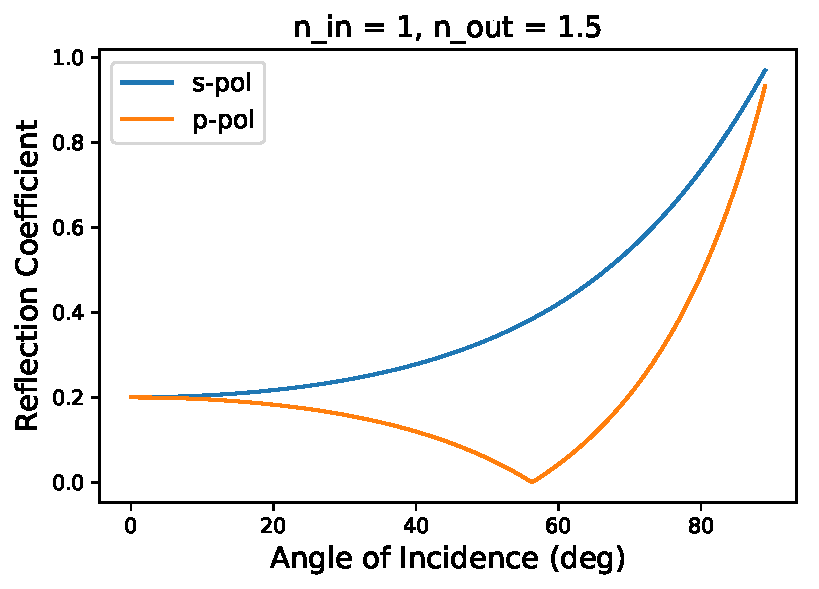
\includegraphics[width=0.45\textwidth]{test_plots/reflection_coeffs_example.pdf}
    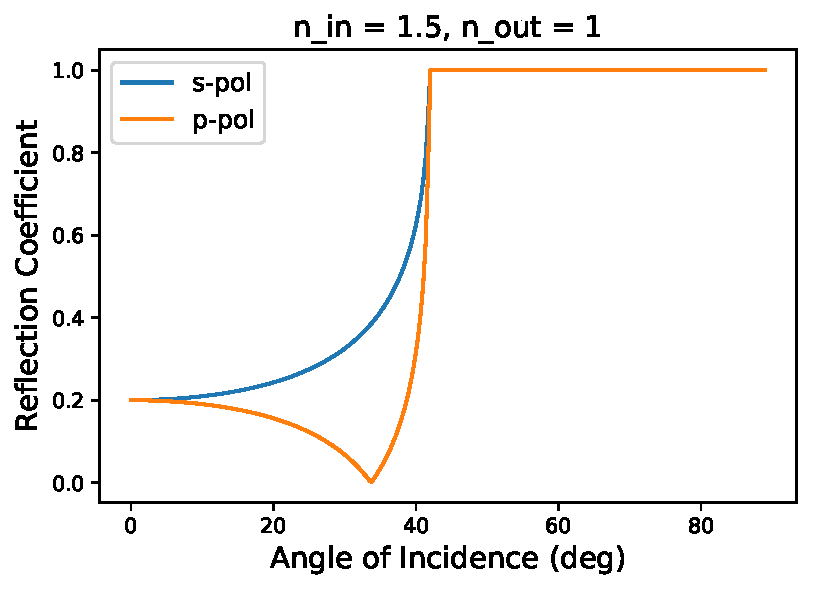
\includegraphics[width=0.45\textwidth]{test_plots/total_internal_reflection_example.pdf}
      \caption{Left: The reflection amplitudes for $s$- and $p$-polarized waves from vacuum incident on an isotropic material with index $n=1.5$. Right: The reflection amplitudes for $s$- and $p$- polarized waves from an isotropic material with index $n=1.5$ incident on vacuum.} \label{fig:brewsterandTIR}
      \end{centering}
\end{figure}




%%%%%%%%%%%%%%%%%%%%%%%%%%%%%%%%%%%%%%%%%%%%%%%%%%%%%%%%%%%%%%%%%%%%%%

\section{Reflection in Arbitrary Medium}
\label{sec:arbitraryREFL}

The real power of \tw{wavecalc} is in its ability to extend our analysis beyond the safety of isotropic media, and dive into the stranger and richer world of general materials. In this example and several to follow, we will model a hypothetical orthorhombic material, which has principal indices $n_x =1.4$, $n_y = 1.9$, and $n_z =2.4$. Though no such real material is known to the author, choosing a highly anisotropic medium makes for more interesting plots.

As a first look at this medium, we test the Law of Reflection. Specifically, for a wave in the medium incident on an interface with the vacuum (for example) with a given incidence angle (as defined by the incident wave-vector), what angles do the reflected wave vectors make with respect to the interface normal? To make things interesting, we will first rotate our medium with respect to the lab coordinates by:
\es
R_z^{-1}(45^\circ)R_y^{-1}(45^\circ)R_x^{-1}(45^\circ) \tens{\mbfg{\ve}} R_x(45^\circ)R_y(45^\circ)R_z(45^\circ)
\ef
\noindent We have rotated the medium by 45 degrees three times, first about the $x$-axis, then about the $y$-axis, and then about $z$. We will also suppose the surface plane is the $x$-$y$ plane, and the incidence plane is the $y$-$z$ plane. Then we can calculate the reflection angles for the $\alpha$- and $\beta$-waves with:
\begin{verbatim}
>> wav = wc.obj.wave()
>> surf = wc.obj.surface()
>> med = wc.obj.medium(epx=1.4**2,epy=1.9**2,epz=2.4**2)
>> med.rotate(45,'x') ; med.rotate(45,'y') ; med.rotate(45,'z')
>> surf = med + surf
>> wav = wav + med
>> thetas = np.linspace(0,60,61)
>> Ang_a = [] ; Ang_b = []
>> for t in thetas:
>>    wav.rotate(t,'x')
>>    wav.fixmode() 
>>    out = wav@surf
>>    out_a = out[0] ; out_b = out[1]
>>    k_a = out_a.kvec ; k_b = out_b.kvec
>>    ang_a = (180/pi)*np.arctan(k_a[1,0]/k_a[2,0])
>>    ang_b = (180/pi)*np.arctan(k_b[1,0]/k_b[2,0])
>>    Ang_a.append(ang_a) ; Ang_b.append(ang_b)
>>    wav.rotate(-t,'x')
>> Ang_a = np.asarray(Ang_a) ; Ang_b = np.asarray(Ang_b)
\end{verbatim}
\noindent We have constructed three arrays: \tw{thetas} which is the list of integers from 0 to 60 inclusive, and both \tw{Ang\_a} \tw{Ang\_b} the lists of corresponding reflection angles for the $\alpha$-wave and $\beta$-wave respectively. To plot this data, we execute:
\begin{verbatim}
>> plt.plot(thetas,Ang_a,label='alpha-wave')
>> plt.plot(thetas,Ang_b,label='beta-wave')
>> plt.plot(thetas,thetas,'k--')
>> plt.title('''Wave vector reflection, y-z incidence plane
>> nx=1.4, ny=1.9, nz=2.4, Rz(45)Ry(45)Rx(45)''',fontsize=14)
>> plt.xlabel("Angle of Incidence (deg)",fontsize=14)
>> plt.ylabel("Angle of Reflection (deg)",fontsize=14)
>> plt.legend(fontsize=12)
>> plt.show()
\end{verbatim}
\noindent The result is shown in Figure \ref{fig:arbREFL}. We see quite clearly that neither the $\alpha$- nor $\beta$-wave obey the rule to which we are so accustomed: the angle of incidence is not the angle of reflection, except for the case of normal incidence.





\begin{figure}[!htb]
  \begin{centering}
    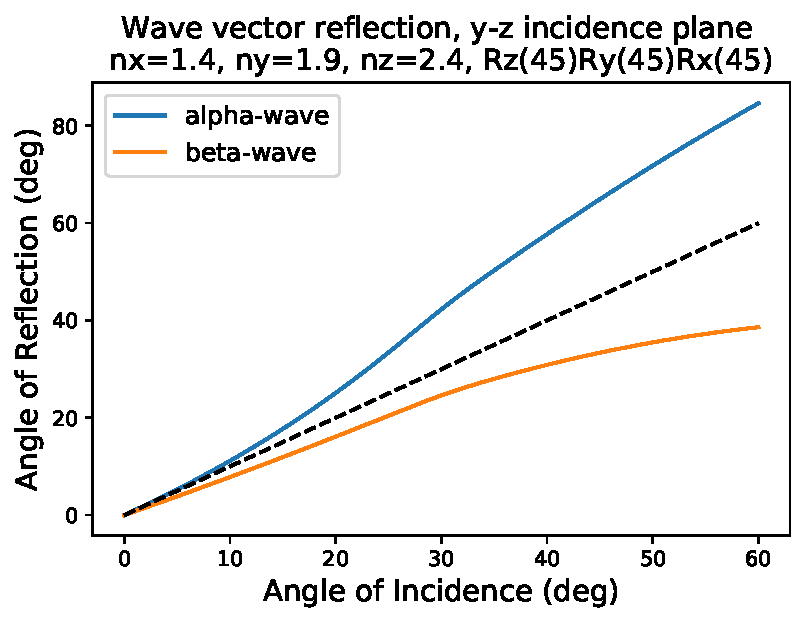
\includegraphics[width=0.6\textwidth]{test_plots/arbitrary_reflection_example.pdf}
        \caption{The angle that the wave vector makes with the incident normal for a given angle of incidence. The $\alpha$-wave is shown in blue and the $\beta$-wave in orange. The dashed black line is the identity.} \label{fig:arbREFL}
      \end{centering}
\end{figure}






%%%%%%%%%%%%%%%%%%%%%%%%%%%%%%%%%%%%%%%%%%%%%%%%%%%%%%%%%%%%%%%%%%%%%%

\section{Poynting Separation in Arbitrary Medium}
\label{sec:arbitraryPOYNTING}

\begin{verbatim}
>> wav = wc.obj.wave()
>> med = wc.obj.medium(epx=1.4**2,epy=1.9**2,epz=2.4**2)
>> med.rotate(45,'x') ; med.rotate(45,'y') ; med.rotate(45,'z')
>> wav = wav + med
>> thetas = np.linspace(0,180,181)
>> S_k_ang_a = [] ; S_k_ang_b = []
>> for t in thetas:
>>    wav_a = copy.deepcopy(wav) ; wav_b = copy.deepcopy(wav)
>>    wav_a.rotate(t,'x') ; wav_b.rotate(t,'x')
>>    wav_a.fixmode(ab=0) ; wav_b.fixmode(ab=1)
>>    S_a = wav_a.poynting(norm=True) ; S_b = wav_b.poynting(norm=True)
>>    k_a = wav_a.kvec ; k_b = wav_b.kvec
>>    k_a = k_a/np.linalg.norm(k_a) ; k_b = k_b/np.linalg.norm(k_b)
>>    S_k_a = (S_a.T @ k_a)[0,0] ; S_k_b = (S_b.T @ k_b)[0,0]
>>    ang_a = (180/pi)*np.arccos(S_k_a).real 
>>    ang_b = (180/pi)*np.arccos(S_k_b).real
>>    S_k_ang_a.append(ang_a) ; S_k_ang_b.append(ang_b)
>> S_k_ang_a = np.asarray(S_k_ang_a)
>> S_k_ang_b = np.asarray(S_k_ang_b)
\end{verbatim}

\begin{verbatim}
>> plt.plot(thetas,S_k_ang_a,label='a-wave')
>> plt.plot(thetas,S_k_ang_b,label='b-wave')
>> plt.title('''Wave vector - Poynting Vector Separation 
>> wave vector in y-z plane 
>> nx=1.4, ny=1.9, nz=2.4, Rz(45)Ry(45)Rx(45)''',fontsize=14)
>> plt.xlabel("Azimuthal wave vector direction (deg)",fontsize=14)
>> plt.ylabel("Separation (deg)",fontsize=14)
>> plt.legend(fontsize=12)
>> plt.show()
\end{verbatim}


\begin{figure}[!htb]
  \begin{centering}
    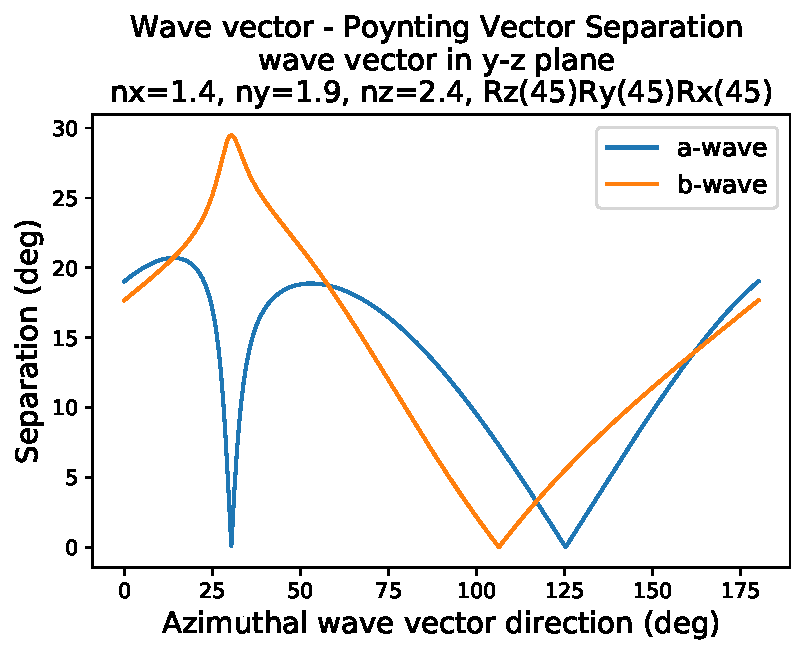
\includegraphics[width=0.6\textwidth]{test_plots/poynting_vec_separation.pdf}
        \caption{} \label{fig:arbPOYNTING}
      \end{centering}
\end{figure}









%%%%%%%%%%%%%%%%%%%%%%%%%%%%%%%%%%%%%%%%%%%%%%%%%%%%%%%%%%%%%%%%%%%%%%

\section{The k-Surface of a Medium}
\label{sec:kspace}
define a function that to find the $a$- and $b$-waves
\begin{verbatim}
>> def example_func(kinit,med,axis,res):
>>    Ka = [] ; Kb = []
>>    for step in range(360//res):
>>        ang = step*res
>>        khat = wc.fun.rotate(kinit,ang,axis)
>>        wav_a = wc.obj.wave(khat,None,med.epsilon)
>>        wav_b = wc.obj.wave(khat,None,med.epsilon)
>>        wav_a.fixmode(ab=0) ; wav_b.fixmode(ab=1)
>>        ka = wav_a.kvec.T ; kb = wav_b.kvec.T
>>        Ka.append(ka.flatten()) ; Kb.append(kb.flatten())
>>    Ka = np.asarray(Ka).real ; Kb = np.asarray(Kb).real
>>    return [Ka,Kb]
\end{verbatim}
build the datasets

\begin{verbatim}
>> med = wc.obj.medium(epx=1.4**2,epy=1.9**2,epz=2.4**2)
>> kinit1 = np.array([[0.,0.,1.]]).T
>> out1 = example_func(kinit1,med,'y',1)
>> X1a = out1[0][:,[0]] ; Z1a = out1[0][:,[2]]
>> X1b = out1[1][:,[0]] ; Z1b = out1[1][:,[2]]
>> kinit2 = np.array([[0.,0.,1.]]).T
>> out2 = example_func(kinit2,med,'x',1)
>> Y2a = out2[0][:,[1]] ; Z2a = out2[0][:,[2]]
>> Y2b = out2[1][:,[1]] ; Z2b = out2[1][:,[2]]
>> kinit3 = np.array([[1.,0.,0.]]).T
>> out3 = example_func(kinit3,med,'z',1)
>> X3a = out3[0][:,[0]] ; Y3a = out3[0][:,[1]]
>> X3b = out3[1][:,[0]] ; Y3b = out3[1][:,[1]]
\end{verbatim}

plot the data
\begin{verbatim}
>> fig = plt.figure(figsize=(15,5))
>> tup1 = [1,X1a,X1b,Z1a,Z1b,'kx','kz','ky=0']
>> tup2 = [2,Y2a,Y2b,Z2a,Z2b,'ky','kz','kx=0']
>> tup3 = [3,X3a,X3b,Y3a,Y3b,'kx','ky','kz=0']
>> tup = (tup1,tup2,tup3)
>> for i,xa,xb,ya,yb,labx,laby,title in tup:
>>    ax = fig.add_subplot(1,3,i)
>>    ax.plot(xa,ya,label='a-wave') ; ax.plot(xb,yb,label='b-wave')
>>    ax.set_xlabel(labx,fontsize=14) ; ax.set_ylabel(laby,fontsize=14)
>>    ax.set_title(title,fontsize=14)
>>    ax.set_xticks([-2,-1,0,1,2]) ; ax.set_yticks([-2,-1,0,1,2])
>>    ax.set_xticks([-2.5,-1.5,-.5,.5,1.5,2.5],minor=True)
>>    ax.set_yticks([-2.5,-1.5,-.5,.5,1.5,2.5],minor=True)
>>    ax.grid(True,which='both')
>> plt.figlegend(fontsize=14,loc='center',bbox_to_anchor=(.93,0.25,.015,1))
>> plt.tight_layout(rect=[0,0,.9,.9])
>> fig.suptitle('k-surface: nx=1.4, ny=1.9, nz=2.4',fontsize=16)
>> plt.show()
\end{verbatim}






\begin{figure}[!htb]
  \begin{centering}
    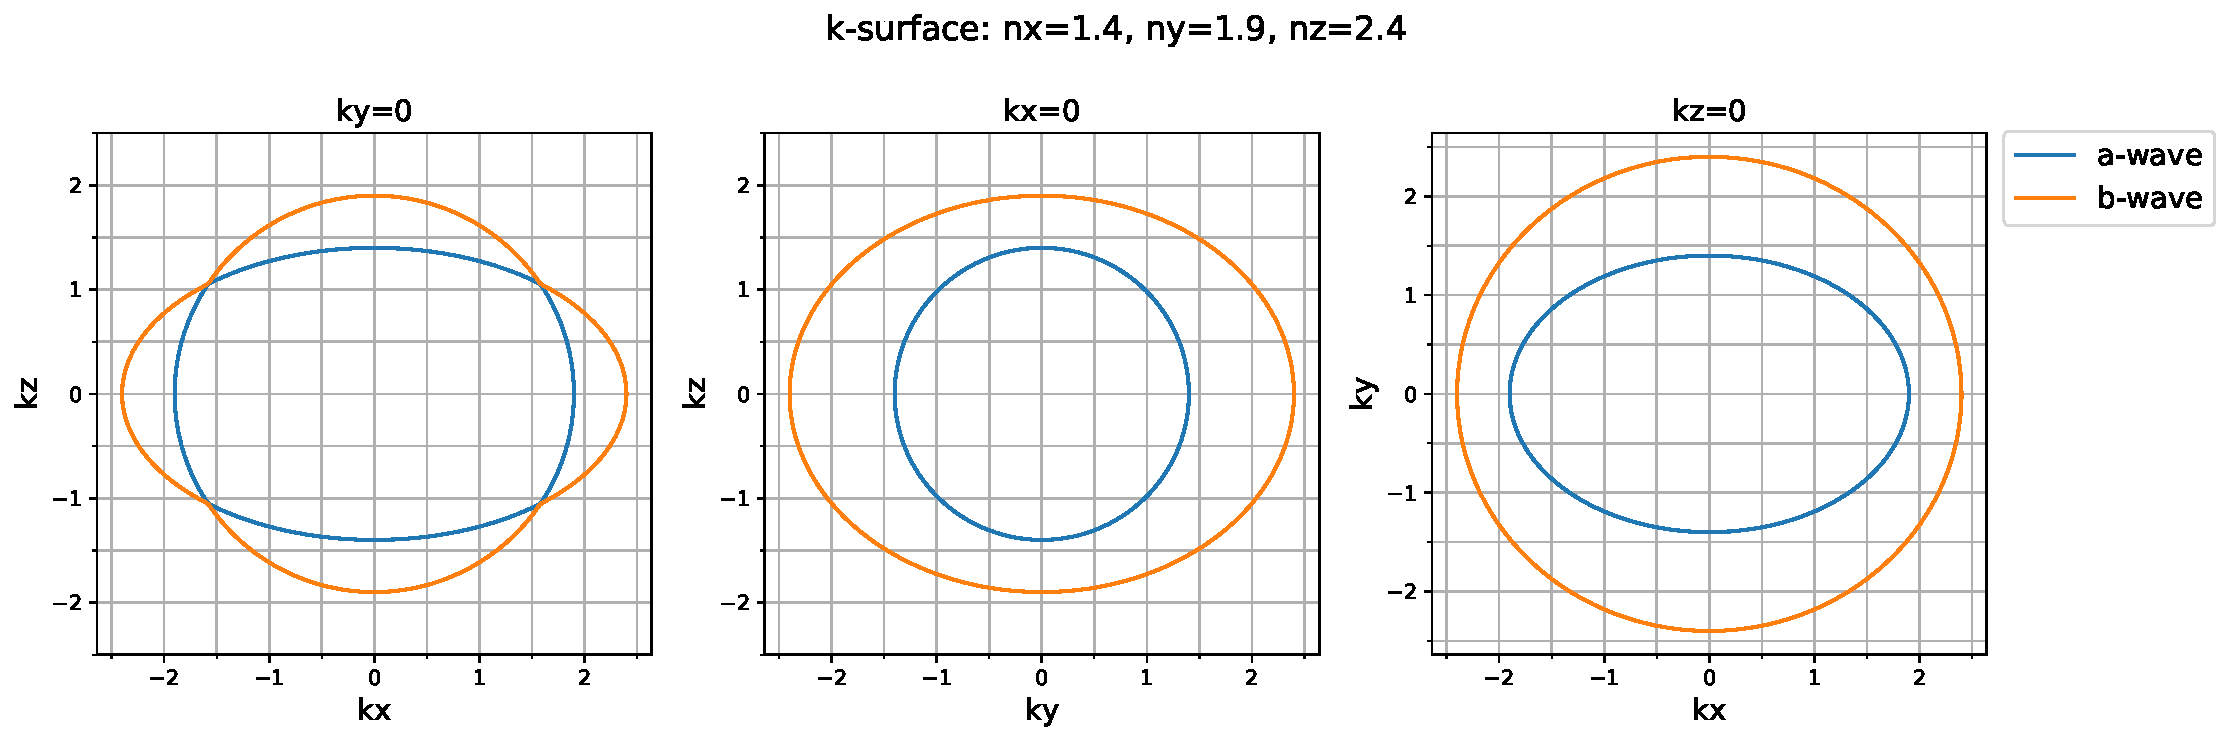
\includegraphics[width=1\textwidth]{test_plots/k_surface_example.pdf}
        \caption{} \label{fig:arbKSURF}
      \end{centering}
\end{figure}








%%%%%%%%%%%%%%%%%%%%%%%%%%%%%%%%%%%%%%%%%%%%%%%%%%%%%%%%%%%%%%%%%%%%%%
%%%%%%%%%%%%%%%%%%%%%%%%%%%%%%%%%%%%%%%%%%%%%%%%%%%%%%%%%%%%%%%%%%%%%%
%%%%%%%%%%%%%%%%%%%%%%%%%%%%%%%%%%%%%%%%%%%%%%%%%%%%%%%%%%%%%%%%%%%%%%
%%%%%%%%%%%%%%%%%%%%%%%%%%%%%%%%%%%%%%%%%%%%%%%%%%%%%%%%%%%%%%%%%%%%%%
%%%%%%%%%%%%%%%%%%%%%%%%%%%%%%%%%%%%%%%%%%%%%%%%%%%%%%%%%%%%%%%%%%%%%%

\chapter{WaveCalc Cheat Sheet}
\label{chap:cheatsheet}

\section{WaveCalc Objects}
\label{sec:objectscheat}

\begin{table}[ht]
\begin{center}
\caption*{\tw{wavecalc.classes.wave(kvec=None, efield=None, phase=None, **kwargs)}}
\begin{tabular}{>{\centering\arraybackslash}m{3.5cm}|>{\centering\arraybackslash}m{3.5cm}|>{\arraybackslash}m{6.5cm}}
\hline
 \textbf{Argument} & \textbf{Type} & \textbf{Details} \\
 \hline
 \tw{kvec} & \tw{numpy.ndarray} & A \tw{(3,1)} array which defines the wavevector of the wave object \\
 \hline
 \tw{efield} & \tw{numpy.ndarray} & A \tw{(3,1)} array which defines the electric field vector of the wave object \\
 \hline
  \tw{phase} & \tw{int}, \tw{float}, \tw{complex} & A value which defines the phase of the wave object \\
 \hline
  \tw{medium} & \tw{numpy.ndarray} & A \tw{(3,3)} array which which defines the medium in which the wave object exists\\
 \hline
 \tw{pol} & \tw{numpy.ndarray} & A \tw{(3,1)} array which defines the polarization of the electric field of the wave object\\
 \hline
  \tw{amp} & \tw{int}, \tw{float}, \tw{complex} & A value which defines the amplitude of the electric field of the wave object \\
 \hline
 \tw{everything} & \tw{bool} & An argument which when set to \tw{False} will instantiate the wave object with all attributes assigned as \tw{None} \\
 \hline
\end{tabular}
%\caption{testing a caption}
\label{tab:wavcheatsheet}
\end{center}
\end{table}


\begin{table}[ht]
\begin{center}
\caption*{\tw{wavecalc.classes.surface(normal=None, **kwargs)}}
\begin{tabular}{>{\centering\arraybackslash}m{3.5cm}|>{\centering\arraybackslash}m{3.5cm}|>{\arraybackslash}m{6.5cm}}
\hline
 \textbf{Argument} & \textbf{Type} & \textbf{Details} \\
 \hline
 \tw{normal} & \tw{numpy.ndarray} & A \tw{(3,1)} array which defines the surface normal vector of the surface object \\
 \hline
 \tw{into} & \tw{numpy.ndarray} & A \tw{(3,3)} array which defines the dielectric tensor of the medium the surface normal points into\\
 \hline
  \tw{out} & \tw{numpy.ndarray} & A \tw{(3,3)} array which defines the dielectric tensor of the medium the surface normal points out of \\
 \hline
  \tw{coat} & \tw{str} & A string which defines the kind of optical coating present on the surface object, either \tw{'HR'} or \tw{'AR'} if specified\\
 \hline
 \tw{everything} & \tw{bool} & An argument which when set to \tw{False} will instantiate the surface object with all attributes assigned as \tw{None} \\
 \hline
\end{tabular}
%\caption{testing a caption}
\label{tab:surfcheatsheet}
\end{center}
\end{table}




\begin{table}[ht]
\begin{center}
\caption*{\tw{wavecalc.classes.medium(epx=None, epy=None, epz=None, **kwargs)}}
\begin{tabular}{>{\centering\arraybackslash}m{3.5cm}|>{\centering\arraybackslash}m{3.5cm}|>{\arraybackslash}m{6.5cm}}
\hline
 \textbf{Argument} & \textbf{Type} & \textbf{Details} \\
 \hline
 \tw{epx} & \tw{int}, \tw{float}, \tw{complex} & A value which  \\
 \hline
 \tw{epy} & \tw{int}, \tw{float}, \tw{complex} & \\
 \hline
  \tw{epz} & \tw{int}, \tw{float}, \tw{complex}&  \\
 \hline
  \tw{ep\_all} & \tw{int}, \tw{float}, \tw{complex} & \\
 \hline
  \tw{epsilon} & \tw{numpy.ndarray} & A \tw{(3,3)} array which defines the dielectric tensor of the medium object \\
 \hline
 \tw{everything} & \tw{bool} & An argument which when set to \tw{False} will instantiate the medium object with all attributes assigned as \tw{None} \\
 \hline
\end{tabular}
%\caption{testing a caption}
\label{tab:medcheatsheet}
\end{center}
\end{table}



%%%%%%%%%%%%%%%%%%%%%%%%%%%%%%%%%%%%%%%%%%%%%%%%%%%%%%%%%%%%%%%%%%%%%%
%%%%%%%%%%%%%%%%%%%%%%%%%%%%%%%%%%%%%%%%%%%%%%%%%%%%%%%%%%%%%%%%%%%%%%
%%%%%%%%%%%%%%%%%%%%%%%%%%%%%%%%%%%%%%%%%%%%%%%%%%%%%%%%%%%%%%%%%%%%%%
%%%%%%%%%%%%%%%%%%%%%%%%%%%%%%%%%%%%%%%%%%%%%%%%%%%%%%%%%%%%%%%%%%%%%%
%%%%%%%%%%%%%%%%%%%%%%%%%%%%%%%%%%%%%%%%%%%%%%%%%%%%%%%%%%%%%%%%%%%%%%

\chapter{The Algebra of WaveCalc: UNDER CONSTRUCTION}
\label{chap:algebra}

If we denote the medium, surface, and wave spaces respectively as $\mathcal{M}$, $\mathcal{S}$, $\mathcal{W}$, then:

Space of 3-dimensional vectors as $\mathcal{V}$, and the space of $3\times 3$ matrices as $\mathcal{A}$

\es
\begin{array}{rcl}
\mathcal{S} &=& \left\{ \mbf{s} =(s_1,s_2, s_3): s_1, s_3 \in \mathcal{A}\mbox{, and } s_2 \in \mathcal{V}  \right\} \\
\mathcal{W}& =& \left\{ \mbf{w}=(w_1,w_2, w_3): w_1, w_2 \in \mathcal{V}\mbox{, and } w_3 \in \mathcal{A}  \right\} \\
\mathcal{M} &=& \left\{ \mbf{m} =(m): m \in \mathcal{A} \right\}
\end{array}
\ef
\noindent For $\mbf{s}=(s_1, s_2, s_3)$, $s_1$ is the \tw{out} attribute, $s_2$ is the \tw{normal} attribute, and $s_3$ is the \tw{into} attribute. For $\mbf{w} = (w_1, w_2,w_3)$, $w_1$ is the \tw{kvec} attribute, $w_2$ is the \tw{efield} attribute, and $w_3$ is the \tw{medium} attribute. Finally, for $\mbf{m}=(m)$, $m$ is the \tw{epsilon} attribute. In this notation, the default attribute assignment is denoted as a 1; for example, a surface with all default  values would be represented as $\mbf{s} = (1,1,1)$. All of the binary addition and subtractions are defined below:
\es \mbox{Yield a surface }
\begin{cases}
&\mbf{m}_a +^1 \mbf{m}_b = (m_a, 1, m_b)  \\
 &\mbf{m}_a -^1 \mbf{m}_b = (m_b, 1, m_a)  \\
 & \mbf{s} +^{2}\mbf{m} = (s_1,s_2, m) \\
 & \mbf{m}+^{3} \mbf{s} = (m,s_2,s_3) \\
 & \mbf{s}-^2\mbf{m} = (m, s_2, s_3) \\
  &\mbf{m}-^3\mbf{s} = (s_1,s_2,m) 
\end{cases} \quad\quad\quad
\mbox{Yield a wave }
\begin{cases}
&\mbf{m} +^4 \mbf{w} = (w_1, w_2, m)  \\
 &\mbf{w} +^5 \mbf{m} = (w_1, w_2, m)  
\end{cases}
\ef
\noindent Where we have used superscripts to remind ourselves that each kind of addition and subtraction is a distinct mapping. From the definitions, many properties immediately follow; for example addition and subtraction over $\mathcal{M}$ are related by:
\es
\mbf{m}_a+^1 \mbf{m}_b = \mbf{m}_b -^1 \mbf{m}_a
\ef
\noindent and similarly:
\es
\mbf{m} +^3\mbf{s} =\mbf{s}-^2\mbf{m} \quad\quad\quad \mbf{m}-^3\mbf{s}=\mbf{s}+^2\mbf{m}
\ef
\noindent These are the analogues of commutation relations in this strange new algebra. The operators over media and surfaces also have an analogue of associativity:
\es
\mbf{m}_a+^3(\mbf{m}_b+^1\mbf{m}_c) = (\mbf{m}_a+^1\mbf{m}_b)+^2\mbf{m}_c \quad\quad\quad
\mbf{m}_a-^3(\mbf{m}_b-^1\mbf{m}_c) = (\mbf{m}_a-^1\mbf{m}_b)-^2\mbf{m}_c
\label{eq:associkindof}
\ef
\noindent however, one should be careful when attempting to generalize. It could be tempting to drop the superscripts and parentheses from (\ref{eq:associkindof}), but take note that the order of additions matter. In particular, if we have a series of media:
\es
\mbf{m}_1 + \mbf{m}_2+ \mbf{m}_3 + \cdots+ \mbf{m}_{n-2} + \mbf{m}_{n-1}+ \mbf{m}_n
\nonumber
\ef
\noindent the only meaningful ordering of operations is for the first evaluated sum to be $+^1$, and then every addition on the right side is $+^2$, and on the left side is $+^3$. A similar conclusion is true for subtraction, with $-^1$ playing the role of $+^1$, $-^2$ playing the role of $+^2$, and $-^3$ the role of $+^3$. 

We will prove that this is true for the case of addition. Suppose we have a series of $n$ media being added together, it immediately follows that there are $n-1$ addition operations in the expression of the series, which we number from left to right. Consider the first addition operation to be evaluated, we know two things about this addition: first, that it is an addition between two media, and so must be $+^1$, and second, that its order in the series, $k$, must satisfy $1\leq k \leq n-1$. Suppose now, for the purpose of proof by contradiction, that at least one of three conditions hold true: 1) there is and addition operator $+^2$ with order $m<k$, 2) there is an addition operator $+^3$ with order $p>k$, or 3) there is and addition operator $+^1$ with order $q \neq k$. In the first case, we know that because $+^2$ adds surfaces on the left to media on the right, there must then be a surface object to the left of $\mbf{m}_k$. In the second case, we know that because $+^3$ adds media on the left to surfaces on the right, there must be a surface to the right of $\mbf{m}_{k+1}$. However, $\mbf{m}_k +^1 \mbf{m}_{k+1}$ is the first evaluated operation and results in a surface, and all subsequent additions with media will only result in new surfaces.


 We will call these expressions well-ordered. With this knowledge, for any well ordered sums and differences of elements of $\mathcal{M}$, the following is true:
\es
\mbf{m}_1 \pm \mbf{m}_2 \pm \mbf{m}_3 \pm \cdots \pm \mbf{m}_{n-2} \pm \mbf{m}_{n-1}\pm \mbf{m}_n = \mbf{m}_1 \pm\mbf{m}_{n}
\ef 



\es \mbox{Unary operations }
\begin{cases}
&-\mbf{s} = (s_1, -s_2, s_3)  \\
 &\sim\mbf{s}  = (s_3, s_2, s_1) \\
 & - \mbf{w} = (-w_1,-w_2,w_3)  
\end{cases}
\ef

\es
\mbf{m} - (\sim \mbf{s}) = \sim(\mbf{m}+\mbf{s})
\ef



\es
\mbf{m} = (m) \in\mathcal{S}
\ef
\es
\mbf{w} = () \in \mathcal{W}
\ef
\es
1
\ef

\es
\begin{array}{cccl}
& \mathcal{M}\times \mathcal{M} & \to & \mathcal{S} \\
&\mathcal{M}\times\mathcal{S} & \to & \mathcal{S} \\
&\mathcal{S}\times\mathcal{M} & \to & \mathcal{S} \\
+: & \mathcal{M} \times \mathcal{W} & \to & \mathcal{W} \\
& \mathcal{W}\times\mathcal{M} & \to & \mathcal{W} \\
& \mathcal{S}\times\mathcal{W} & \to & \mathcal{W}\times \mathcal{W} \\
& \mathcal{W}\times \mathcal{S} & \to & \mathcal{W}\times \mathcal{W}
\end{array} \quad\quad\quad\quad
\begin{array}{cccl}
& \mathcal{M}\times \mathcal{M} & \to & \mathcal{S} \\
&\mathcal{M}\times\mathcal{S} & \to & \mathcal{S} \\
&\mathcal{S}\times\mathcal{M} & \to & \mathcal{S} \\
-: & \mathcal{S}\times\mathcal{W} & \to & \mathcal{W}\times \mathcal{W} \\
& \mathcal{W}\times \mathcal{S} & \to & \mathcal{W}\times \mathcal{W} \\
& \mathcal{S}  & \to & \mathcal{S} \\
& \mathcal{W} & \to & \mathcal{W}
\end{array}
\ef

\es
\mbf{m}_1 + \mbf{m}_2 = (m_1, 1, m_2) \in \mathcal{S}
\ef

\es
\mbf{m}_1 - \mbf{m}_2 = (m_2, 1, m_1) \in \mathcal{S}
\ef

\es
\mbf{m}_1 + 
\ef

\es
m_1 + m_2 + m_3 = m_1 + m_3
\ef

\es
m_1 - m_2 - m_3 = 
\ef

\es
o_1 + o_2 = o_2 - o_1
\ef


We can best summarize the properties of addition and subtraction by considering three arbitrary WaveCalc objects, $o_1$, $o_2$, and $o_3$, of which at least two are media, none are waves, and no more than one is a surface. Then addition and subtraction are both associative:
\es
\begin{array}{l}
o_1 + (o_2 + o_3) = (o_1 + o_2) + o_3 \\
o_1 - (o_2 - o_3) = (o_1 - o_2) - o_3
\end{array}
\ef
\noindent they are anti-commutative in the sense that:
\es
o_1 + o_2 = o_2 - o_1
\ef
\noindent and they are collapsible in the sense that:
\es
\begin{array}{l}
o_1 +o_2 +o_3 = o_1 + o_3 \\
o_1 - o_2 - o_3 =o_1 - o_3
\end{array}
\ef
\noindent so long as $o_2$ is not a surface. Notice that while addition and subtraction are associative, they are not mutually associative. To illustrate this we take the two quantities:
\es
o_1 - (o_2+o_3) \quad \quad\quad \quad (o_1 -o_2) + o_3
\nonumber
\ef
\noindent and write them in double addition form:
\es
\begin{array}{l}
o_1 - (o_2 + o_3) = o_2 +o_3 + o_1  \\
(o_1 - o_2) + o_3 = o_2 +o_1 + o_3
\end{array}
\label{eq:nomutassoc}
\ef
\noindent As addition is not commutative, in general the objects $o_3+o_1$ and $o_1 + o_3$ will be distinct, and so too will be the sums in (\ref{eq:nomutassoc}).





















%%%%%%%%%%%%%%%%%%%%%%%%%%%%%%%%%%%%%%%%%%%%%%%%%%%%%%%%%%%%%%%%%%%%%%
%%%%%%%%%%%%%%%%%%%%%%%%%%%%%%%%%%%%%%%%%%%%%%%%%%%%%%%%%%%%%%%%%%%%%%
%%%%%%%%%%%%%%%%%%%%%%%%%%%%%%%%%%%%%%%%%%%%%%%%%%%%%%%%%%%%%%%%%%%%%%
%%%%%%%%%%%%%%%%%%%%%%%%%%%%%%%%%%%%%%%%%%%%%%%%%%%%%%%%%%%%%%%%%%%%%%
%%%%%%%%%%%%%%%%%%%%%%%%%%%%%%%%%%%%%%%%%%%%%%%%%%%%%%%%%%%%%%%%%%%%%%

\chapter{Notes on Future Development}
\label{chap:scratch}



\noindent Things that need further development in this document:
\begin{itemize}
\item optic axes section should be developed
\item the quartic paradox needs to be explained and addressed
\item how to treat AR or HR coatings theoretically should be addressed
\item the overloaded unary operations need to be explained
\item the algebra chapter needs to be completed
\item the modes section of the implementation chapter needs to be written, even though it's boring
\end{itemize}


\noindent Things that need further development and implementation in \tw{wavecalc}:
\begin{itemize}
\item handling of evanescent waves needs to be addressed
\item \tw{aux\_rotate\_copy} needs to only rotate attributes that are not Nonetype
\item \tw{clean} method must be revised
\item \tw{aux\_remove\_vacuum} needs to be developed and interfaced with \tw{aux\_waveinterf} to get rid of modes with no electric field amplitude
\item chaining surfaces together and appropriately tracking waves
\end{itemize}

\noindent Things I might like to implement in the future:
\begin{itemize}
\item Include a unique identifier in the outputs of main functions that is only dependent on the other outputs. This would allow a quick way to verify that a change to the code has not changed the outputs of main functions. Making it actually unique would be difficult, but if the identifier is, for example, a very large number, it could be made effectively unique. 
\item A coating class for custom-property coatings. This would require an overhaul of the coating handling.
\item Better handling of numerical errors
\item Better handling of complex wave vectors
\item Add a module for \tw{wavecalc} specific exceptions
\item Add some notion of physical extent and phase so that interference phenomenon can be directly investigated
\item Include more documentation on how functions handle the calculations so that the user might better understand errors
\end{itemize}
















\end{document}

















%%%%%%%%%%%%%%%%%%%%%%%%%%%%%%%%%%%%%%%%%%%%%%%%%%%%%%%%
%%%%%%%%%%%%%%%%%%%%%%%%%%%%%%%%%%%%%%%%%%%%%%%%%%%%%%%%
%%%%%%%%%%%%%%%%%%%%%%%%%%%%%%%%%%%%%%%%%%%%%%%%%%%%%%%%
%%%%%%%%%%%%%%%%%%%%%%%%%%%%%%%%%%%%%%%%%%%%%%%%%%%%%%%%
%%%%%%%%%%%%%%%%%%%%%%%%%%%%%%%%%%%%%%%%%%%%%%%%%%%%%%%%
%%%%%%%%%%%%%%%%%%%%%%%%%%%%%%%%%%%%%%%%%%%%%%%%%%%%%%%%
%%%%%%%%%%%%%%%%%%%%%%%%%%%%%%%%%%%%%%%%%%%%%%%%%%%%%%%%
%%%%%%%%%%%%%%%%%%%%%%%%%%%%%%%%%%%%%%%%%%%%%%%%%%%%%%%%
%%%%%%%%%%%%%%%%%%%%%%%%%%%%%%%%%%%%%%%%%%%%%%%%%%%%%%%%
%%%%%%%%%%%%%%%%%%%%%%%%%%%%%%%%%%%%%%%%%%%%%%%%%%%%%%%%
%%%%%%%%%%%%%%%%%%%%%%%%%%%%%%%%%%%%%%%%%%%%%%%%%%%%%%%%
%%%%%%%%%%%%%%%%%%%%%%%%%%%%%%%%%%%%%%%%%%%%%%%%%%%%%%%%
%%%%%%%%%%%%%%%%%%%%%%%%%%%%%%%%%%%%%%%%%%%%%%%%%%%%%%%%
%%%%%%%%%%%%%%%%%%%%%%%%%%%%%%%%%%%%%%%%%%%%%%%%%%%%%%%%
%%%%%%%%%%%%%%%%%%%%%%%%%%%%%%%%%%%%%%%%%%%%%%%%%%%%%%%%
%%%%%%%%%%%%%%%%%%%%%%%%%%%%%%%%%%%%%%%%%%%%%%%%%%%%%%%%
%%%%%%%%%%%%%%%%%%%%%%%%%%%%%%%%%%%%%%%%%%%%%%%%%%%%%%%%
%%%%%%%%%%%%%%%%%%%%%%%%%%%%%%%%%%%%%%%%%%%%%%%%%%%%%%%%
%%%%%%%%%%%%%%%%%%%%%%%%%%%%%%%%%%%%%%%%%%%%%%%%%%%%%%%%
%%%%%%%%%%%%%%%%%%%%%%%%%%%%%%%%%%%%%%%%%%%%%%%%%%%%%%%%
%%%%%%%%%%%%%%%%%%%%%%%%%%%%%%%%%%%%%%%%%%%%%%%%%%%%%%%%
%%%%%%%%%%%%%%%%%%%%%%%%%%%%%%%%%%%%%%%%%%%%%%%%%%%%%%%%
%%%%%%%%%%%%%%%%%%%%%%%%%%%%%%%%%%%%%%%%%%%%%%%%%%%%%%%%
%%%%%%%%%%%%%%%%%%%%%%%%%%%%%%%%%%%%%%%%%%%%%%%%%%%%%%%%
%%%%%%%%%%%%%%%%%%%%%%%%%%%%%%%%%%%%%%%%%%%%%%%%%%%%%%%%
%%%%%%%%%%%%%%%%%%%%%%%%%%%%%%%%%%%%%%%%%%%%%%%%%%%%%%%%
%%%%%%%%%%%%%%%%%%%%%%%%%%%%%%%%%%%%%%%%%%%%%%%%%%%%%%%%
%%%%%%%%%%%%%%%%%%%%%%%%%%%%%%%%%%%%%%%%%%%%%%%%%%%%%%%%
%%%%%%%%%%%%%%%%%%%%%%%%%%%%%%%%%%%%%%%%%%%%%%%%%%%%%%%%
%%%%%%%%%%%%%%%%%%%%%%%%%%%%%%%%%%%%%%%%%%%%%%%%%%%%%%%%
%%%%%%%%%%%%%%%%%%%%%%%%%%%%%%%%%%%%%%%%%%%%%%%%%%%%%%%%
%%%%%%%%%%%%%%%%%%%%%%%%%%%%%%%%%%%%%%%%%%%%%%%%%%%%%%%%
%%%%%%%%%%%%%%%%%%%%%%%%%%%%%%%%%%%%%%%%%%%%%%%%%%%%%%%%
%%%%%%%%%%%%%%%%%%%%%%%%%%%%%%%%%%%%%%%%%%%%%%%%%%%%%%%%
%%%%%%%%%%%%%%%%%%%%%%%%%%%%%%%%%%%%%%%%%%%%%%%%%%%%%%%%
%%%%%%%%%%%%%%%%%%%%%%%%%%%%%%%%%%%%%%%%%%%%%%%%%%%%%%%%
%%%%%%%%%%%%%%%%%%%%%%%%%%%%%%%%%%%%%%%%%%%%%%%%%%%%%%%%
%%%%%%%%%%%%%%%%%%%%%%%%%%%%%%%%%%%%%%%%%%%%%%%%%%%%%%%%
%%%%%%%%%%%%%%%%%%%%%%%%%%%%%%%%%%%%%%%%%%%%%%%%%%%%%%%%
%%%%%%%%%%%%%%%%%%%%%%%%%%%%%%%%%%%%%%%%%%%%%%%%%%%%%%%%
%%%%%%%%%%%%%%%%%%%%%%%%%%%%%%%%%%%%%%%%%%%%%%%%%%%%%%%%
%%%%%%%%%%%%%%%%%%%%%%%%%%%%%%%%%%%%%%%%%%%%%%%%%%%%%%%%
%%%%%%%%%%%%%%%%%%%%%%%%%%%%%%%%%%%%%%%%%%%%%%%%%%%%%%%%
%%%%%%%%%%%%%%%%%%%%%%%%%%%%%%%%%%%%%%%%%%%%%%%%%%%%%%%%
%%%%%%%%%%%%%%%%%%%%%%%%%%%%%%%%%%%%%%%%%%%%%%%%%%%%%%%%
%%%%%%%%%%%%%%%%%%%%%%%%%%%%%%%%%%%%%%%%%%%%%%%%%%%%%%%%
%%%%%%%%%%%%%%%%%%%%%%%%%%%%%%%%%%%%%%%%%%%%%%%%%%%%%%%%
%%%%%%%%%%%%%%%%%%%%%%%%%%%%%%%%%%%%%%%%%%%%%%%%%%%%%%%%
%%%%%%%%%%%%%%%%%%%%%%%%%%%%%%%%%%%%%%%%%%%%%%%%%%%%%%%%
%%%%%%%%%%%%%%%%%%%%%%%%%%%%%%%%%%%%%%%%%%%%%%%%%%%%%%%%
%%%%%%%%%%%%%%%%%%%%%%%%%%%%%%%%%%%%%%%%%%%%%%%%%%%%%%%%
%%%%%%%%%%%%%%%%%%%%%%%%%%%%%%%%%%%%%%%%%%%%%%%%%%%%%%%%
%%%%%%%%%%%%%%%%%%%%%%%%%%%%%%%%%%%%%%%%%%%%%%%%%%%%%%%%
%%%%%%%%%%%%%%%%%%%%%%%%%%%%%%%%%%%%%%%%%%%%%%%%%%%%%%%%
%%%%%%%%%%%%%%%%%%%%%%%%%%%%%%%%%%%%%%%%%%%%%%%%%%%%%%%%
%%%%%%%%%%%%%%%%%%%%%%%%%%%%%%%%%%%%%%%%%%%%%%%%%%%%%%%%
%%%%%%%%%%%%%%%%%%%%%%%%%%%%%%%%%%%%%%%%%%%%%%%%%%%%%%%%
%%%%%%%%%%%%%%%%%%%%%%%%%%%%%%%%%%%%%%%%%%%%%%%%%%%%%%%%
%%%%%%%%%%%%%%%%%%%%%%%%%%%%%%%%%%%%%%%%%%%%%%%%%%%%%%%%
%%%%%%%%%%%%%%%%%%%%%%%%%%%%%%%%%%%%%%%%%%%%%%%%%%%%%%%%
%%%%%%%%%%%%%%%%%%%%%%%%%%%%%%%%%%%%%%%%%%%%%%%%%%%%%%%%
%%%%%%%%%%%%%%%%%%%%%%%%%%%%%%%%%%%%%%%%%%%%%%%%%%%%%%%%
%%%%%%%%%%%%%%%%%%%%%%%%%%%%%%%%%%%%%%%%%%%%%%%%%%%%%%%%
%%%%%%%%%%%%%%%%%%%%%%%%%%%%%%%%%%%%%%%%%%%%%%%%%%%%%%%%
%%%%%%%%%%%%%%%%%%%%%%%%%%%%%%%%%%%%%%%%%%%%%%%%%%%%%%%%
%%%%%%%%%%%%%%%%%%%%%%%%%%%%%%%%%%%%%%%%%%%%%%%%%%%%%%%%
%%%%%%%%%%%%%%%%%%%%%%%%%%%%%%%%%%%%%%%%%%%%%%%%%%%%%%%%
%%%%%%%%%%%%%%%%%%%%%%%%%%%%%%%%%%%%%%%%%%%%%%%%%%%%%%%%
%%%%%%%%%%%%%%%%%%%%%%%%%%%%%%%%%%%%%%%%%%%%%%%%%%%%%%%%
%%%%%%%%%%%%%%%%%%%%%%%%%%%%%%%%%%%%%%%%%%%%%%%%%%%%%%%%
%%%%%%%%%%%%%%%%%%%%%%%%%%%%%%%%%%%%%%%%%%%%%%%%%%%%%%%%
%%%%%%%%%%%%%%%%%%%%%%%%%%%%%%%%%%%%%%%%%%%%%%%%%%%%%%%%
%%%%%%%%%%%%%%%%%%%%%%%%%%%%%%%%%%%%%%%%%%%%%%%%%%%%%%%%
%%%%%%%%%%%%%%%%%%%%%%%%%%%%%%%%%%%%%%%%%%%%%%%%%%%%%%%%
%%%%%%%%%%%%%%%%%%%%%%%%%%%%%%%%%%%%%%%%%%%%%%%%%%%%%%%%
%%%%%%%%%%%%%%%%%%%%%%%%%%%%%%%%%%%%%%%%%%%%%%%%%%%%%%%%
%%%%%%%%%%%%%%%%%%%%%%%%%%%%%%%%%%%%%%%%%%%%%%%%%%%%%%%%
%%%%%%%%%%%%%%%%%%%%%%%%%%%%%%%%%%%%%%%%%%%%%%%%%%%%%%%%
%%%%%%%%%%%%%%%%%%%%%%%%%%%%%%%%%%%%%%%%%%%%%%%%%%%%%%%%
%%%%%%%%%%%%%%%%%%%%%%%%%%%%%%%%%%%%%%%%%%%%%%%%%%%%%%%%
%%%%%%%%%%%%%%%%%%%%%%%%%%%%%%%%%%%%%%%%%%%%%%%%%%%%%%%%
%%%%%%%%%%%%%%%%%%%%%%%%%%%%%%%%%%%%%%%%%%%%%%%%%%%%%%%%
%%%%%%%%%%%%%%%%%%%%%%%%%%%%%%%%%%%%%%%%%%%%%%%%%%%%%%%%
%%%%%%%%%%%%%%%%%%%%%%%%%%%%%%%%%%%%%%%%%%%%%%%%%%%%%%%%
%%%%%%%%%%%%%%%%%%%%%%%%%%%%%%%%%%%%%%%%%%%%%%%%%%%%%%%%
%%%%%%%%%%%%%%%%%%%%%%%%%%%%%%%%%%%%%%%%%%%%%%%%%%%%%%%%
%%%%%%%%%%%%%%%%%%%%%%%%%%%%%%%%%%%%%%%%%%%%%%%%%%%%%%%%
%%%%%%%%%%%%%%%%%%%%%%%%%%%%%%%%%%%%%%%%%%%%%%%%%%%%%%%%
%%%%%%%%%%%%%%%%%%%%%%%%%%%%%%%%%%%%%%%%%%%%%%%%%%%%%%%%
%%%%%%%%%%%%%%%%%%%%%%%%%%%%%%%%%%%%%%%%%%%%%%%%%%%%%%%%
%%%%%%%%%%%%%%%%%%%%%%%%%%%%%%%%%%%%%%%%%%%%%%%%%%%%%%%%
%%%%%%%%%%%%%%%%%%%%%%%%%%%%%%%%%%%%%%%%%%%%%%%%%%%%%%%%
%%%%%%%%%%%%%%%%%%%%%%%%%%%%%%%%%%%%%%%%%%%%%%%%%%%%%%%%
%%%%%%%%%%%%%%%%%%%%%%%%%%%%%%%%%%%%%%%%%%%%%%%%%%%%%%%%
%%%%%%%%%%%%%%%%%%%%%%%%%%%%%%%%%%%%%%%%%%%%%%%%%%%%%%%%
%%%%%%%%%%%%%%%%%%%%%%%%%%%%%%%%%%%%%%%%%%%%%%%%%%%%%%%%
%%%%%%%%%%%%%%%%%%%%%%%%%%%%%%%%%%%%%%%%%%%%%%%%%%%%%%%%
%%%%%%%%%%%%%%%%%%%%%%%%%%%%%%%%%%%%%%%%%%%%%%%%%%%%%%%%
%%%%%%%%%%%%%%%%%%%%%%%%%%%%%%%%%%%%%%%%%%%%%%%%%%%%%%%%
%%%%%%%%%%%%%%%%%%%%%%%%%%%%%%%%%%%%%%%%%%%%%%%%%%%%%%%%
%%%%%%%%%%%%%%%%%%%%%%%%%%%%%%%%%%%%%%%%%%%%%%%%%%%%%%%%
%%%%%%%%%%%%%%%%%%%%%%%%%%%%%%%%%%%%%%%%%%%%%%%%%%%%%%%%
%%%%%%%%%%%%%%%%%%%%%%%%%%%%%%%%%%%%%%%%%%%%%%%%%%%%%%%%
%%%%%%%%%%%%%%%%%%%%%%%%%%%%%%%%%%%%%%%%%%%%%%%%%%%%%%%%
%%%%%%%%%%%%%%%%%%%%%%%%%%%%%%%%%%%%%%%%%%%%%%%%%%%%%%%%
%%%%%%%%%%%%%%%%%%%%%%%%%%%%%%%%%%%%%%%%%%%%%%%%%%%%%%%%
%%%%%%%%%%%%%%%%%%%%%%%%%%%%%%%%%%%%%%%%%%%%%%%%%%%%%%%%
%%%%%%%%%%%%%%%%%%%%%%%%%%%%%%%%%%%%%%%%%%%%%%%%%%%%%%%%
%%%%%%%%%%%%%%%%%%%%%%%%%%%%%%%%%%%%%%%%%%%%%%%%%%%%%%%%
%%%%%%%%%%%%%%%%%%%%%%%%%%%%%%%%%%%%%%%%%%%%%%%%%%%%%%%%
%%%%%%%%%%%%%%%%%%%%%%%%%%%%%%%%%%%%%%%%%%%%%%%%%%%%%%%%
%%%%%%%%%%%%%%%%%%%%%%%%%%%%%%%%%%%%%%%%%%%%%%%%%%%%%%%%
%%%%%%%%%%%%%%%%%%%%%%%%%%%%%%%%%%%%%%%%%%%%%%%%%%%%%%%%
%%%%%%%%%%%%%%%%%%%%%%%%%%%%%%%%%%%%%%%%%%%%%%%%%%%%%%%%
%%%%%%%%%%%%%%%%%%%%%%%%%%%%%%%%%%%%%%%%%%%%%%%%%%%%%%%%
%%%%%%%%%%%%%%%%%%%%%%%%%%%%%%%%%%%%%%%%%%%%%%%%%%%%%%%%
%%%%%%%%%%%%%%%%%%%%%%%%%%%%%%%%%%%%%%%%%%%%%%%%%%%%%%%%
%%%%%%%%%%%%%%%%%%%%%%%%%%%%%%%%%%%%%%%%%%%%%%%%%%%%%%%%
%%%%%%%%%%%%%%%%%%%%%%%%%%%%%%%%%%%%%%%%%%%%%%%%%%%%%%%%
%%%%%%%%%%%%%%%%%%%%%%%%%%%%%%%%%%%%%%%%%%%%%%%%%%%%%%%%
%%%%%%%%%%%%%%%%%%%%%%%%%%%%%%%%%%%%%%%%%%%%%%%%%%%%%%%%
%%%%%%%%%%%%%%%%%%%%%%%%%%%%%%%%%%%%%%%%%%%%%%%%%%%%%%%%
%%%%%%%%%%%%%%%%%%%%%%%%%%%%%%%%%%%%%%%%%%%%%%%%%%%%%%%%
%%%%%%%%%%%%%%%%%%%%%%%%%%%%%%%%%%%%%%%%%%%%%%%%%%%%%%%%
%%%%%%%%%%%%%%%%%%%%%%%%%%%%%%%%%%%%%%%%%%%%%%%%%%%%%%%%
%%%%%%%%%%%%%%%%%%%%%%%%%%%%%%%%%%%%%%%%%%%%%%%%%%%%%%%%
%%%%%%%%%%%%%%%%%%%%%%%%%%%%%%%%%%%%%%%%%%%%%%%%%%%%%%%%
%%%%%%%%%%%%%%%%%%%%%%%%%%%%%%%%%%%%%%%%%%%%%%%%%%%%%%%%
%%%%%%%%%%%%%%%%%%%%%%%%%%%%%%%%%%%%%%%%%%%%%%%%%%%%%%%%
%%%%%%%%%%%%%%%%%%%%%%%%%%%%%%%%%%%%%%%%%%%%%%%%%%%%%%%%
%%%%%%%%%%%%%%%%%%%%%%%%%%%%%%%%%%%%%%%%%%%%%%%%%%%%%%%%
%%%%%%%%%%%%%%%%%%%%%%%%%%%%%%%%%%%%%%%%%%%%%%%%%%%%%%%%
%%%%%%%%%%%%%%%%%%%%%%%%%%%%%%%%%%%%%%%%%%%%%%%%%%%%%%%%
%%%%%%%%%%%%%%%%%%%%%%%%%%%%%%%%%%%%%%%%%%%%%%%%%%%%%%%%
%%%%%%%%%%%%%%%%%%%%%%%%%%%%%%%%%%%%%%%%%%%%%%%%%%%%%%%%
%%%%%%%%%%%%%%%%%%%%%%%%%%%%%%%%%%%%%%%%%%%%%%%%%%%%%%%%
%%%%%%%%%%%%%%%%%%%%%%%%%%%%%%%%%%%%%%%%%%%%%%%%%%%%%%%%
%%%%%%%%%%%%%%%%%%%%%%%%%%%%%%%%%%%%%%%%%%%%%%%%%%%%%%%%
%%%%%%%%%%%%%%%%%%%%%%%%%%%%%%%%%%%%%%%%%%%%%%%%%%%%%%%%
%%%%%%%%%%%%%%%%%%%%%%%%%%%%%%%%%%%%%%%%%%%%%%%%%%%%%%%%
%%%%%%%%%%%%%%%%%%%%%%%%%%%%%%%%%%%%%%%%%%%%%%%%%%%%%%%%
%%%%%%%%%%%%%%%%%%%%%%%%%%%%%%%%%%%%%%%%%%%%%%%%%%%%%%%%
%%%%%%%%%%%%%%%%%%%%%%%%%%%%%%%%%%%%%%%%%%%%%%%%%%%%%%%%
%%%%%%%%%%%%%%%%%%%%%%%%%%%%%%%%%%%%%%%%%%%%%%%%%%%%%%%%
%%%%%%%%%%%%%%%%%%%%%%%%%%%%%%%%%%%%%%%%%%%%%%%%%%%%%%%%
%%%%%%%%%%%%%%%%%%%%%%%%%%%%%%%%%%%%%%%%%%%%%%%%%%%%%%%%
%%%%%%%%%%%%%%%%%%%%%%%%%%%%%%%%%%%%%%%%%%%%%%%%%%%%%%%%
%%%%%%%%%%%%%%%%%%%%%%%%%%%%%%%%%%%%%%%%%%%%%%%%%%%%%%%%
%%%%%%%%%%%%%%%%%%%%%%%%%%%%%%%%%%%%%%%%%%%%%%%%%%%%%%%%
%%%%%%%%%%%%%%%%%%%%%%%%%%%%%%%%%%%%%%%%%%%%%%%%%%%%%%%%

%%%%%%%%%%%%%%%%%%%%%%%%%%%%%%%%%%%%%%%%%%%%%%%%%%%%%%%%%%%%%%%%%%%%%%

\chapter{The Wave Calculator Package}
\label{chap:wavecalcpack}

%The wave calculator tool has been coded in Python and packaged as \tw{wavecalc}.

The implementations outlined in Chapter \ref{chap:implement} have been coded in Python and packaged as \tw{wavecalc}. This package provides tools for easily calculating plane wave behavior in dielectric media and at the interface of media. Both as attributes, function arguments, and core functions, WaveCalc relies heavily on objects from the \tw{numpy} package; and so this package is a dependency for \tw{wavecalc}.

In this chapter we will use example code to illustrate the properties and functionality of the \tw{wavecalc} package. In doing so, we use the convention that any line beginning with \verb|>>| is input code, and any line or lines not preceded by a symbol is an output of the input code:
\begin{verbatim}

>> input code
output of code

\end{verbatim}

Technically, in Python everything is an object, however it makes sense to distinguish between the Python objects which are representative of physical entities and the Python objects which are representative of physical processes. The former we refer to as objects, and the latter as functions. Chapter \ref{chap:wavecalcobj} introduces these WaveCalc objects, Chapter \ref{chap:methods} explains the methods associated with these objects, and Chapter \ref{chap:wavecalcfun} describes the primary set of WaveCalc functions. In Chapter \ref{chap:examp}, we will demonstrate the utility of WaveCalc with some examples.

To work with WaveCalc and follow along with the example code, the user will need to import both the \tw{wavecalc} and \tw{numpy} packages into their Python interpreter:
\begin{verbatim}

>> import wavecalc
>> import numpy

\end{verbatim}










Required as inputs:
\begin{itemize}
\item incident $\mbf{k}$
\item the surface normal in the laboratory frame, $\mbfh{s}$
\item 
\end{itemize}


Basic steps:
\begin{itemize}
\item incident wave as $\mbf{E}_0$ and $\mbf{k}_{in}$
\item surface normal is $\mbfh{s}$
\item incoming medium is $\tens{\mbfg{\ve}}_1$, outgoing medium is $\tens{\mbfg{\ve}}_2$
\item calculate $\mbf{k}_\perp$
\item determine appropriate $\mbf{U}$ and transform all objects of interest to new coordinates.
\item find all solutions $\mbf{k}_{r}\p$ in $\tens{\mbfg{\ve}}_1\p$ that are traveling in the $-z\p$-direction
\item find all solutions $\mbf{k}_{t}\p$ in $\tens{\mbfg{\ve}}_2\p$ that are traveling in the $z\p$-direction
\item calculate $\mbf{E}_r\p$ and $\mbf{E}_t\p$
\item for each $\mbf{k}_r\p$, find the electric field eigenvectors, and decompose $\mbf{E}_r\p$ into these eigenvectors
\item for each $\mbf{k}_t\p$, find the electric field eigenvectors, and decompose $\mbf{E}_t\p$ into these eigenvectors
\item transform back to lab coordinates
\end{itemize}




 From (\ref{eq:Eboundary1}) we know that the difference between the two electric fields must be parallel to the surface normal, that is:
\es
\mbf{E}_1-\mbf{E}_2=\eta \mbfh{s}
\label{eq:Ediffparallel}
\ef
\noindent for some scalar constant $\eta$. This allows us to rewrite (\ref{eq:Eboundary2}) as:
\es
\begin{split}
0 &= \mbfh{s}\cdot \left(\tens{\mbfg{\ve}}_1\cdot \mbf{E}_1 - \tens{\mbfg{\ve}}_2\cdot\mbf{E}_2  \right) \\
&=\mbfh{s}\cdot\left[\tens{\mbfg{\ve}}_1\cdot\left(\mbf{E}_1-\mbf{E}_2 \right) +\left(\tens{\mbfg{\ve}}_1-\tens{\mbfg{\ve}}_2\right)\cdot \mbf{E}_2  \right] \\
&= \eta\mbfh{s}\cdot\tens{\mbfg{\ve}}_1\cdot\mbfh{s} +\mbfh{s}\cdot \left(\tens{\mbfg{\ve}}_1-\tens{\mbfg{\ve}}_2\right)\cdot \mbf{E}_2
\end{split}
\ef
\noindent Solving for $\eta$ and putting it into (\ref{eq:Ediffparallel}) yields the $\mbf{E}_1$ in terms of $\mbf{E}_2$:
\es
\mbf{E}_1 = \mbf{E}_2 - \frac{\mbfh{s}\cdot\left(\tens{\mbfg{\ve}}_1 -\tens{\mbfg{\ve}}_2\right)\cdot\mbf{E}_2}{\mbfh{s}\cdot\tens{\mbfg{\ve}}_1\cdot\mbfh{s}}  \mbfh{s}
\label{eq:fieldrelation}
\ef
\noindent We can similarly solve for $\mbf{E}_2$ in terms of $\mbf{E}_1$ by simply switching the indices of the above equation. Subtracting one from the other gives:
\es
 \mbfh{s}\cdot\left(\tens{\mbfg{\ve}}_1 -\tens{\mbfg{\ve}}_2\right)\cdot\left(\frac{\mbf{E}_2}{\mbfh{s}\cdot\tens{\mbfg{\ve}}_1\cdot\mbfh{s}}   +\frac{\mbf{E}_1}{\mbfh{s}\cdot\tens{\mbfg{\ve}}_2\cdot\mbfh{s}}   \right)=0
\ef
With (\ref{eq:fieldrelation}) we are able to calculate the total field on one side of the boundary from the total field on the other side. However, as we saw in Section \ref{sec:kboundary}, every wave incident on a boundary will result in four new waves: two reflected waves, and two transmitted waves. Thus, the electric field on one side of the boundary is the sum of three waves, the incident and two reflected, while the field on the other side is the sum of the two transmitted waves. In general, we will only be given the incident wave, and must calculate the four other waves. To do this, we must also utilize the boundary conditions on the magnetic field.

In our plane-wave ansatz, we can rewrite Maxwell's electric curl equation as an algebraic one: 
\es
i\mbf{k}\times\mbf{E} = -\frac{\partial}{\partial t}\mbf{B}
\ef
\noindent Taking the antiderivative and neglecting any constant (non-waving) terms yields an expression for the magnetic field:
\es
\mbf{k}\times\mbf{E} = \omega \mbf{B}
\label{eq:BfromE}
\ef
\noindent As we are only considering non-permeable materials, (\ref{eq:Bboundary1}) and (\ref{eq:Bboundary2}) require that the magnetic field be continuous across the boundary:
\es
\mbf{B}_1 = \mbf{B}_2
\ef
Label the reflected waves $\alpha$ and $\beta$, with wave vectors $\mbf{k}_\alpha$ and $\mbf{k}_\beta$, and label the transmitted waves $\gamma$ and $\nu$ with wave vectors $\mbf{k}_\gamma$ and $\mbf{k}_\nu$. Name the corresponding reflected and transmitted field amplitude vectors $\mbfg{\alpha}$, $\mbfg{\beta}$, $\mbfg{\gamma}$, and $\mbfg{\nu}$. In this way, we can write the fields on either side of the boundary (without time dependence) as:
\begin{subequations}
\begin{align}
\mbf{E}_1 &= \mbf{E}_{i} e^{i \mbf{k}_i \cdot \mbf{r}} + \mbfg{\alpha}e^{i\mbf{k}_\alpha \cdot \mbf{r}} +\mbfg{\beta} e^{i\mbf{k}_\beta \cdot \mbf{r}} \\
\mbf{E}_2 & = \mbfg{\gamma}  e^{i\mbf{k}_\gamma\cdot \mbf{r}} + \mbfg{\nu} e^{i\mbf{k}_\nu \cdot \mbf{r}}
\end{align}
\label{eq:fieldseitherside}
\end{subequations}
From Section \ref{sec:bookerquart}, we know the reflected and transmitted fields, named $\mbfg{\alpha}$, $\mbfg{\beta}$, $\mbfg{\gamma}$, $\mbfg{\nu}$, must be eigenvectors of their respective Maxwell wave operators:
\begin{subequations}
\begin{align}
\left(\mbf{k}_\alpha \otimes \mbf{k}_\alpha +k^2_0 \tens{\mbfg{\ve}}_1 \right) \cdot \mbfg{\alpha} & = k^2_\alpha \mbfg{\alpha}  \\
\left(\mbf{k}_\beta \otimes \mbf{k}_\beta +k^2_0 \tens{\mbfg{\ve}}_1 \right) \cdot \mbfg{\beta} & = k^2_\beta \mbfg{\beta} \\
\left(\mbf{k}_\gamma \otimes \mbf{k}_\gamma +k^2_0 \tens{\mbfg{\ve}}_2 \right) \cdot \mbfg{\gamma} & = k^2_\gamma \mbfg{\gamma}  \\
\left(\mbf{k}_\nu \otimes \mbf{k}_\nu +k^2_0 \tens{\mbfg{\ve}}_2 \right) \cdot \mbfg{\nu} & = k^2_\nu \mbfg{\nu} 
\end{align}
\label{eq:fieldsareeigen}
\end{subequations}
Our assumption is that we are given $\mbf{k}_i$, and so the wave vector boundary conditions allow us to calculate all four reflection and transmission wave vectors using (\ref{eq:kvecequation}). Thus, the operators on the left-hand side, and the eigenvalues on the right-hand side of (\ref{eq:fieldsareeigen}) are known, and therefore we can also calculate the field amplitude eigenvectors for reflection and transmission. With this knowledge, it is helpful to rewrite (\ref{eq:fieldseitherside}) as:
\begin{subequations}
\begin{align}
\mbf{E}_1 &= \mbf{E}_{i} e^{i \mbf{k}_i \cdot \mbf{r}} + \mbfgh{\alpha} R_{\alpha} e^{i\mbf{k}_\alpha \cdot \mbf{r}} +\mbfgh{\beta} R_\beta e^{i\mbf{k}_\beta \cdot \mbf{r}} \\
\mbf{E}_2 & = \mbfgh{\gamma} T_\gamma e^{i\mbf{k}_\gamma\cdot \mbf{r}} + \mbfgh{\nu} T_\nu e^{i\mbf{k}_\nu \cdot \mbf{r}}
\end{align}
\label{eq:fieldsbothsidesRandT}
\end{subequations}
\noindent where $R_\alpha$ and $R_\beta$ are the reflection coefficients for the incident wave to the $\alpha$- and $\beta$-waves respectively, and similarly $T_\gamma$ and $T_\nu$ are the transmission coefficients for the incident wave to the $\gamma$- and $\nu$-waves. The form of (\ref{eq:fieldsbothsidesRandT}) makes our problem more explicit, we are attempting to solve for four unknown quantities: $R_\alpha$, $R_\beta$, $T_\gamma$, and $T_\nu$.

from first boundary condition:
\begin{subequations}
\begin{align}
0 &= E_{ix}  +R_\alpha \hat{\alpha}_x +R_\beta \hat{\beta}_x - T_\gamma \hat{\gamma}_x -T_\nu \hat{\nu}_x \\
0 & = E_{iy}  +R_\alpha \hat{\alpha}_y +R_\beta \hat{\beta}_y - T_\gamma \hat{\gamma}_y -T_\nu \hat{\nu}_y
\end{align}
\end{subequations}

















\noindent which through (\ref{eq:BfromE}) we can express as another condition on the electric fields:
\es
\mbf{k}_i \times \mbf{E}_i + R_\alpha\mbf{k}_{\alpha} \times \mbfgh{\alpha}+  R_\beta\mbf{k}_{\beta} \times \mbfgh{\beta}=T_\gamma \mbf{k}_{\gamma} \times \mbfgh{\gamma}+T_\nu\mbf{k}_{\nu} \times\mbfgh{\nu}
\label{eq:kcrossEboundary}
\ef
\noindent Here we break from conventional notation somewhat, denoting the incident wave with the subscript $i$, the two reflections as the $a$- and $b$-waves, and the two transmitted waves as the $c$- and $d$-waves. Without loss of generality, we may suppose the incident wave is coming from medium 1, and that the surface normal points from medium 1 into medium 2. We now make the coordinate choice such that $\mbfh{s}=\mbfh{z}$ and the tangential component of $\mbf{k}_i$ lies in the $x$-direction. 

$\mbf{E}_a$ is fixed to be an eigenvector of $\mbf{k}_a \otimes \mbf{k}_a +k^2_0 \tens{\mbfg{\ve}}_1$ with eigenvalue $k^2_a$.














Defining $\tens{\mbfg{\Delta}} = \tens{\mbfg{\ve}}_1-\tens{\mbfg{\ve}}_2$, we can express the fractional quantity in (\ref{eq:fieldrelation}) in coordinate form:
\es
 \frac{\mbfh{z}\cdot\left(\tens{\mbfg{\ve}}_1 -\tens{\mbfg{\ve}}_2\right)\cdot\mbf{E}_2}{\mbfh{z}\cdot\tens{\mbfg{\ve}}_1\cdot\mbfh{z}} = \frac{1}{\ve_{1,zz}} \left(\Delta_{zx} E_{2x} +\Delta_{zy}E_{2y} +\Delta_{zz} E_{2z} \right)
\ef
\noindent Making use of the fact that the tangential components of each wave vector must be equal, we can write (\ref{eq:kcrossEboundary}) as:
\es
\mbfh{z}\times\left(k_{iz}\mbf{E}_i +k_{az}\mbf{E}_a +k_{bz}\mbf{E}_b -k_{cz}\mbf{E}_c +k_{dz}\mbf{E}_d\right) +k_x\mbfh{x} \times\left(\mbf{E}_1 -\mbf{E}_2\right)= 0
\ef
\noindent The conditions given by (\ref{eq:Eboundary1}) and (\ref{eq:Eboundary2}) can be summarized as:
\begin{subequations}
\begin{align}
0 & = E_{ix} +E_{ax} +E_{bx} -E_{cx} +E_{dx} \\
0 & = E_{iy} +E_{ay} +E_{by} -E_{cy} +E_{dy} \\
0& = E_{iz} +E_{az} +E_{bz} -E_{cz} +E_{dz} \\
&\quad+ \frac{1}{\ve_{1,zz}}\left[\Delta_{zx}\left(E_{cx}+E_{dx}\right) +\Delta_{zy}\left(E_{cy}+E_{dy}\right)+\Delta_{zz}\left(E_{cz}+E_{dz}\right) \right] \nonumber \\
0& = E_{iz} +E_{az} +E_{bz} -E_{cz} +E_{dz} \\
&\quad\pm \frac{1}{\ve_{2,zz}}\left[\Delta_{zx}\left(E_{ix}+E_{ax}+E_{bx}\right) +\Delta_{zy}\left(E_{iy}+E_{ay}+E_{by}\right)+\Delta_{zz}\left(E_{iz}+E_{az}+E_{bz}\right) \right] \nonumber 
\end{align}
\end{subequations}
\noindent while those given by (\ref{eq:Bboundary1}) and (\ref{eq:Bboundary2}) yield:
\begin{subequations}
\begin{align}
0&= k_{iz}E_{ix} +k_{az}E_{ax} +k_{bz}E_{bx} -k_{cz}E_{cx} +k_{dz}E_{dx} -k_x \frac{\mbfh{s}\cdot\left(\tens{\mbfg{\ve}}_2 -\tens{\mbfg{\ve}}_1\right)\cdot\mbf{E}_1}{\mbfh{s}\cdot\tens{\mbfg{\ve}}_2\cdot\mbfh{s}} \\
0& = \\
0& =
\end{align}
\end{subequations}
\noindent Defining $\tens{\mbfg{\Delta}} = \tens{\mbfg{\ve}}_2-\tens{\mbfg{\ve}}_1$
\es
 \frac{\mbfh{s}\cdot\left(\tens{\mbfg{\ve}}_2 -\tens{\mbfg{\ve}}_1\right)\cdot\mbf{E}_1}{\mbfh{s}\cdot\tens{\mbfg{\ve}}_2\cdot\mbfh{s}} = \frac{1}{\ve_{2,zz}} \left(\Delta_{zx} E_{1x} +\Delta_{zy}E_{1y} +\Delta_{zz} E_{1z} \right)
\ef

\es
\mbf{k}_i \times \mbf{E}_i + \sum_j \left(\mbf{k}_{r,j} \times \mbf{E}_{r,j}\right) = \sum_k\left( \mbf{k}_{t,k} \times \mbf{E}_{t,k}\right)
\ef
\es
\mbf{k}_{i,\parallel} \times \mbf{E}_{i} + \sum_j \left(\mbf{k}_{r,\parallel,j} \times \mbf{E}_{r,j}\right) = \sum_k\left( \mbf{k}_{t,\parallel,k} \times \mbf{E}_{t,k}\right) +\mbf{k}_\perp \times \left(\mbf{E}_2-\mbf{E}_1 \right)
\ef
\noindent Choose convenient coordinates so that $\mbf{k}_\perp = \gamma \mbfh{x}$, $\mbf{k}_\parallel = \xi \mbfh{z}$
\es
\begin{array}{rcl}
0 & = & k_{iz} E_{iy} +\sum_j \left(\mbf{k}_{r,j}\right)_z\left(\mbf{E}_{r,j}\right)_y -\sum_k \left(\mbf{k}_{t,k}\right)_z\left(\mbf{E}_{t,k}\right)_y\\
0 & = & \\
0 & = & E_{iy}+\sum_j \left(\mbf{E}_{r,j} \right)_y -\sum_k \left(\mbf{E}_{t,k} \right)_y
\end{array}
\ef



\es
\begin{array}{l}
\Delta_j = k_x\sigma^{(j)}_{xz}+k_y\sigma^{(j)}_{yz}\\
\\
\Sigma_j =k^2_x\delta^{(j)}_{yy}+k^2_y \delta^{(j)}_{xx}+k_x k_y \sigma^{(j)}_{xy} -k^2_0 \left(M^{(j)}_{xx}+M^{(j)}_{yy}\right) \\
\\
\Psi_j = \left(k^3_x+k_x k^2_y\right)\sigma^{(j)}_{xz}+\left(k^3_y+k^2_x k_y \right)\sigma^{(j)}_{yz} +k^2_0 \left[k_x\left(M^{(j)}_{xz}+M^{(j)}_{zx}\right)-k_y \left(M^{(j)}_{yz}+M^{(j)}_{zy}\right)\right]\\
\\
\begin{split}
\Gamma_j &= k^4_x \ve_{xx}+k^4_y \ve_{yy} +k^2_x k^2_y \delta^{(j)}_{zz}+\left(k^3_x k_y +k_x k^3_y \right)\sigma^{(j)}_{xy} - k_x k_y \left(M^{(j)}_{xy}+M^{(j)}_{yx}\right) \\
&\quad\quad-k^2_0\left[k^2_x\left(M^{(j)}_{yy}+M^{(j)}_{zz}\right) +k^2_y \left(M^{(j)}_{xx}+M^{(j)}_{zz} \right) \right]+k^4_0 \left|\tens{\mbfg{\ve}}_j  \right|
\end{split}
\end{array}
\ef














Old stuff that might still be useful





\noindent Writing this out as three linear equations in the electric field:
\es
\begin{array}{rcl}
\left(\mu_0 \omega^2 \varepsilon_{xx} +k^2_x -k^2\right) E_x +\left(\mu_0 \omega^2 \varepsilon_{xy} +k_x k_y \right) E_y +\left(\mu_0 \omega^2 \varepsilon_{xz} +k_x k_z  \right) E_z& = & 0 \\
& & \\
\left(\mu_0 \omega^2 \varepsilon_{yx} +k_x k_y \right) E_x +\left(\mu_0 \omega^2 \varepsilon_{yy} +k^2_y -k^2 \right) E_y +\left(\mu_0 \omega^2 \varepsilon_{yz} +k_y k_z  \right) E_z& = & 0 \\
& & \\
\left(\mu_0 \omega^2 \varepsilon_{zx} +k_x k_z \right) E_x +\left( \mu_0 \omega^2 \varepsilon_{zy} +k_y k_z \right) E_y +\left( \mu_0 \omega^2 \varepsilon_{zz} +k^2_z -k^2\right) E_z& = & 0
\end{array}
\ef
\noindent Nontrivial solutions for the field exist so long as:
\es
\left| \begin{array}{ccc}
\mu_0 \omega^2 \varepsilon_{xx} +k^2_x -k^2 & \mu_0 \omega^2 \varepsilon_{xy} +k_x k_y & \mu_0 \omega^2 \varepsilon_{xz} +k_x k_z \\
\mu_0 \omega^2 \varepsilon_{yx} +k_x k_y & \mu_0 \omega^2 \varepsilon_{yy} +k^2_y -k^2 & \mu_0 \omega^2 \varepsilon_{yz} +k_y k_z  \\
\mu_0 \omega^2 \varepsilon_{zx} +k_x k_z & \mu_0 \omega^2 \varepsilon_{zy} +k_y k_z & \mu_0 \omega^2 \varepsilon_{zz} +k^2_z -k^2 \\
\end{array} \right| = 0
\ef




\es
\begin{split}
0 =& \mu^3_0 \omega^6 \left| \tens{\mbfg{\varepsilon}} \right|-\mu^2_0 \omega^4\left[k^2_x\left(M_{yy}+M_{zz}\right) +k^2_y \left(M_{xx}+M_{zz} \right) +k^2_z \left( M_{xx}+M_{yy}\right)  \right] \\
& -\mu^2_0\omega^4 \left[k_x k_y \left(M_{xy}+M_{yx}\right) +k_y k_z \left( M_{yz}+M_{zy}\right) -k_x k_z \left(M_{xz}+M_{zx}\right)  \right] \\
& + \mu_0 \omega^2 k^2 \left[k^2_x \varepsilon_{xx} +k^2_y \varepsilon_{yy} +k^2_z \varepsilon_{zz}+k_xk_y \left(\ve_{xy}+\ve_{yx}\right)+k_y k_z\left(\ve_{yz}+\ve_{zy}\right) +k_x k_z \left(\ve_{xz}+\ve_{zx} \right)\right]
\end{split}
\ef 




 we can write:
\es
\begin{array}{rcl}
s_y \left(E^{(2)}_z-E^{(1)}_z\right) & = &s_z \left(E^{(2)}_z-E^{(1)}_z\right) \\
& & \\
s_z \left(E^{(2)}_x-E^{(1)}_x\right) & = &s_x \left(E^{(2)}_z-E^{(1)}_z\right) \\
& & \\
s_x \left(E^{(2)}_y-E^{(1)}_y\right) & = &s_y \left(E^{(2)}_x-E^{(1)}_x\right) 
\end{array}
\ef
\noindent and from (\ref{eq:Eboundary2}) we immediately have:
\es
\begin{split}
0=& s_x \left[ \left( \ve^{(2)}_{xx}E^{(2)}_x+\ve^{(2)}_{xy}E^{(2)}_y  +\ve^{(2)}_{xz}E^{(2)}_z\right)- \left( \ve^{(1)}_{xx}E^{(1)}_x+\ve^{(1)}_{xy}E^{(1)}_y  +\ve^{(1)}_{xz}E^{(1)}_z \right)  \right] \\
& + s_y \left[   \left( \ve^{(2)}_{yx}E^{(2)}_x+\ve^{(2)}_{yy}E^{(2)}_y  +\ve^{(2)}_{yz}E^{(2)}_z\right)- \left( \ve^{(1)}_{yx}E^{(1)}_x+\ve^{(1)}_{yy}E^{(1)}_y  +\ve^{(1)}_{yz}E^{(1)}_z \right)  \right] \\
& + s_z \left[ \left( \ve^{(2)}_{zx}E^{(2)}_x+\ve^{(2)}_{zy}E^{(2)}_y  +\ve^{(2)}_{zz}E^{(2)}_z\right)- \left( \ve^{(1)}_{zx}E^{(1)}_x+\ve^{(1)}_{zy}E^{(1)}_y  +\ve^{(1)}_{zz}E^{(1)}_z \right)     \right]
\end{split}
\ef
\noindent which can be written as:
\es
\begin{split}
0 = & s_x \bigg\{ \left[ \ve^{(2)}_{xx} \left(E^{(2)}_x-E^{(1)}_x \right) +\left(\ve^{(2)}_{xx} -\ve^{(1)}_{xx}\right)E^{(1)}_x \right]+ \left[ \ve^{(2)}_{xy} \left(E^{(2)}_y-E^{(1)}_y \right) +\left(\ve^{(2)}_{xy} -\ve^{(1)}_{xy}\right)E^{(1)}_y \right] \\
&\quad\quad + \left[ \ve^{(2)}_{xz} \left(E^{(2)}_z-E^{(1)}_z \right) +\left(\ve^{(2)}_{xz} -\ve^{(1)}_{xz}\right)E^{(1)}_z \right]\bigg\} \\
& +s_y \bigg\{ \left[ \ve^{(2)}_{yx} \left(E^{(2)}_x-E^{(1)}_x \right) +\left(\ve^{(2)}_{yx} -\ve^{(1)}_{yx}\right)E^{(1)}_x \right]+ \left[ \ve^{(2)}_{yy} \left(E^{(2)}_y-E^{(1)}_y \right) +\left(\ve^{(2)}_{yy} -\ve^{(1)}_{yy}\right)E^{(1)}_y \right] \\
& \quad\quad\quad+ \left[ \ve^{(2)}_{yz} \left(E^{(2)}_z-E^{(1)}_z \right) +\left(\ve^{(2)}_{yz} -\ve^{(1)}_{yz}\right)E^{(1)}_z \right]\bigg\} \\
& +s_z \bigg\{ \left[ \ve^{(2)}_{zx} \left(E^{(2)}_x-E^{(1)}_x \right) +\left(\ve^{(2)}_{zx} -\ve^{(1)}_{zx}\right)E^{(1)}_x \right]+ \left[ \ve^{(2)}_{zy} \left(E^{(2)}_y-E^{(1)}_y \right) +\left(\ve^{(2)}_{zy} -\ve^{(1)}_{zy}\right)E^{(1)}_y \right] \\
& \quad\quad\quad+ \left[ \ve^{(2)}_{zz} \left(E^{(2)}_z-E^{(1)}_z \right) +\left(\ve^{(2)}_{zz} -\ve^{(1)}_{zz}\right)E^{(1)}_z \right]\bigg\}
\end{split}
\ef
\noindent Verified (but how do we get here except for observation?):
\es
\mbf{E}_2= \mbf{E}_1 - \frac{\mbfh{s}\cdot\left(\tens{\mbfg{\ve}}_2 -\tens{\mbfg{\ve}}_1\right)\cdot\mbf{E}_1}{\mbfh{s}\cdot\tens{\mbfg{\ve}}_2\cdot\mbfh{s}}  \mbfh{s}
\ef




\es
\begin{array}{l}
\Delta = k_x\left(\ve_{xz}+\ve_{zx}\right) +k_y \left(\ve_{yz}+\ve_{zy}\right)\\
\\
\Sigma =k^2_x\left(\ve_{xx}+\ve_{zz}\right) +k^2_y \left(\ve_{yy}+\ve_{zz}\right) +k_x k_y \left(\ve_{xy}+\ve_{yx}\right) -k^2_0 \left(M_{xx}+M_{yy}\right) \\
\\
\Psi = \left(k^3_x+k_x k^2_y\right)\left(\ve_{xz}+\ve_{zx}\right) +\left(k^3_y+k^2_x k_y \right)\left(\ve_{yz}+\ve_{zy}\right) +k^2_0 \left[k_x\left(M_{xz}+M_{zx}\right)-k_y \left(M_{yz}+M_{zy}\right)\right]\\
\\
\Gamma = k^4_x \ve_{xx}+k^4_y \ve_{yy} +k^2_x k^2_y \left(\ve_{xx}+\ve_{yy}\right) 
\end{array}
\ef


\end{document}

%%%%%%%%%%%%%%%%%%%%%%%%%%%%%%%%%%%%%%%%%%%%%%%%%%%%%%%%
%%%%%%%%%%%%%%%%%%%%%%%%%%%%%%%%%%%%%%%%%%%%%%%%%%%%%%%%
%%%%%%%%%%%%%%%%%%%%%%%%%%%%%%%%%%%%%%%%%%%%%%%%%%%%%%%%
%%%%%%%%%%%%%%%%%%%%%%%%%%%%%%%%%%%%%%%%%%%%%%%%%%%%%%%%
%%%%%%%%%%%%%%%%%%%%%%%%%%%%%%%%%%%%%%%%%%%%%%%%%%%%%%%%
%%%%%%%%%%%%%%%%%%%%%%%%%%%%%%%%%%%%%%%%%%%%%%%%%%%%%%%%
%%%%%%%%%%%%%%%%%%%%%%%%%%%%%%%%%%%%%%%%%%%%%%%%%%%%%%%%
%%%%%%%%%%%%%%%%%%%%%%%%%%%%%%%%%%%%%%%%%%%%%%%%%%%%%%%%
%%%%%%%%%%%%%%%%%%%%%%%%%%%%%%%%%%%%%%%%%%%%%%%%%%%%%%%%
%%%%%%%%%%%%%%%%%%%%%%%%%%%%%%%%%%%%%%%%%%%%%%%%%%%%%%%%
%%%%%%%%%%%%%%%%%%%%%%%%%%%%%%%%%%%%%%%%%%%%%%%%%%%%%%%%
%%%%%%%%%%%%%%%%%%%%%%%%%%%%%%%%%%%%%%%%%%%%%%%%%%%%%%%%
%%%%%%%%%%%%%%%%%%%%%%%%%%%%%%%%%%%%%%%%%%%%%%%%%%%%%%%%
%%%%%%%%%%%%%%%%%%%%%%%%%%%%%%%%%%%%%%%%%%%%%%%%%%%%%%%%
%%%%%%%%%%%%%%%%%%%%%%%%%%%%%%%%%%%%%%%%%%%%%%%%%%%%%%%%
%%%%%%%%%%%%%%%%%%%%%%%%%%%%%%%%%%%%%%%%%%%%%%%%%%%%%%%%
%%%%%%%%%%%%%%%%%%%%%%%%%%%%%%%%%%%%%%%%%%%%%%%%%%%%%%%%
%%%%%%%%%%%%%%%%%%%%%%%%%%%%%%%%%%%%%%%%%%%%%%%%%%%%%%%%
%%%%%%%%%%%%%%%%%%%%%%%%%%%%%%%%%%%%%%%%%%%%%%%%%%%%%%%%
%%%%%%%%%%%%%%%%%%%%%%%%%%%%%%%%%%%%%%%%%%%%%%%%%%%%%%%%
%%%%%%%%%%%%%%%%%%%%%%%%%%%%%%%%%%%%%%%%%%%%%%%%%%%%%%%%
%%%%%%%%%%%%%%%%%%%%%%%%%%%%%%%%%%%%%%%%%%%%%%%%%%%%%%%%
%%%%%%%%%%%%%%%%%%%%%%%%%%%%%%%%%%%%%%%%%%%%%%%%%%%%%%%%
%%%%%%%%%%%%%%%%%%%%%%%%%%%%%%%%%%%%%%%%%%%%%%%%%%%%%%%%
%%%%%%%%%%%%%%%%%%%%%%%%%%%%%%%%%%%%%%%%%%%%%%%%%%%%%%%%
%%%%%%%%%%%%%%%%%%%%%%%%%%%%%%%%%%%%%%%%%%%%%%%%%%%%%%%%
%%%%%%%%%%%%%%%%%%%%%%%%%%%%%%%%%%%%%%%%%%%%%%%%%%%%%%%%
%%%%%%%%%%%%%%%%%%%%%%%%%%%%%%%%%%%%%%%%%%%%%%%%%%%%%%%%
%%%%%%%%%%%%%%%%%%%%%%%%%%%%%%%%%%%%%%%%%%%%%%%%%%%%%%%%
%%%%%%%%%%%%%%%%%%%%%%%%%%%%%%%%%%%%%%%%%%%%%%%%%%%%%%%%
%%%%%%%%%%%%%%%%%%%%%%%%%%%%%%%%%%%%%%%%%%%%%%%%%%%%%%%%
%%%%%%%%%%%%%%%%%%%%%%%%%%%%%%%%%%%%%%%%%%%%%%%%%%%%%%%%
%%%%%%%%%%%%%%%%%%%%%%%%%%%%%%%%%%%%%%%%%%%%%%%%%%%%%%%%
%%%%%%%%%%%%%%%%%%%%%%%%%%%%%%%%%%%%%%%%%%%%%%%%%%%%%%%%
%%%%%%%%%%%%%%%%%%%%%%%%%%%%%%%%%%%%%%%%%%%%%%%%%%%%%%%%
%%%%%%%%%%%%%%%%%%%%%%%%%%%%%%%%%%%%%%%%%%%%%%%%%%%%%%%%
%%%%%%%%%%%%%%%%%%%%%%%%%%%%%%%%%%%%%%%%%%%%%%%%%%%%%%%%
%%%%%%%%%%%%%%%%%%%%%%%%%%%%%%%%%%%%%%%%%%%%%%%%%%%%%%%%
%%%%%%%%%%%%%%%%%%%%%%%%%%%%%%%%%%%%%%%%%%%%%%%%%%%%%%%%
%%%%%%%%%%%%%%%%%%%%%%%%%%%%%%%%%%%%%%%%%%%%%%%%%%%%%%%%
%%%%%%%%%%%%%%%%%%%%%%%%%%%%%%%%%%%%%%%%%%%%%%%%%%%%%%%%
%%%%%%%%%%%%%%%%%%%%%%%%%%%%%%%%%%%%%%%%%%%%%%%%%%%%%%%%
%%%%%%%%%%%%%%%%%%%%%%%%%%%%%%%%%%%%%%%%%%%%%%%%%%%%%%%%
%%%%%%%%%%%%%%%%%%%%%%%%%%%%%%%%%%%%%%%%%%%%%%%%%%%%%%%%
%%%%%%%%%%%%%%%%%%%%%%%%%%%%%%%%%%%%%%%%%%%%%%%%%%%%%%%%
%%%%%%%%%%%%%%%%%%%%%%%%%%%%%%%%%%%%%%%%%%%%%%%%%%%%%%%%
%%%%%%%%%%%%%%%%%%%%%%%%%%%%%%%%%%%%%%%%%%%%%%%%%%%%%%%%
%%%%%%%%%%%%%%%%%%%%%%%%%%%%%%%%%%%%%%%%%%%%%%%%%%%%%%%%
%%%%%%%%%%%%%%%%%%%%%%%%%%%%%%%%%%%%%%%%%%%%%%%%%%%%%%%%
%%%%%%%%%%%%%%%%%%%%%%%%%%%%%%%%%%%%%%%%%%%%%%%%%%%%%%%%
%%%%%%%%%%%%%%%%%%%%%%%%%%%%%%%%%%%%%%%%%%%%%%%%%%%%%%%%
%%%%%%%%%%%%%%%%%%%%%%%%%%%%%%%%%%%%%%%%%%%%%%%%%%%%%%%%
%%%%%%%%%%%%%%%%%%%%%%%%%%%%%%%%%%%%%%%%%%%%%%%%%%%%%%%%
%%%%%%%%%%%%%%%%%%%%%%%%%%%%%%%%%%%%%%%%%%%%%%%%%%%%%%%%
%%%%%%%%%%%%%%%%%%%%%%%%%%%%%%%%%%%%%%%%%%%%%%%%%%%%%%%%
%%%%%%%%%%%%%%%%%%%%%%%%%%%%%%%%%%%%%%%%%%%%%%%%%%%%%%%%
%%%%%%%%%%%%%%%%%%%%%%%%%%%%%%%%%%%%%%%%%%%%%%%%%%%%%%%%
%%%%%%%%%%%%%%%%%%%%%%%%%%%%%%%%%%%%%%%%%%%%%%%%%%%%%%%%
%%%%%%%%%%%%%%%%%%%%%%%%%%%%%%%%%%%%%%%%%%%%%%%%%%%%%%%%
%%%%%%%%%%%%%%%%%%%%%%%%%%%%%%%%%%%%%%%%%%%%%%%%%%%%%%%%
%%%%%%%%%%%%%%%%%%%%%%%%%%%%%%%%%%%%%%%%%%%%%%%%%%%%%%%%
%%%%%%%%%%%%%%%%%%%%%%%%%%%%%%%%%%%%%%%%%%%%%%%%%%%%%%%%
%%%%%%%%%%%%%%%%%%%%%%%%%%%%%%%%%%%%%%%%%%%%%%%%%%%%%%%%
%%%%%%%%%%%%%%%%%%%%%%%%%%%%%%%%%%%%%%%%%%%%%%%%%%%%%%%%
%%%%%%%%%%%%%%%%%%%%%%%%%%%%%%%%%%%%%%%%%%%%%%%%%%%%%%%%
%%%%%%%%%%%%%%%%%%%%%%%%%%%%%%%%%%%%%%%%%%%%%%%%%%%%%%%%
%%%%%%%%%%%%%%%%%%%%%%%%%%%%%%%%%%%%%%%%%%%%%%%%%%%%%%%%
%%%%%%%%%%%%%%%%%%%%%%%%%%%%%%%%%%%%%%%%%%%%%%%%%%%%%%%%
%%%%%%%%%%%%%%%%%%%%%%%%%%%%%%%%%%%%%%%%%%%%%%%%%%%%%%%%
%%%%%%%%%%%%%%%%%%%%%%%%%%%%%%%%%%%%%%%%%%%%%%%%%%%%%%%%
%%%%%%%%%%%%%%%%%%%%%%%%%%%%%%%%%%%%%%%%%%%%%%%%%%%%%%%%
%%%%%%%%%%%%%%%%%%%%%%%%%%%%%%%%%%%%%%%%%%%%%%%%%%%%%%%%
%%%%%%%%%%%%%%%%%%%%%%%%%%%%%%%%%%%%%%%%%%%%%%%%%%%%%%%%
%%%%%%%%%%%%%%%%%%%%%%%%%%%%%%%%%%%%%%%%%%%%%%%%%%%%%%%%
%%%%%%%%%%%%%%%%%%%%%%%%%%%%%%%%%%%%%%%%%%%%%%%%%%%%%%%%
%%%%%%%%%%%%%%%%%%%%%%%%%%%%%%%%%%%%%%%%%%%%%%%%%%%%%%%%
%%%%%%%%%%%%%%%%%%%%%%%%%%%%%%%%%%%%%%%%%%%%%%%%%%%%%%%%
%%%%%%%%%%%%%%%%%%%%%%%%%%%%%%%%%%%%%%%%%%%%%%%%%%%%%%%%
%%%%%%%%%%%%%%%%%%%%%%%%%%%%%%%%%%%%%%%%%%%%%%%%%%%%%%%%
%%%%%%%%%%%%%%%%%%%%%%%%%%%%%%%%%%%%%%%%%%%%%%%%%%%%%%%%
%%%%%%%%%%%%%%%%%%%%%%%%%%%%%%%%%%%%%%%%%%%%%%%%%%%%%%%%
%%%%%%%%%%%%%%%%%%%%%%%%%%%%%%%%%%%%%%%%%%%%%%%%%%%%%%%%
%%%%%%%%%%%%%%%%%%%%%%%%%%%%%%%%%%%%%%%%%%%%%%%%%%%%%%%%
%%%%%%%%%%%%%%%%%%%%%%%%%%%%%%%%%%%%%%%%%%%%%%%%%%%%%%%%
%%%%%%%%%%%%%%%%%%%%%%%%%%%%%%%%%%%%%%%%%%%%%%%%%%%%%%%%
%%%%%%%%%%%%%%%%%%%%%%%%%%%%%%%%%%%%%%%%%%%%%%%%%%%%%%%%
%%%%%%%%%%%%%%%%%%%%%%%%%%%%%%%%%%%%%%%%%%%%%%%%%%%%%%%%
%%%%%%%%%%%%%%%%%%%%%%%%%%%%%%%%%%%%%%%%%%%%%%%%%%%%%%%%
%%%%%%%%%%%%%%%%%%%%%%%%%%%%%%%%%%%%%%%%%%%%%%%%%%%%%%%%
%%%%%%%%%%%%%%%%%%%%%%%%%%%%%%%%%%%%%%%%%%%%%%%%%%%%%%%%
%%%%%%%%%%%%%%%%%%%%%%%%%%%%%%%%%%%%%%%%%%%%%%%%%%%%%%%%
%%%%%%%%%%%%%%%%%%%%%%%%%%%%%%%%%%%%%%%%%%%%%%%%%%%%%%%%
%%%%%%%%%%%%%%%%%%%%%%%%%%%%%%%%%%%%%%%%%%%%%%%%%%%%%%%%
%%%%%%%%%%%%%%%%%%%%%%%%%%%%%%%%%%%%%%%%%%%%%%%%%%%%%%%%
%%%%%%%%%%%%%%%%%%%%%%%%%%%%%%%%%%%%%%%%%%%%%%%%%%%%%%%%
%%%%%%%%%%%%%%%%%%%%%%%%%%%%%%%%%%%%%%%%%%%%%%%%%%%%%%%%
%%%%%%%%%%%%%%%%%%%%%%%%%%%%%%%%%%%%%%%%%%%%%%%%%%%%%%%%
%%%%%%%%%%%%%%%%%%%%%%%%%%%%%%%%%%%%%%%%%%%%%%%%%%%%%%%%
%%%%%%%%%%%%%%%%%%%%%%%%%%%%%%%%%%%%%%%%%%%%%%%%%%%%%%%%
%%%%%%%%%%%%%%%%%%%%%%%%%%%%%%%%%%%%%%%%%%%%%%%%%%%%%%%%
%%%%%%%%%%%%%%%%%%%%%%%%%%%%%%%%%%%%%%%%%%%%%%%%%%%%%%%%
%%%%%%%%%%%%%%%%%%%%%%%%%%%%%%%%%%%%%%%%%%%%%%%%%%%%%%%%
%%%%%%%%%%%%%%%%%%%%%%%%%%%%%%%%%%%%%%%%%%%%%%%%%%%%%%%%
%%%%%%%%%%%%%%%%%%%%%%%%%%%%%%%%%%%%%%%%%%%%%%%%%%%%%%%%
%%%%%%%%%%%%%%%%%%%%%%%%%%%%%%%%%%%%%%%%%%%%%%%%%%%%%%%%
%%%%%%%%%%%%%%%%%%%%%%%%%%%%%%%%%%%%%%%%%%%%%%%%%%%%%%%%
%%%%%%%%%%%%%%%%%%%%%%%%%%%%%%%%%%%%%%%%%%%%%%%%%%%%%%%%
%%%%%%%%%%%%%%%%%%%%%%%%%%%%%%%%%%%%%%%%%%%%%%%%%%%%%%%%
%%%%%%%%%%%%%%%%%%%%%%%%%%%%%%%%%%%%%%%%%%%%%%%%%%%%%%%%
%%%%%%%%%%%%%%%%%%%%%%%%%%%%%%%%%%%%%%%%%%%%%%%%%%%%%%%%
%%%%%%%%%%%%%%%%%%%%%%%%%%%%%%%%%%%%%%%%%%%%%%%%%%%%%%%%
%%%%%%%%%%%%%%%%%%%%%%%%%%%%%%%%%%%%%%%%%%%%%%%%%%%%%%%%
%%%%%%%%%%%%%%%%%%%%%%%%%%%%%%%%%%%%%%%%%%%%%%%%%%%%%%%%
%%%%%%%%%%%%%%%%%%%%%%%%%%%%%%%%%%%%%%%%%%%%%%%%%%%%%%%%
%%%%%%%%%%%%%%%%%%%%%%%%%%%%%%%%%%%%%%%%%%%%%%%%%%%%%%%%
%%%%%%%%%%%%%%%%%%%%%%%%%%%%%%%%%%%%%%%%%%%%%%%%%%%%%%%%
%%%%%%%%%%%%%%%%%%%%%%%%%%%%%%%%%%%%%%%%%%%%%%%%%%%%%%%%
%%%%%%%%%%%%%%%%%%%%%%%%%%%%%%%%%%%%%%%%%%%%%%%%%%%%%%%%
%%%%%%%%%%%%%%%%%%%%%%%%%%%%%%%%%%%%%%%%%%%%%%%%%%%%%%%%
%%%%%%%%%%%%%%%%%%%%%%%%%%%%%%%%%%%%%%%%%%%%%%%%%%%%%%%%
%%%%%%%%%%%%%%%%%%%%%%%%%%%%%%%%%%%%%%%%%%%%%%%%%%%%%%%%
%%%%%%%%%%%%%%%%%%%%%%%%%%%%%%%%%%%%%%%%%%%%%%%%%%%%%%%%
%%%%%%%%%%%%%%%%%%%%%%%%%%%%%%%%%%%%%%%%%%%%%%%%%%%%%%%%
%%%%%%%%%%%%%%%%%%%%%%%%%%%%%%%%%%%%%%%%%%%%%%%%%%%%%%%%
%%%%%%%%%%%%%%%%%%%%%%%%%%%%%%%%%%%%%%%%%%%%%%%%%%%%%%%%
%%%%%%%%%%%%%%%%%%%%%%%%%%%%%%%%%%%%%%%%%%%%%%%%%%%%%%%%
%%%%%%%%%%%%%%%%%%%%%%%%%%%%%%%%%%%%%%%%%%%%%%%%%%%%%%%%
%%%%%%%%%%%%%%%%%%%%%%%%%%%%%%%%%%%%%%%%%%%%%%%%%%%%%%%%
%%%%%%%%%%%%%%%%%%%%%%%%%%%%%%%%%%%%%%%%%%%%%%%%%%%%%%%%
%%%%%%%%%%%%%%%%%%%%%%%%%%%%%%%%%%%%%%%%%%%%%%%%%%%%%%%%
%%%%%%%%%%%%%%%%%%%%%%%%%%%%%%%%%%%%%%%%%%%%%%%%%%%%%%%%
%%%%%%%%%%%%%%%%%%%%%%%%%%%%%%%%%%%%%%%%%%%%%%%%%%%%%%%%
%%%%%%%%%%%%%%%%%%%%%%%%%%%%%%%%%%%%%%%%%%%%%%%%%%%%%%%%
%%%%%%%%%%%%%%%%%%%%%%%%%%%%%%%%%%%%%%%%%%%%%%%%%%%%%%%%
%%%%%%%%%%%%%%%%%%%%%%%%%%%%%%%%%%%%%%%%%%%%%%%%%%%%%%%%
%%%%%%%%%%%%%%%%%%%%%%%%%%%%%%%%%%%%%%%%%%%%%%%%%%%%%%%%
%%%%%%%%%%%%%%%%%%%%%%%%%%%%%%%%%%%%%%%%%%%%%%%%%%%%%%%%
%%%%%%%%%%%%%%%%%%%%%%%%%%%%%%%%%%%%%%%%%%%%%%%%%%%%%%%%
%%%%%%%%%%%%%%%%%%%%%%%%%%%%%%%%%%%%%%%%%%%%%%%%%%%%%%%%
%%%%%%%%%%%%%%%%%%%%%%%%%%%%%%%%%%%%%%%%%%%%%%%%%%%%%%%%
%%%%%%%%%%%%%%%%%%%%%%%%%%%%%%%%%%%%%%%%%%%%%%%%%%%%%%%%
%%%%%%%%%%%%%%%%%%%%%%%%%%%%%%%%%%%%%%%%%%%%%%%%%%%%%%%%
%%%%%%%%%%%%%%%%%%%%%%%%%%%%%%%%%%%%%%%%%%%%%%%%%%%%%%%%
%%%%%%%%%%%%%%%%%%%%%%%%%%%%%%%%%%%%%%%%%%%%%%%%%%%%%%%%
%%%%%%%%%%%%%%%%%%%%%%%%%%%%%%%%%%%%%%%%%%%%%%%%%%%%%%%%
%%%%%%%%%%%%%%%%%%%%%%%%%%%%%%%%%%%%%%%%%%%%%%%%%%%%%%%%
%%%%%%%%%%%%%%%%%%%%%%%%%%%%%%%%%%%%%%%%%%%%%%%%%%%%%%%%
%%%%%%%%%%%%%%%%%%%%%%%%%%%%%%%%%%%%%%%%%%%%%%%%%%%%%%%%
%%%%%%%%%%%%%%%%%%%%%%%%%%%%%%%%%%%%%%%%%%%%%%%%%%%%%%%%
%%%%%%%%%%%%%%%%%%%%%%%%%%%%%%%%%%%%%%%%%%%%%%%%%%%%%%%%


\begin{table}
%\caption{Calculation Parameters}
\begin{center}
\begin{tabular}{l|l}
\hline
$n$ & 1.5 \\
$\alpha$ (m$^{-1}$) & 0.02 \\
$\ell$ (m) & $5\times 10^{-3} $\\
$dn/dT$ (K$^{-1}$) & $1\times10^{-6}$\\
$(1/\ell)d\ell /dT$ (K$^{-1}$) & $13.7\times 10^{-6} $\\
\hline
\end{tabular}
\caption{KTF physical properties as quoted by the manufacturer, Northrup Grumman.}
\label{tab:manufparam}
\end{center}
\end{table}


%
\begin{figure}[h]
  \begin{centering}
    \includegraphics[width=0.6\textwidth]{ktf_etalon_invT.pdf}
      \caption{\Small A plot of the experimentally determined fit of Faraday rotation, $\theta_{fit}$, to inverse temperature (orange), for a KTF sample measured by Rodica at Montclair State University. Using crystal properties estimated by the manufacturer, we can construct the expected raw measurement signal $\theta_{calc}$ (shown in blue).} \label{fig:ktfetalon}
      \end{centering}
\end{figure}
%


%
\begin{figure}[h]
  \begin{centering}
    \includegraphics[width=0.6\textwidth]{ktf_etalon_relerr.pdf}
      \caption{\Small A plot of the relative error, $\eta$, of the expected measured signal from Figure~\ref{fig:ktfetalon} as a function of inverse temperature.} \label{fig:ktfrelerr}
      \end{centering}
\end{figure}
%
%
=


\begin{figure}[h]
  \begin{centering}
    \includegraphics[width=0.6\textwidth]{ktf_relerr_vs_indx.pdf}
      \caption{\Small A plot of the expected relative error $\eta$ of the Montclair State measurement as a function of crystal index of refraction at room temperature. The light and dark fringes have different values because $\theta_{meas}$, and therefore $\eta$, is nonlinear in optical power. This is particularly noticeable for $\theta$ values near $0$ or $\pi/2$.} \label{fig:ktfmaxrelerr}
      \end{centering}
\end{figure}


\begin{figure}[h]
  \begin{centering}
    \includegraphics[width=0.9\textwidth]{ktf_etalon_fit_error.pdf}
      \caption{\Small An example of the error that arises from fitting etalon-impacted measurement data. Left: the true Faraday rotation (orange) of a crystal used to produce an expected experimental signal (blue), and the resultant least-squares fit of the experimental data (green). Right: the relative error between the experimentally determined rotation and the true Faraday rotation.} \label{fig:ktffiterr}
      \end{centering}
\end{figure}
